\chapter{Unfolding inputs and studies}
\label{app:moreunf}
Figures~\ref{fig:pt4lunf}-\ref{fig:dphiunf} show the predicted detector-level and particle-level yields, as well as the reconstruction efficiency, the fiducial purity (equivalent to the diagonal elements of the migration matrices) and the fiducial fraction for each bin of each distribution, after the pre-unfolding weights are applied. Note, that the yields are normalized by bin width to show clearly that the number of events per bin satisfy the criteria we required, but this can lead to the distributions looking jumpy.

Figures~\ref{fig:pt4lmat}-\ref{fig:dphimat} show the migration matrices for each slice of all 2D distributions, and also the migration matrices across the slices in each distribution. They are separated purely for legibility, and the elements are normalized across the entire matrix in all cases. 

Figure~\ref{fig:newHmig} shows the migration between the \mFourL mass slices with the current definition and with the Higgs-enriched slice altered from 120-130~GeV to 115-130~GeV. Migrations between the Higgs-enriched bin and neighbouring off-shell bin do decrease minimally, but we are not convinced this is sufficient to motivate altering the binning at this stage.

Figures~\ref{fig:pt4lclos}-\ref{fig:dphiclos} show the results of unfolding the MC and comparing it to the particle-level MC as a cross-check for the method. All distributions close completely. 

Figures~\ref{fig:pt4lhalf}-\ref{fig:dphihalf} show the results of splitting the MC randomly into two subsets, unfolding one and validating it against the other. The bins of all distributions generally close within the uncertainties, which are produced by bootstrapping on both halves of the MC. 

%%inclusive vs m4l
%\begin{figure}[tbp]
%    \begin{subfigure}{.99\textwidth}\centering
%      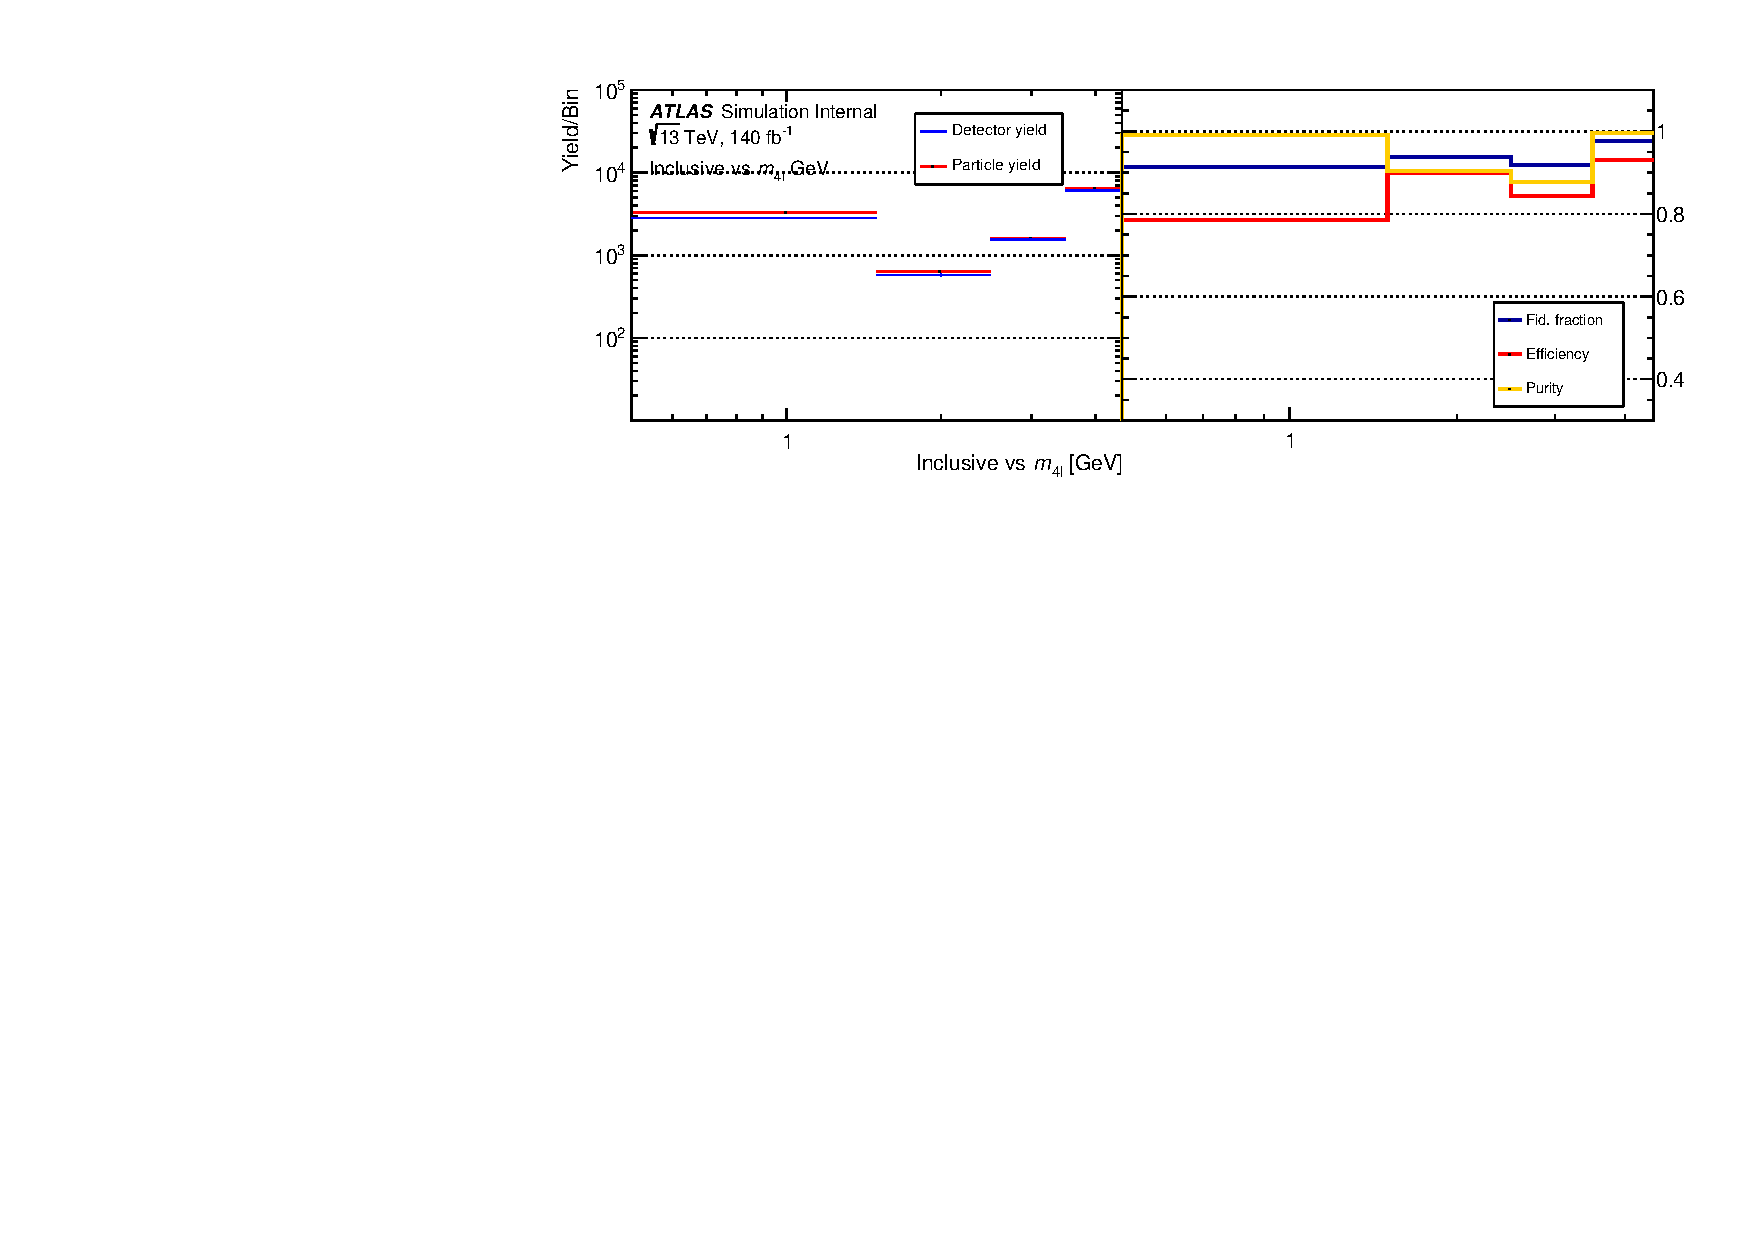
\includegraphics[width=.99\linewidth]{Figures/m4l/UnfoldingStudies/v014_inputs/inclusive_vs_m4linputs.pdf}  
%    \end{subfigure}
%    \caption{In the left-hand panel, the number of predicted events passing the reconstruction- and fiducial- level selections are displayed as the detector yield and particle yield, respectively. They are given as a function of the four \mFourL regions: single Z, Higgs,  offshell ZZ, and onshell ZZ in that order. The right-hand panel shows the efficiency, fiducial purity and fiducial fraction in each of the same \mFourL regions.}
%    \label{fig:inclvm4lunf}
%\end{figure}
%%double differentials
\begin{figure}[htb]
    \begin{subfigure}{.99\textwidth}\centering
        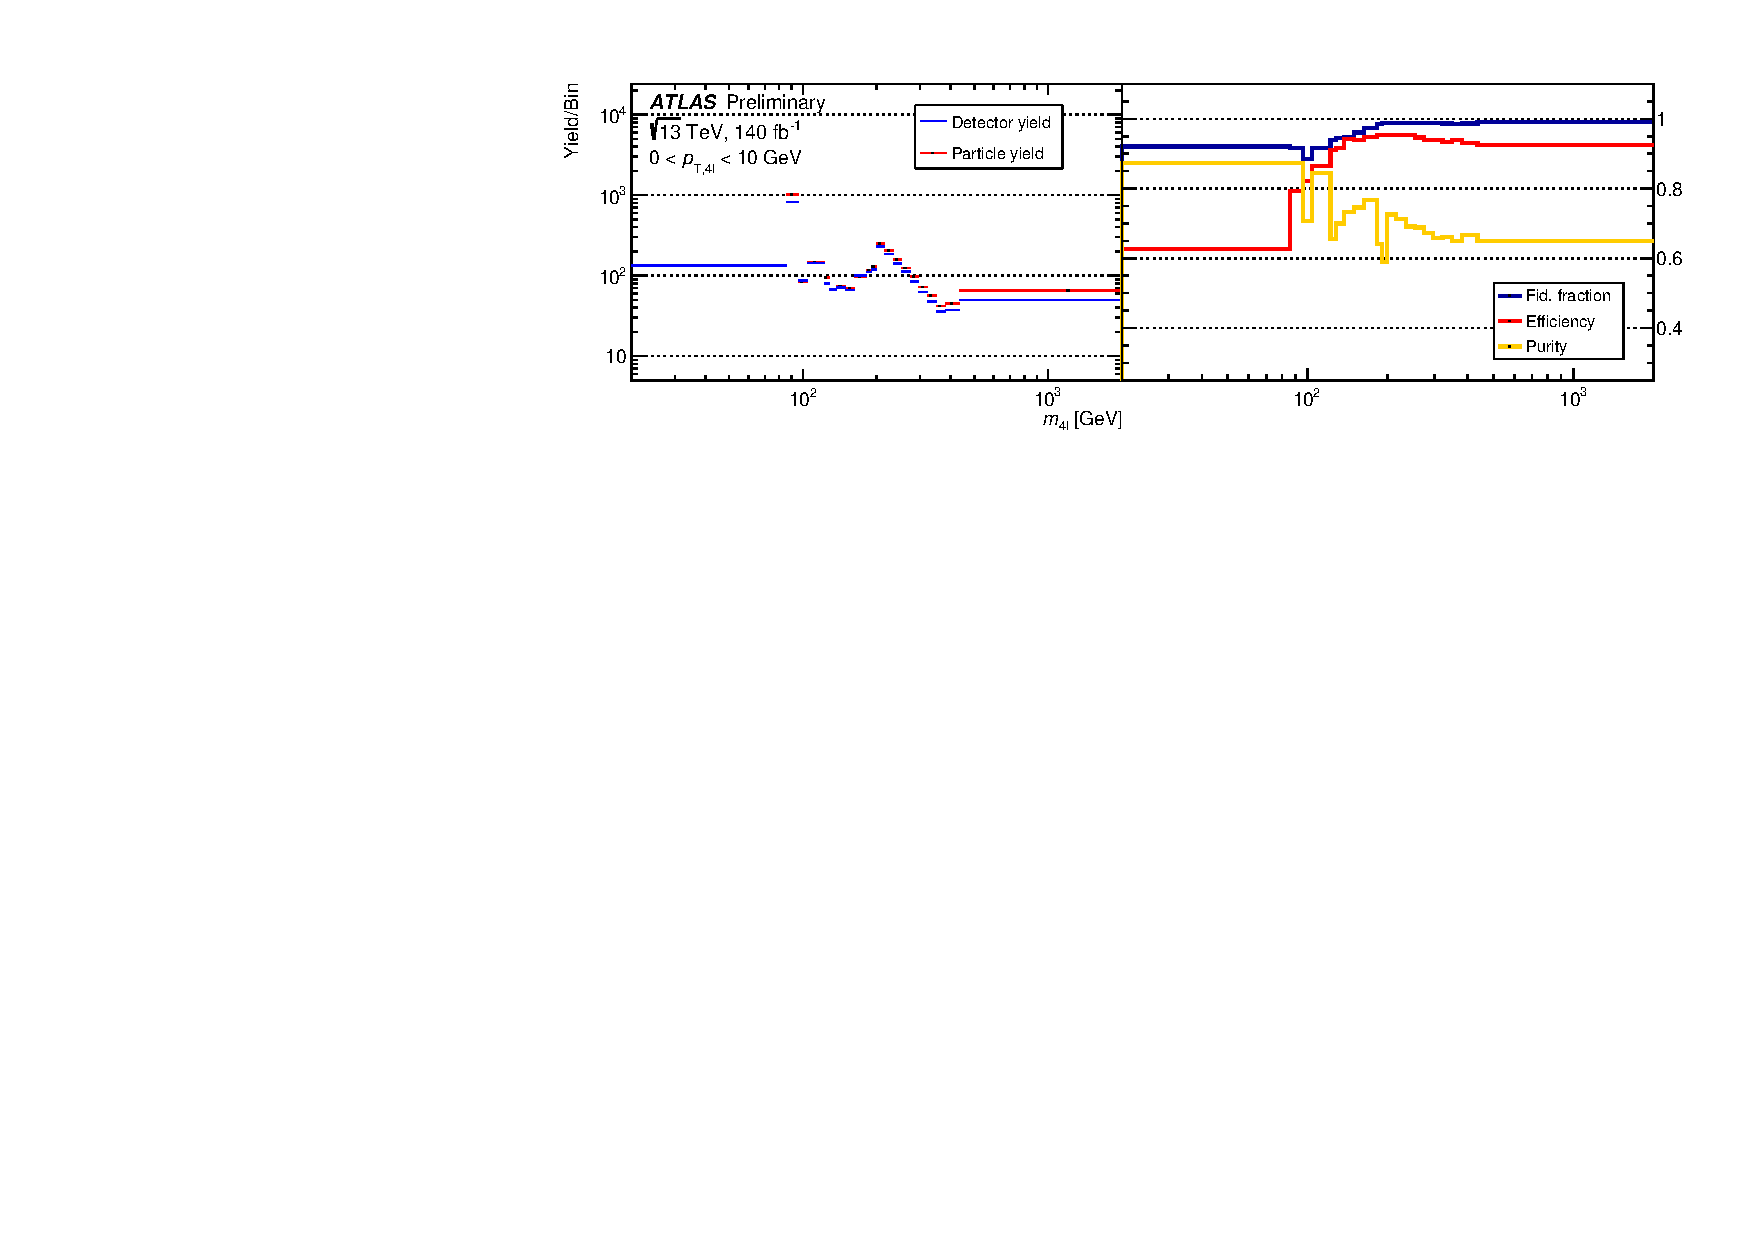
\includegraphics[width = 0.75\textwidth]{Figures/m4l/UnfoldingStudies/v014_inputs/m4l_pt4l0-10inputs.pdf}
    \end{subfigure}
    \begin{subfigure}{.99\textwidth}\centering
        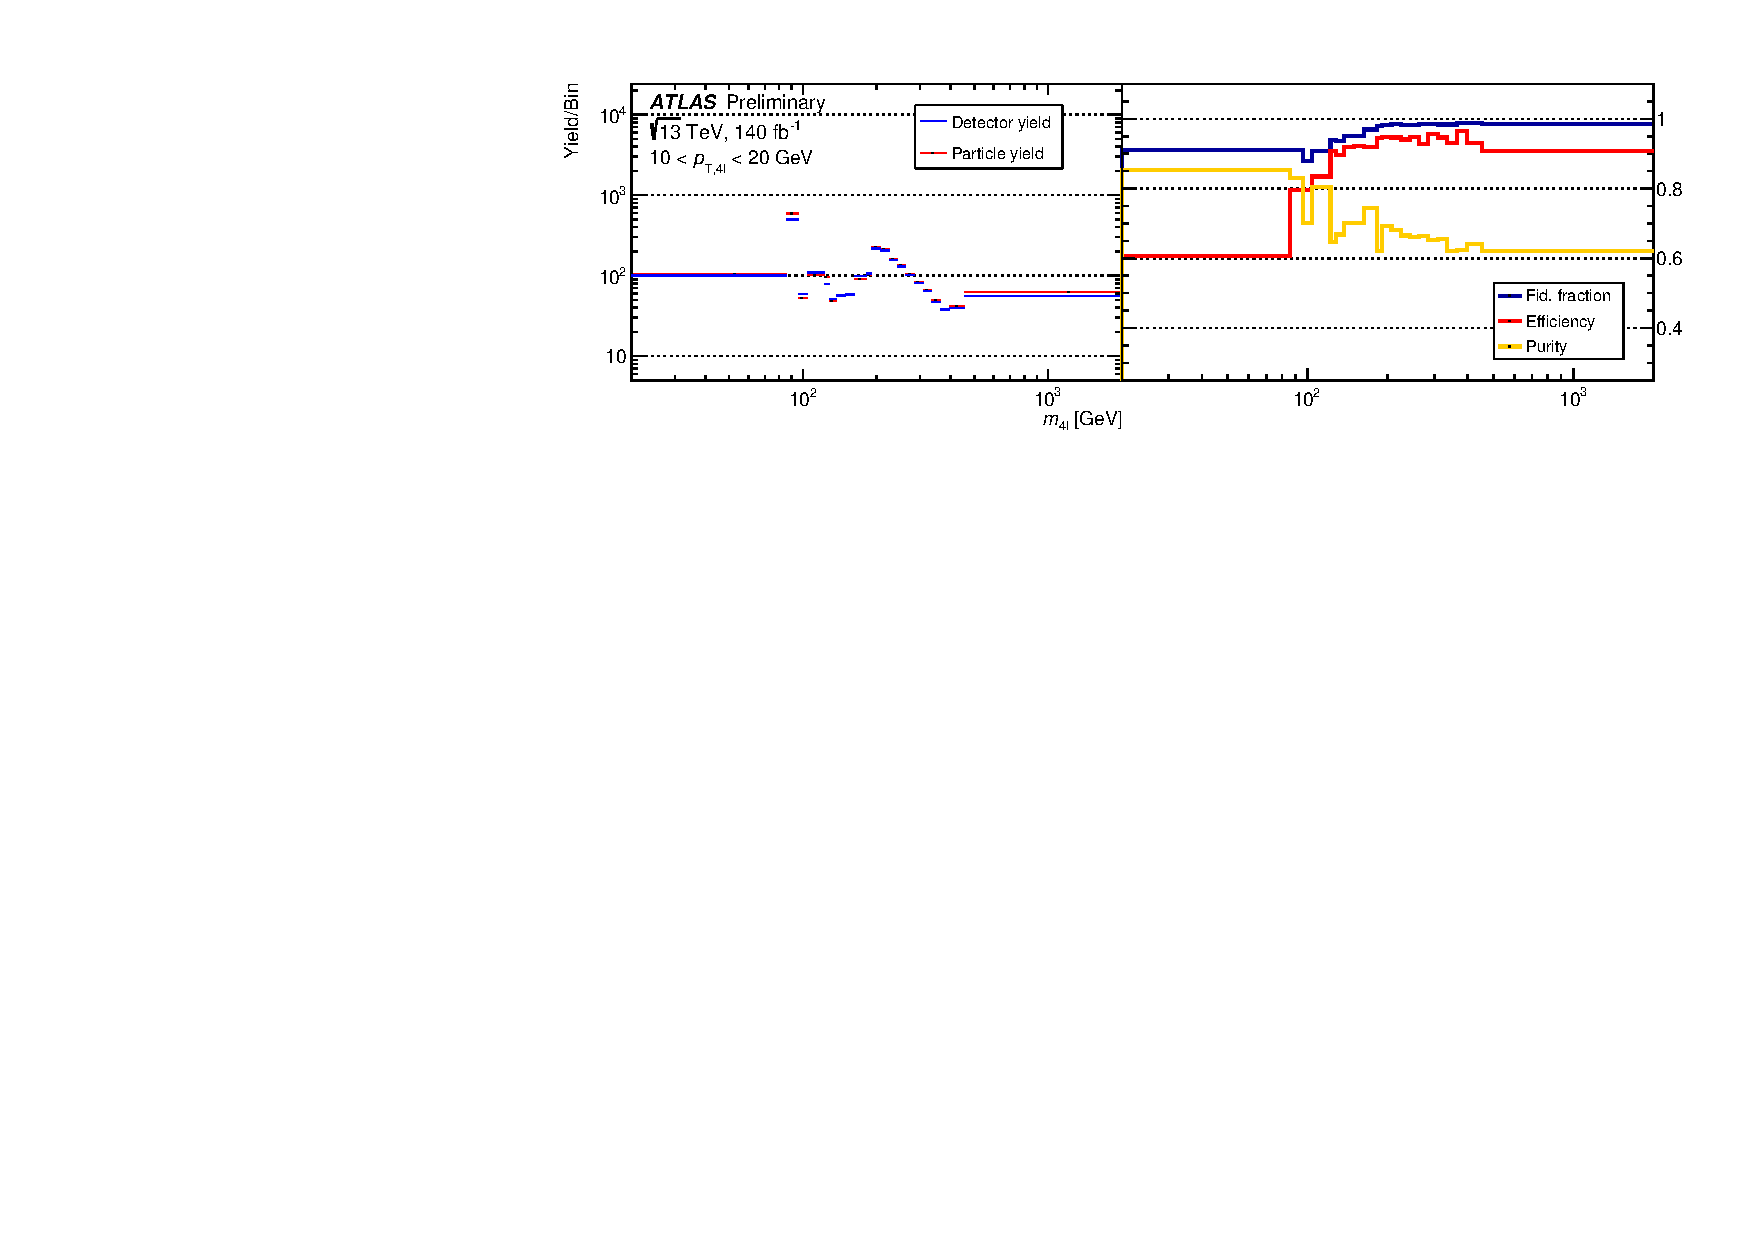
\includegraphics[width = 0.75\textwidth]{Figures/m4l/UnfoldingStudies/v014_inputs/m4l_pt4l10-20inputs.pdf}
    \end{subfigure}
    \begin{subfigure}{.99\textwidth}\centering
        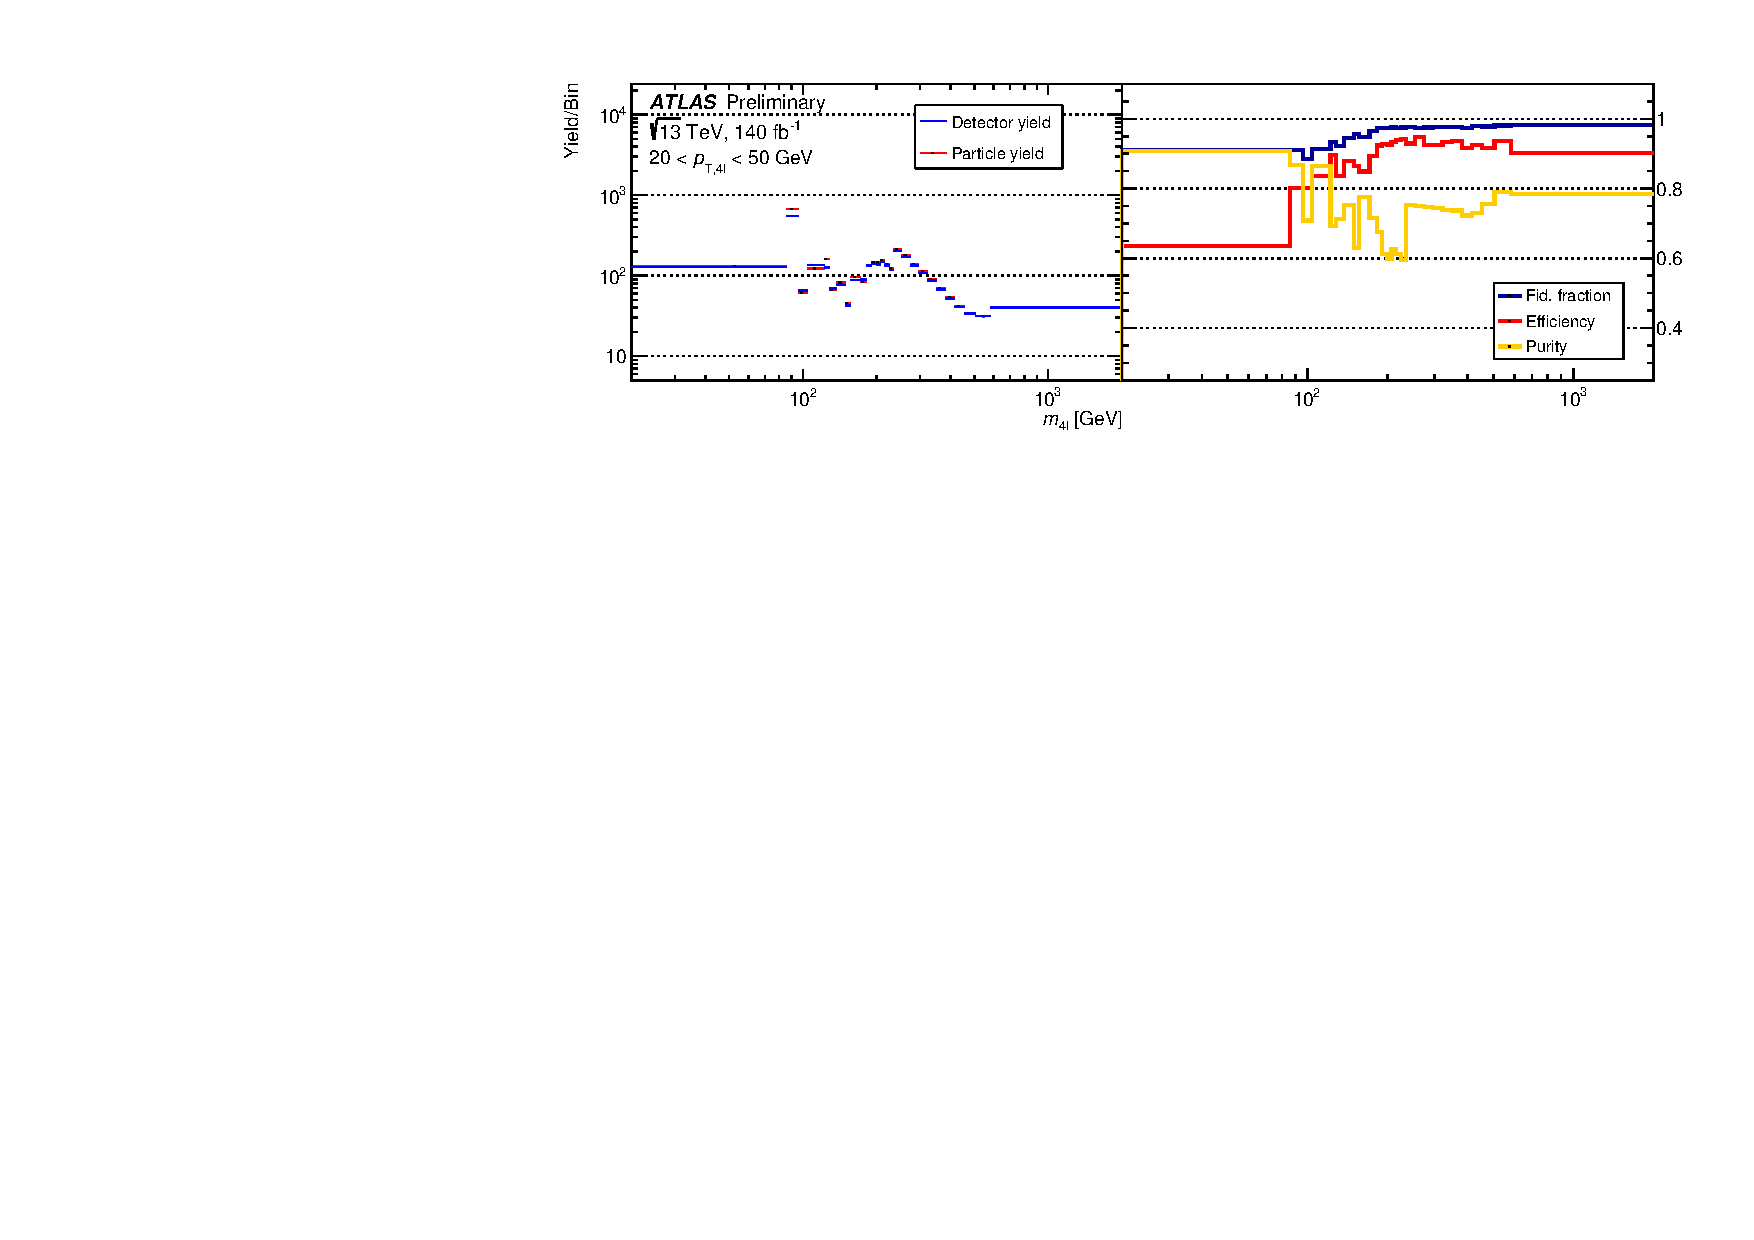
\includegraphics[width = 0.75\textwidth]{Figures/m4l/UnfoldingStudies/v014_inputs/m4l_pt4l20-50inputs.pdf}
    \end{subfigure}
    \begin{subfigure}{.99\textwidth}\centering
        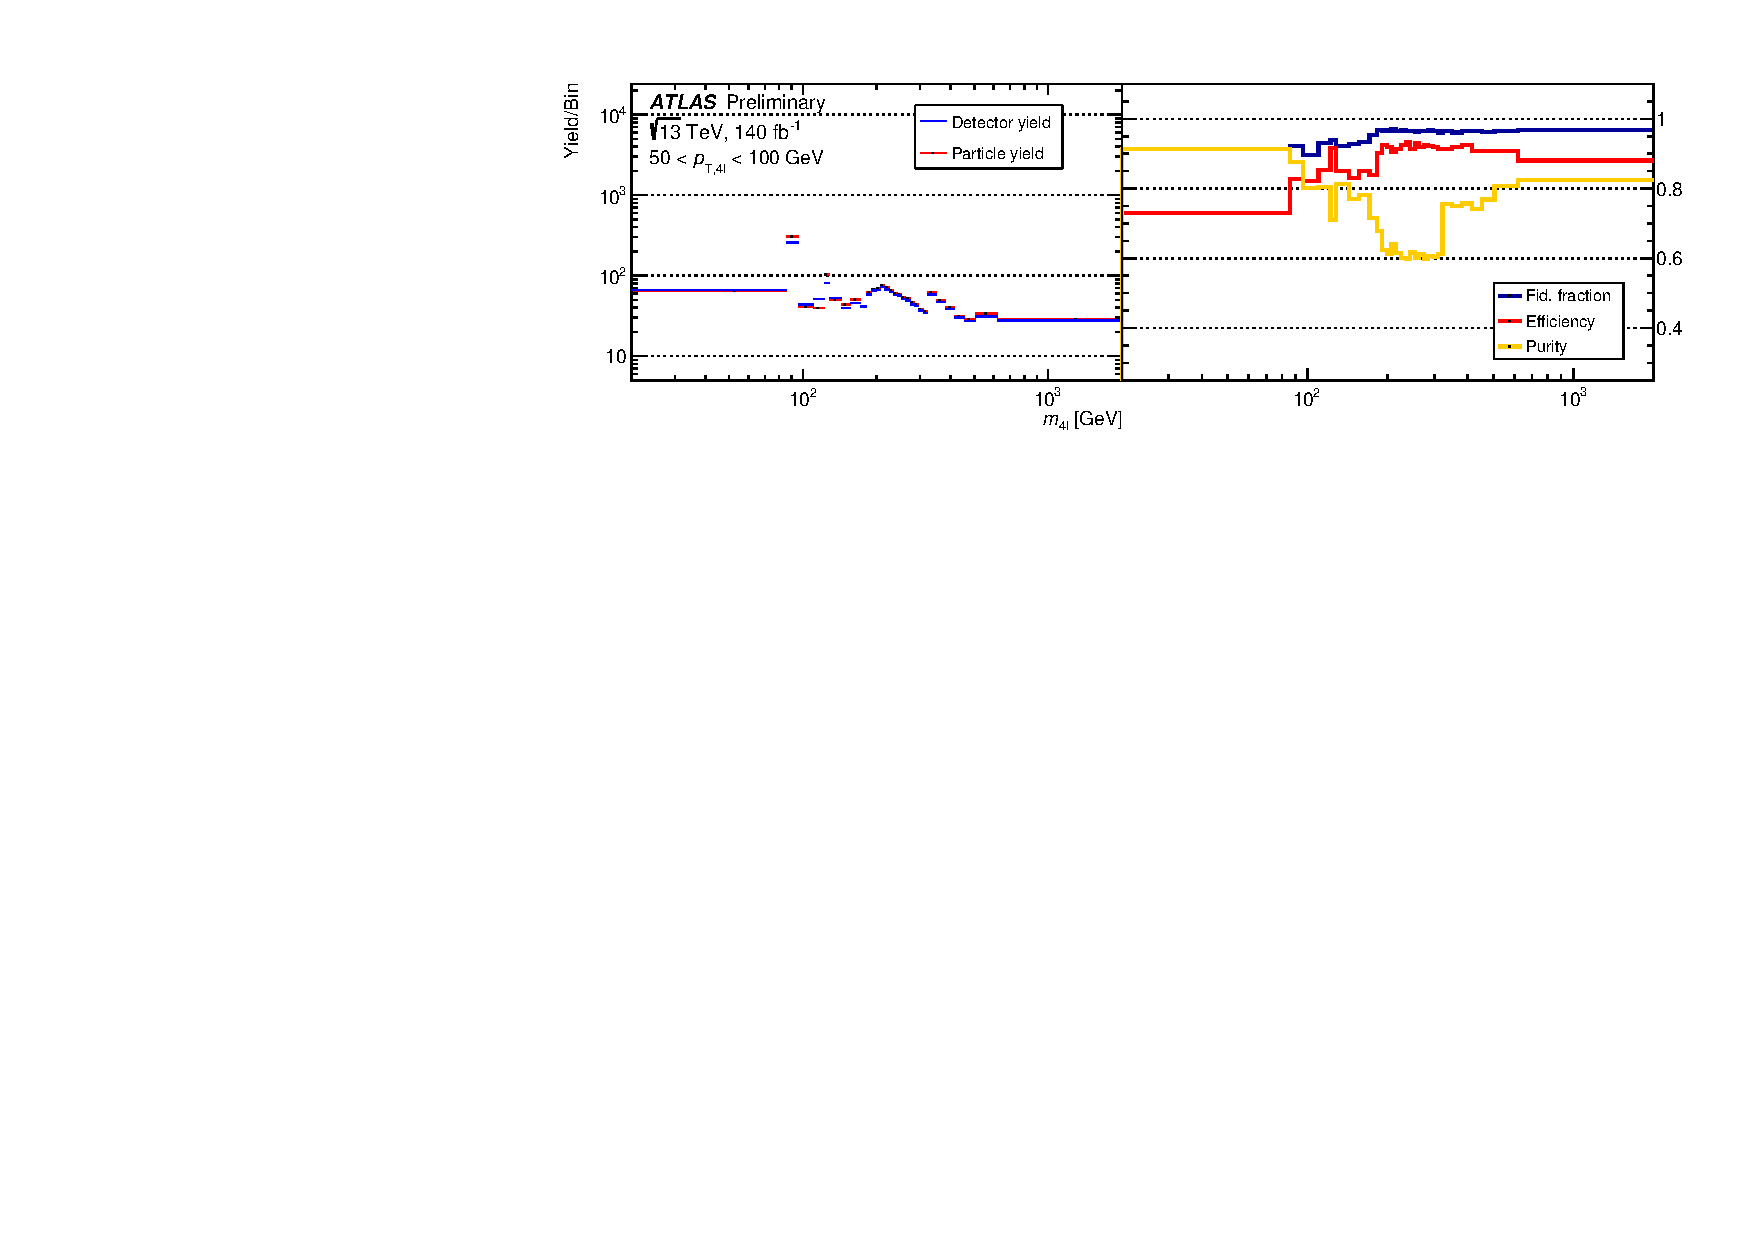
\includegraphics[width = 0.75\textwidth]{Figures/m4l/UnfoldingStudies/v014_inputs/m4l_pt4l50-100inputs.pdf}
    \end{subfigure}
    \begin{subfigure}{.99\textwidth}\centering
        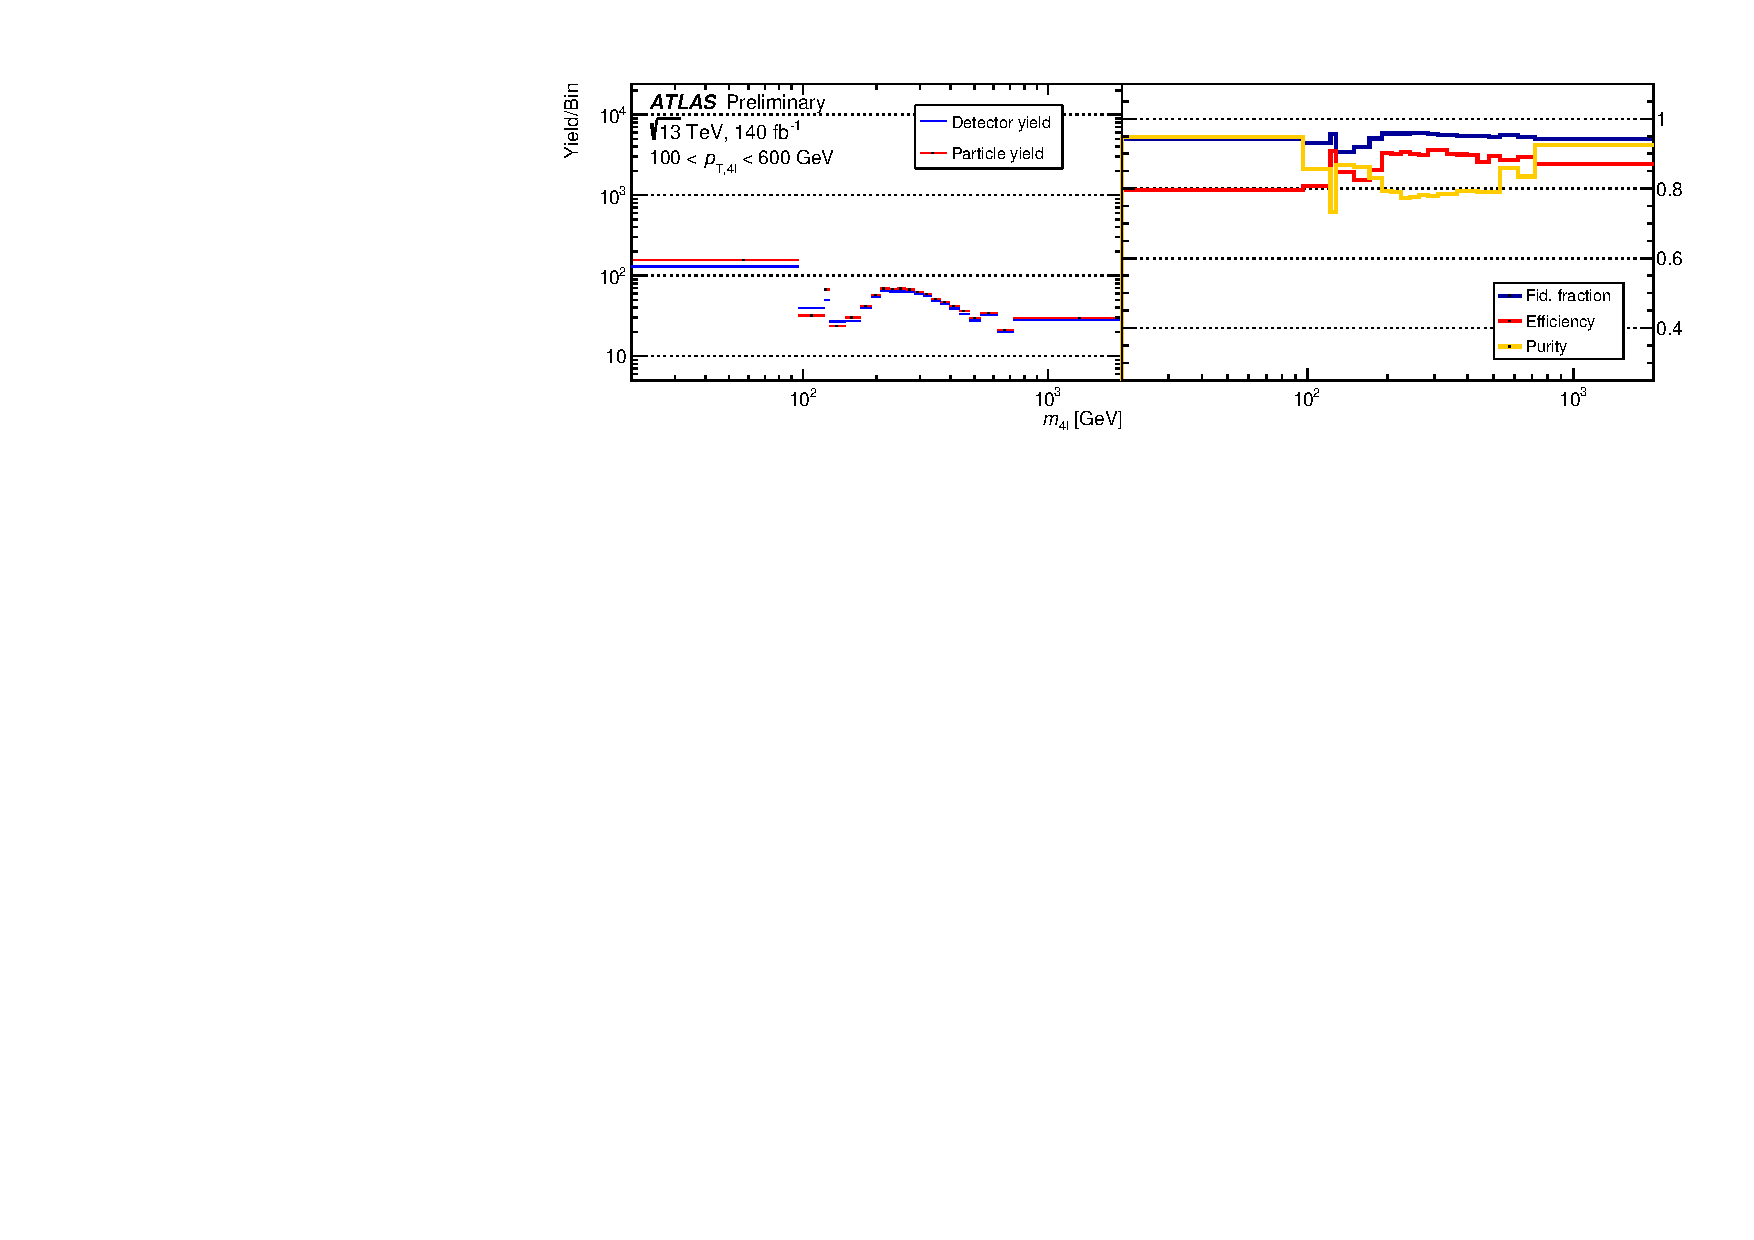
\includegraphics[width = 0.75\textwidth]{Figures/m4l/UnfoldingStudies/v014_inputs/m4l_pt4l100-600inputs.pdf}
    \end{subfigure}   
    \caption{In the left-hand panels, the number of predicted events passing the reconstruction- and fiducial- level selections are displayed as the detector yield and particle yield, respectively. The right-hand panel shows the efficiency, fiducial purity and fiducial fraction. All variables are plotted as a function of the \mFourL bins, in slices of the \ptFourL variable which are stacked and labelled with the included \ptFourL range.
    \label{fig:pt4lunf}}
\end{figure}  

\FloatBarrier
\clearpage

%y4l
\begin{figure}[htb]
    \centering 
    \begin{subfigure}{.99\textwidth}\centering
      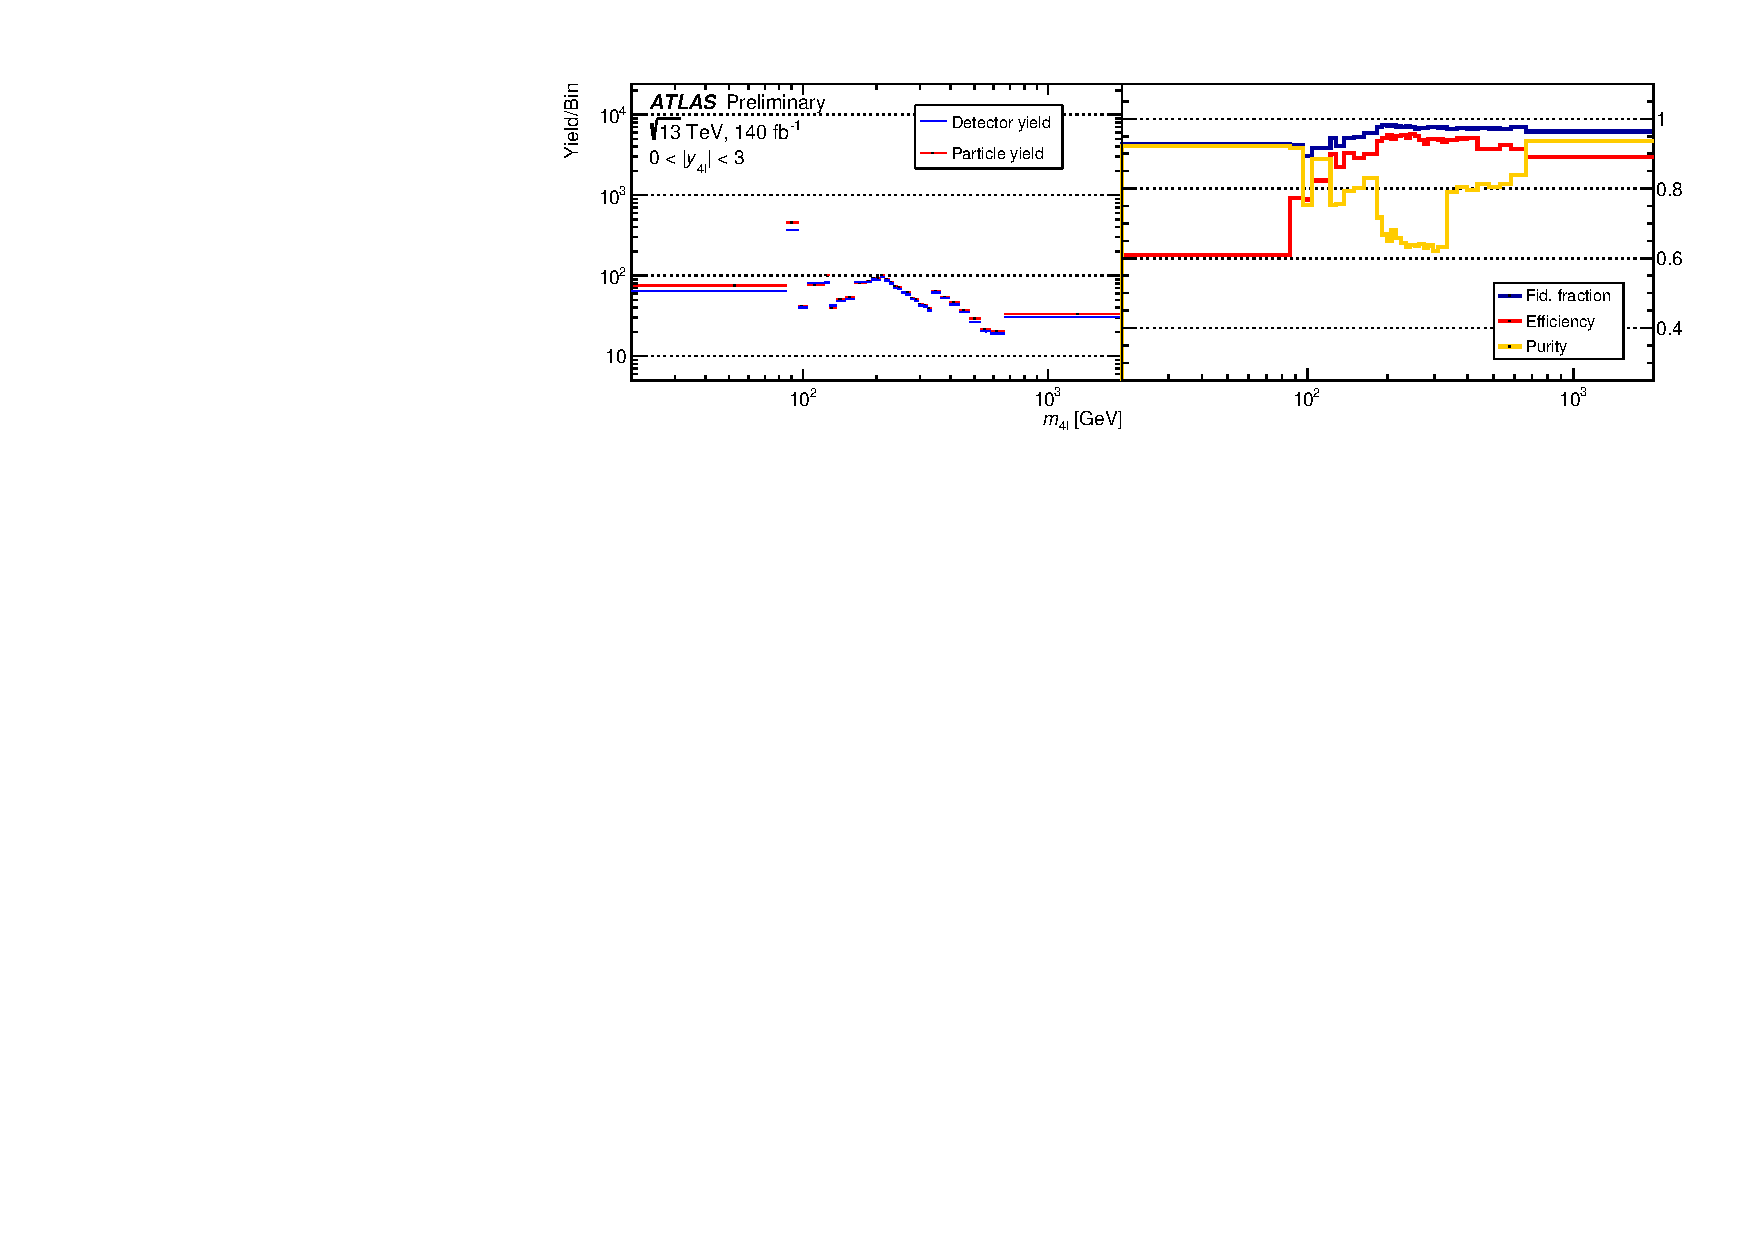
\includegraphics[width = 0.75\textwidth]{Figures/m4l/UnfoldingStudies/v014_inputs/m4l_y4l0-3inputs.pdf}
    \end{subfigure}
    \begin{subfigure}{.99\textwidth}\centering
      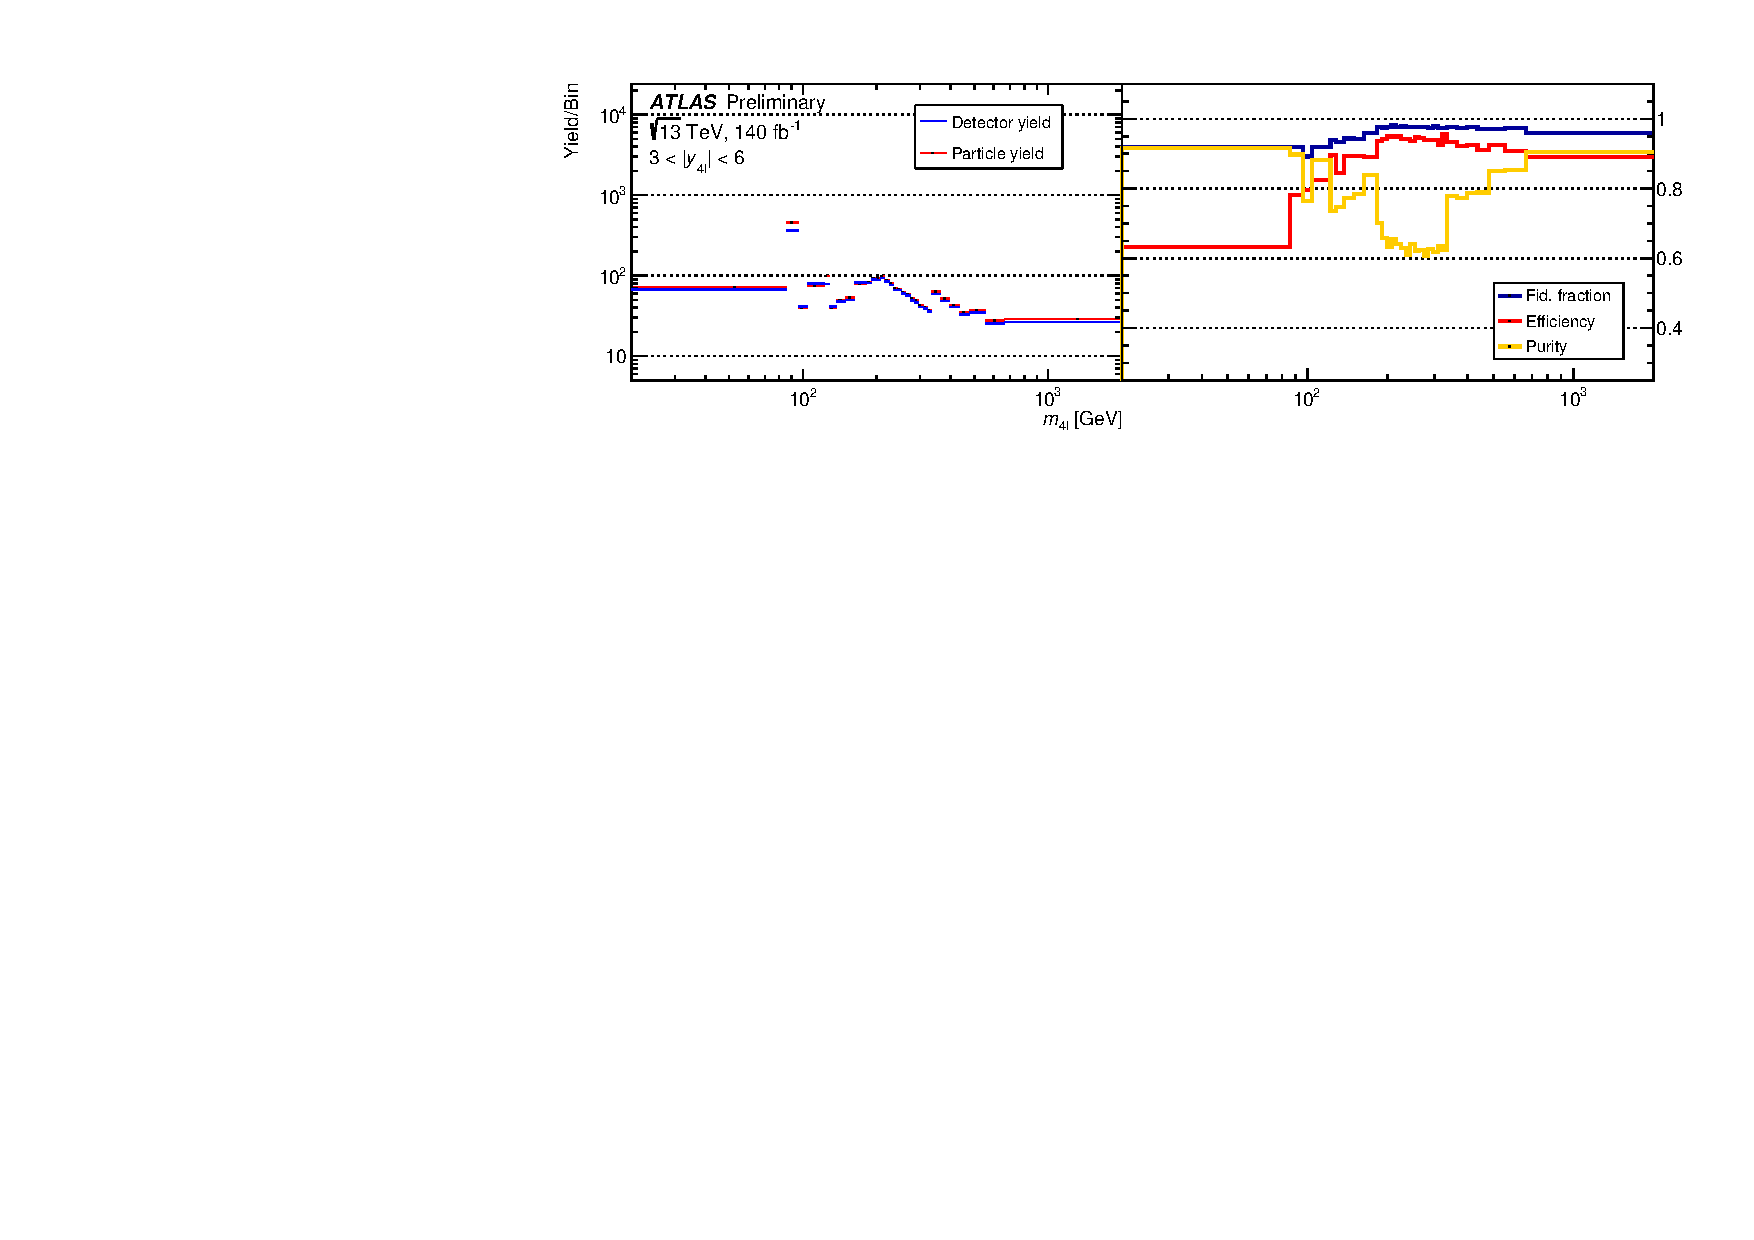
\includegraphics[width = 0.75\textwidth]{Figures/m4l/UnfoldingStudies/v014_inputs/m4l_y4l3-6inputs.pdf}
    \end{subfigure}
    \begin{subfigure}{.99\textwidth}\centering
      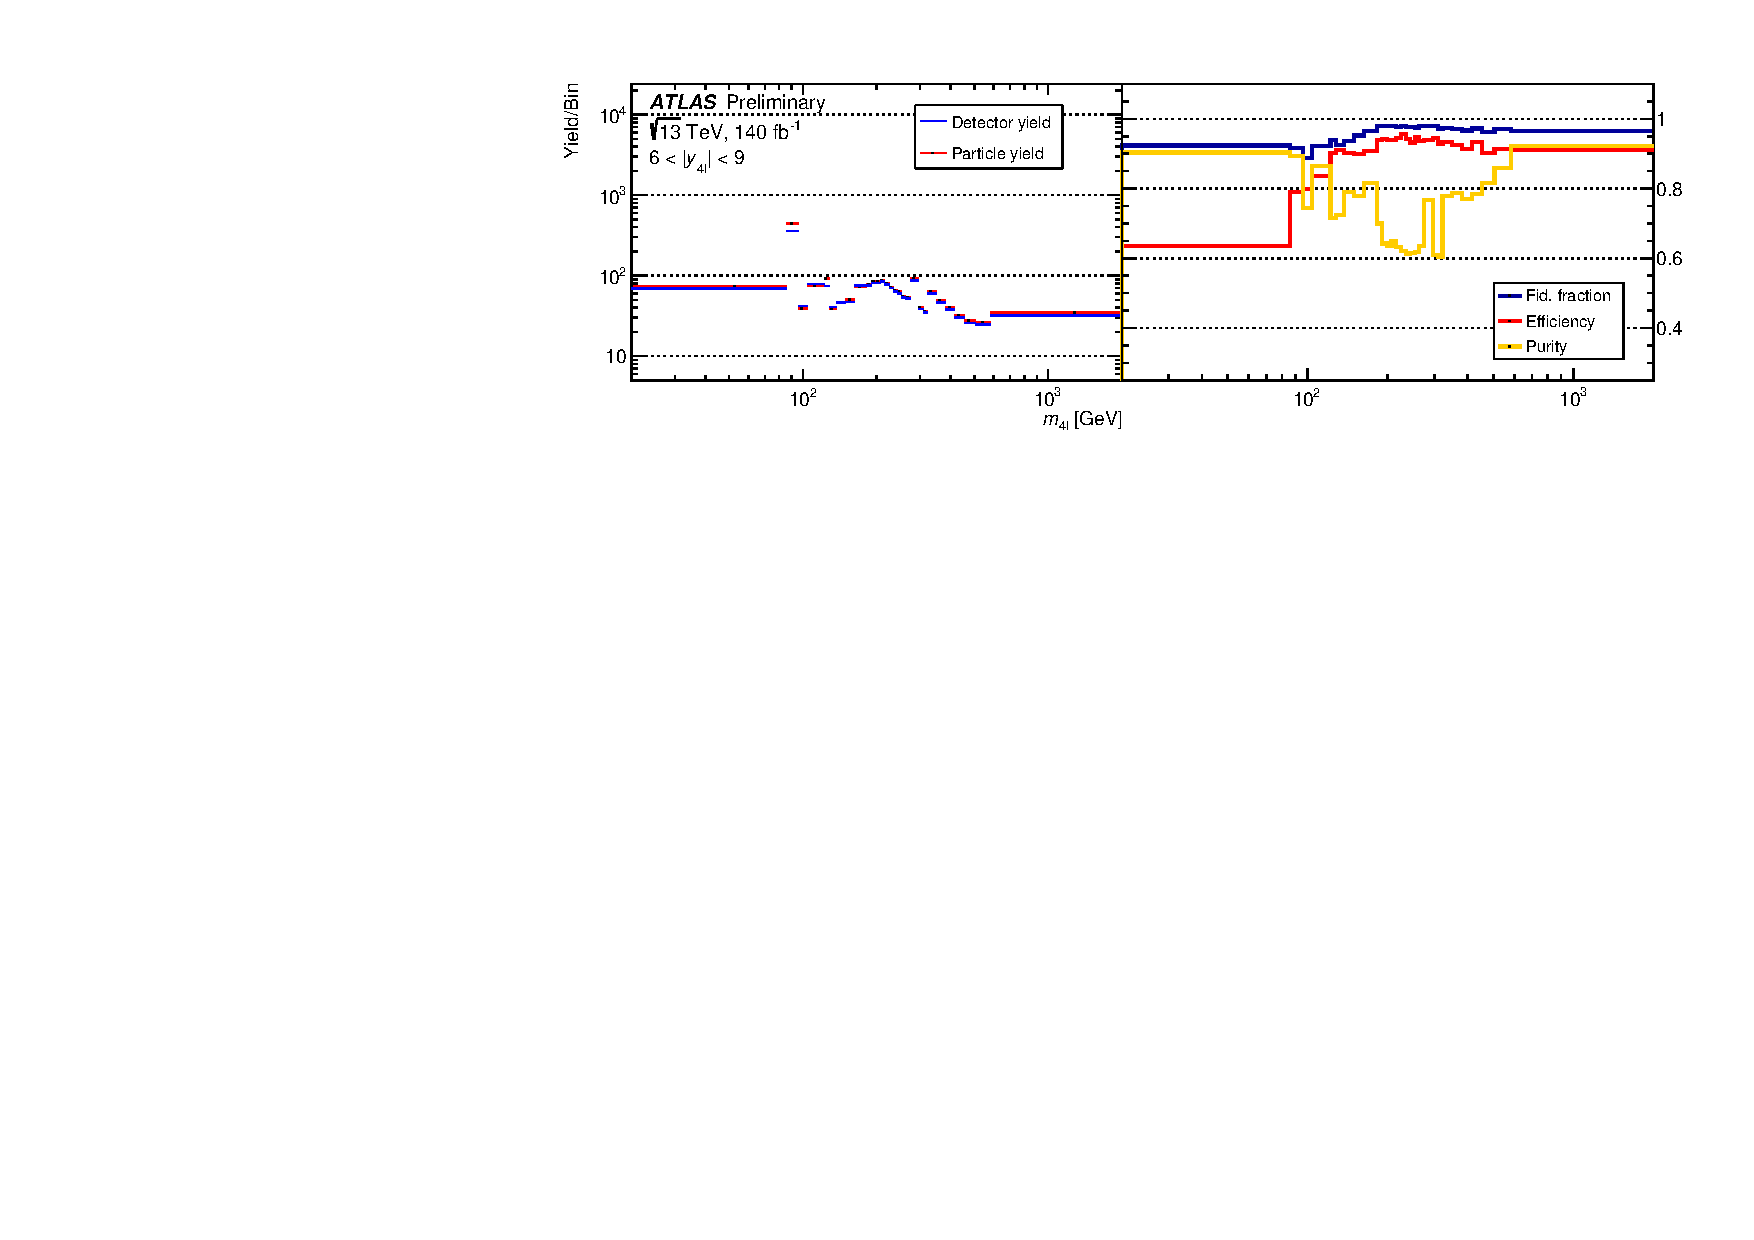
\includegraphics[width = 0.75\textwidth]{Figures/m4l/UnfoldingStudies/v014_inputs/m4l_y4l6-9inputs.pdf}
    \end{subfigure}
    \begin{subfigure}{.99\textwidth}\centering
      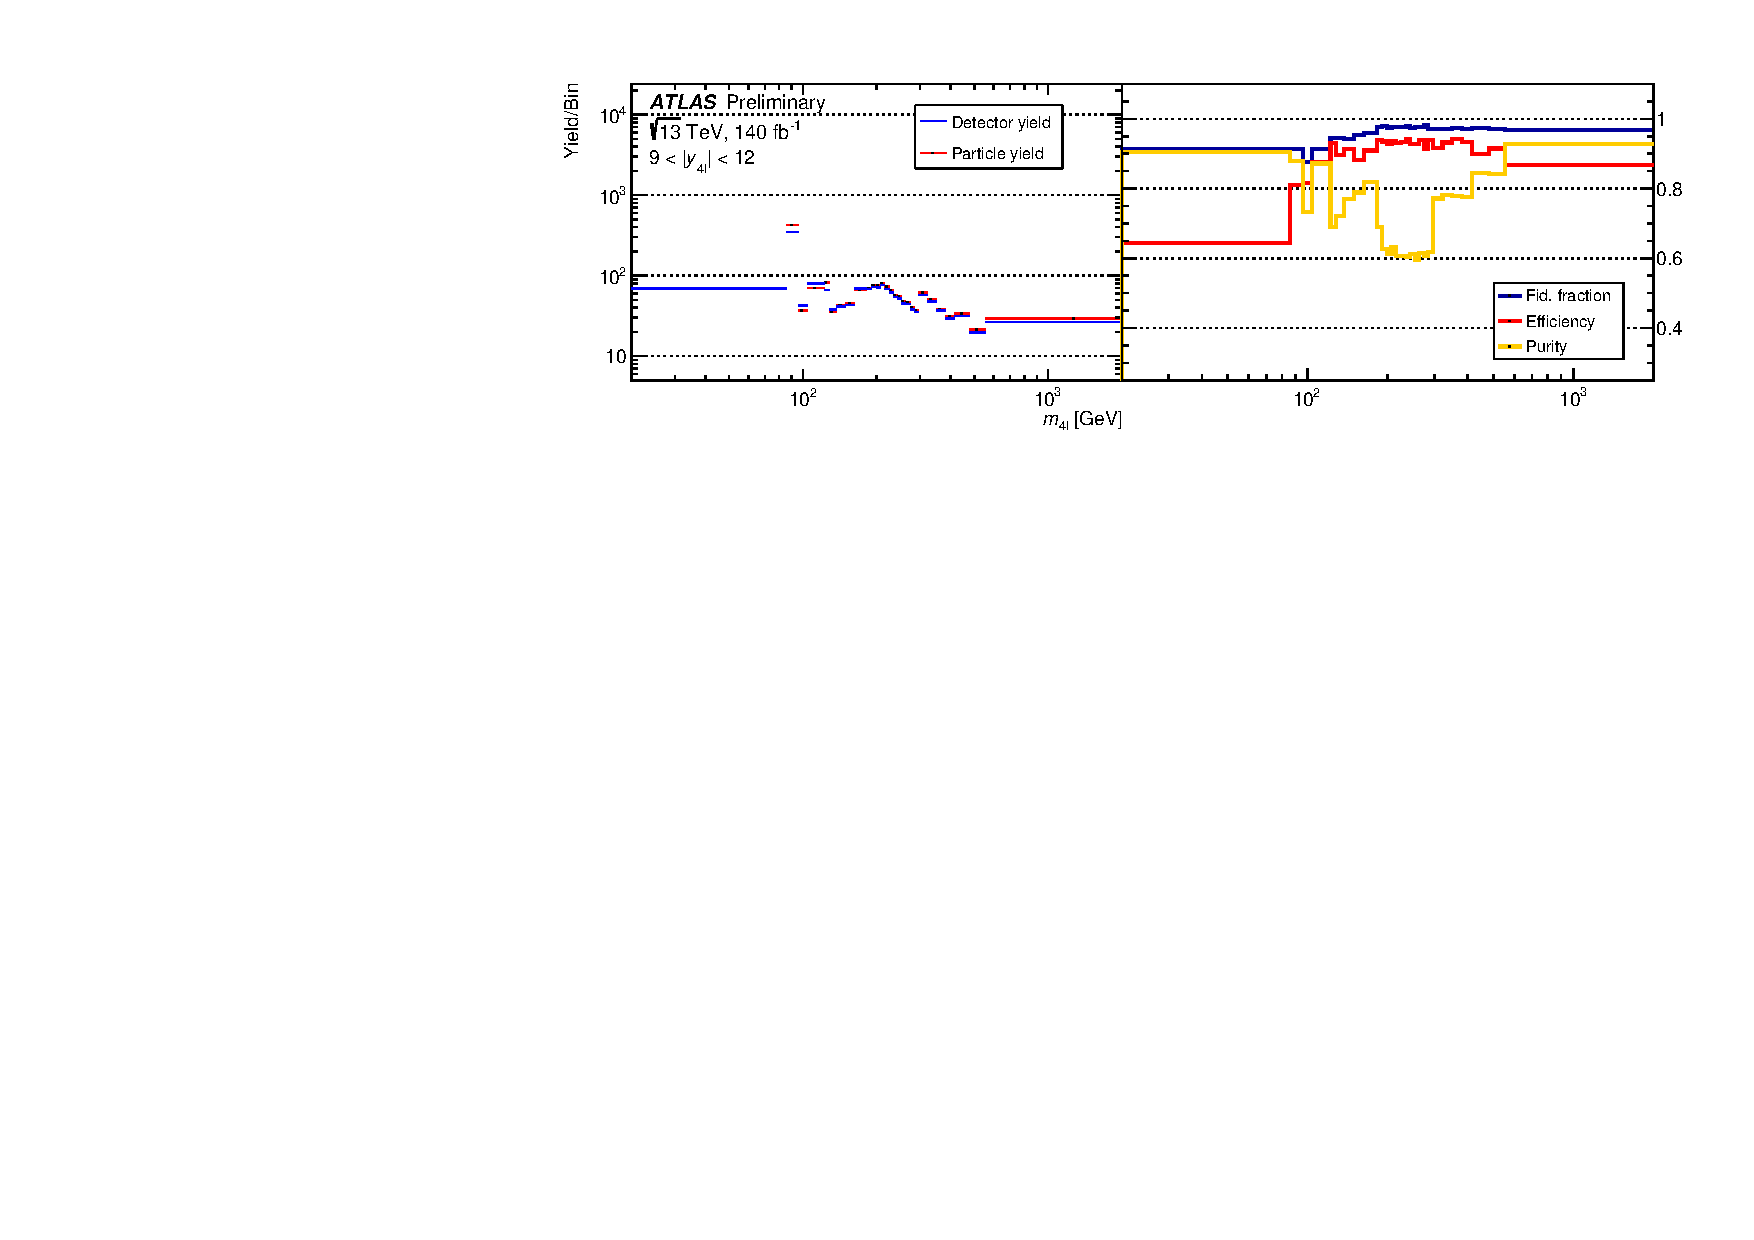
\includegraphics[width = 0.75\textwidth]{Figures/m4l/UnfoldingStudies/v014_inputs/m4l_y4l9-12inputs.pdf}
    \end{subfigure}
    \begin{subfigure}{.99\textwidth}\centering
      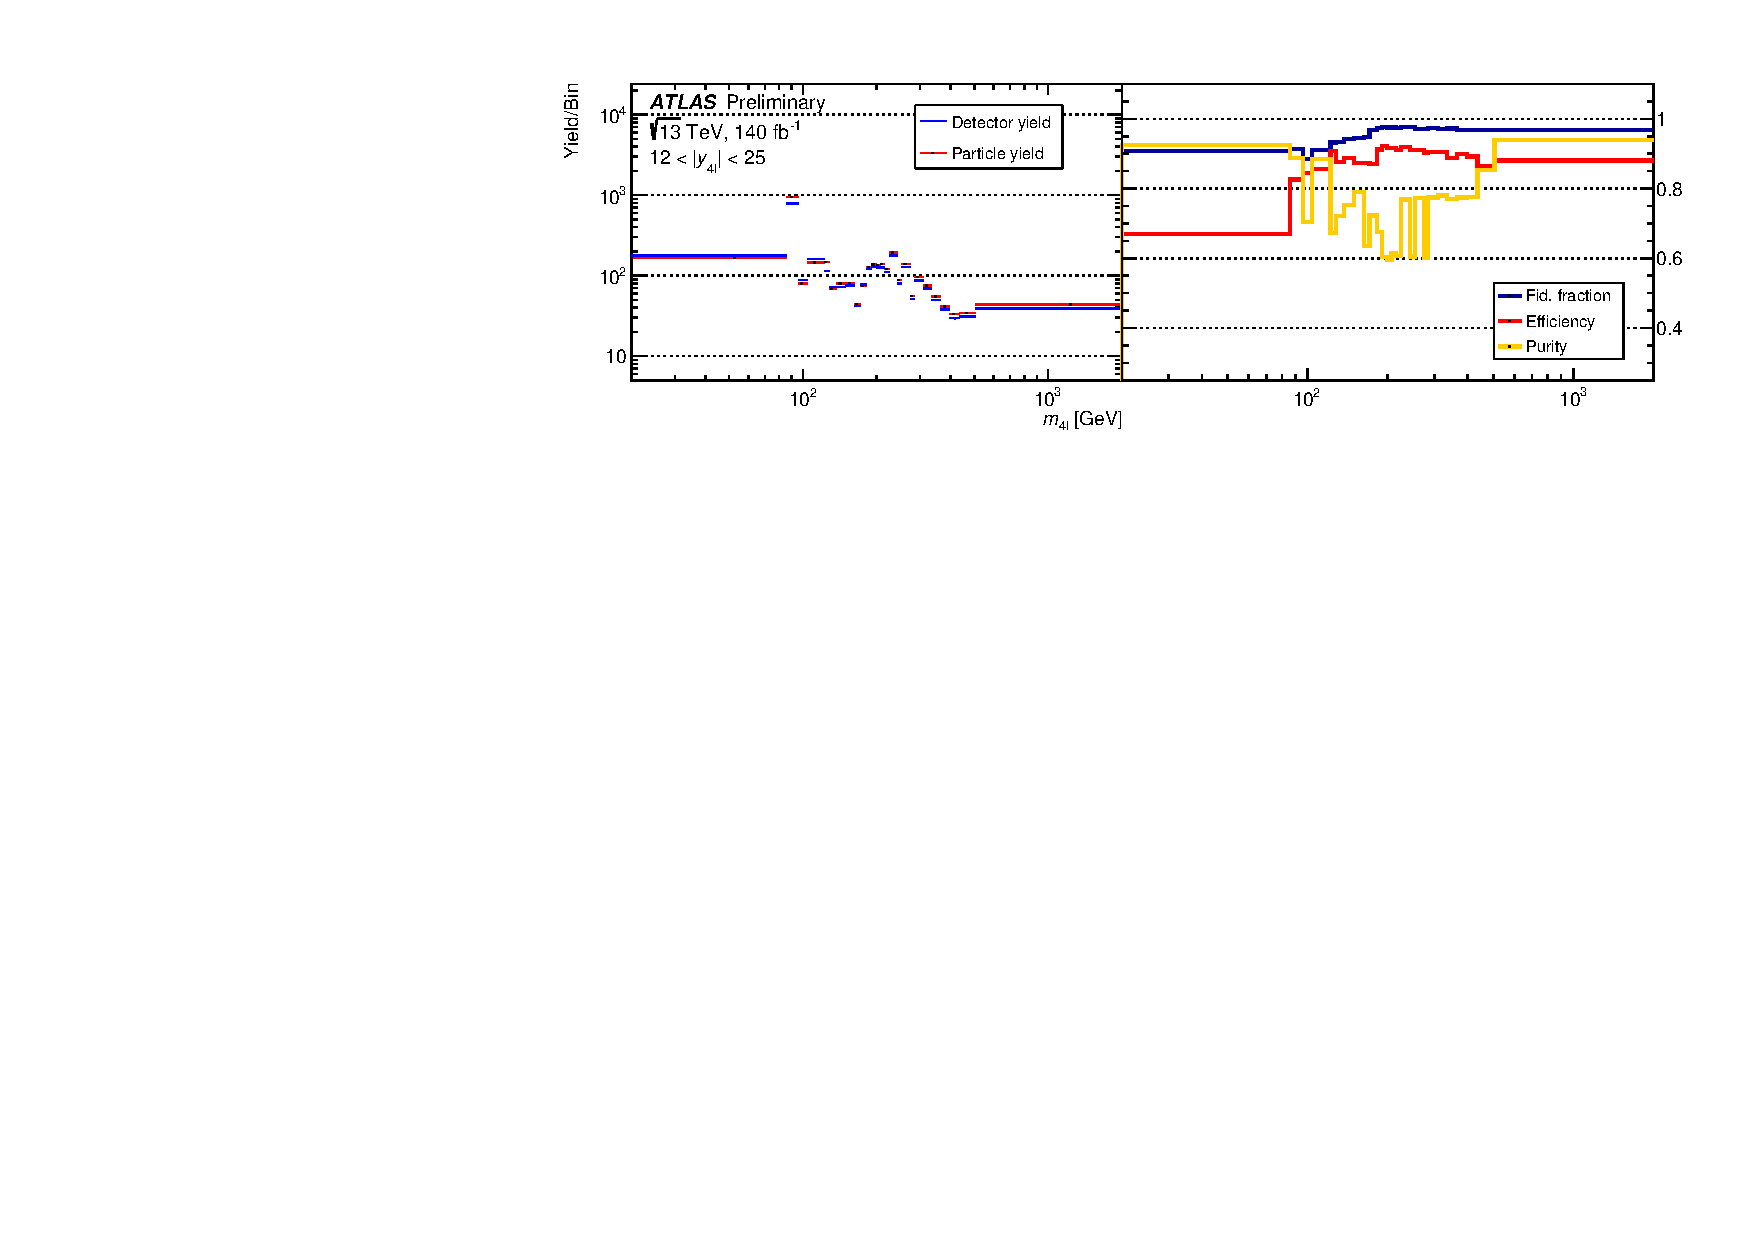
\includegraphics[width = 0.75\textwidth]{Figures/m4l/UnfoldingStudies/v014_inputs/m4l_y4l12-25inputs.pdf}
    \end{subfigure}
    \caption{In the left-hand panels, the number of predicted events passing the reconstruction- and fiducial- level selections are displayed as the detector yield and particle yield, respectively. The right-hand panel shows the efficiency, fiducial purity and fiducial fraction. All variables are plotted as a function of the \mFourL bins, in slices of the \yFourL variable which are stacked and labelled with the included \yFourL range.
    \label{fig:y4lunf}}
\end{figure}  

\FloatBarrier
\clearpage

\begin{figure}[htb]
    \centering 
    %elecs
    \begin{subfigure}{.99\textwidth}\centering
        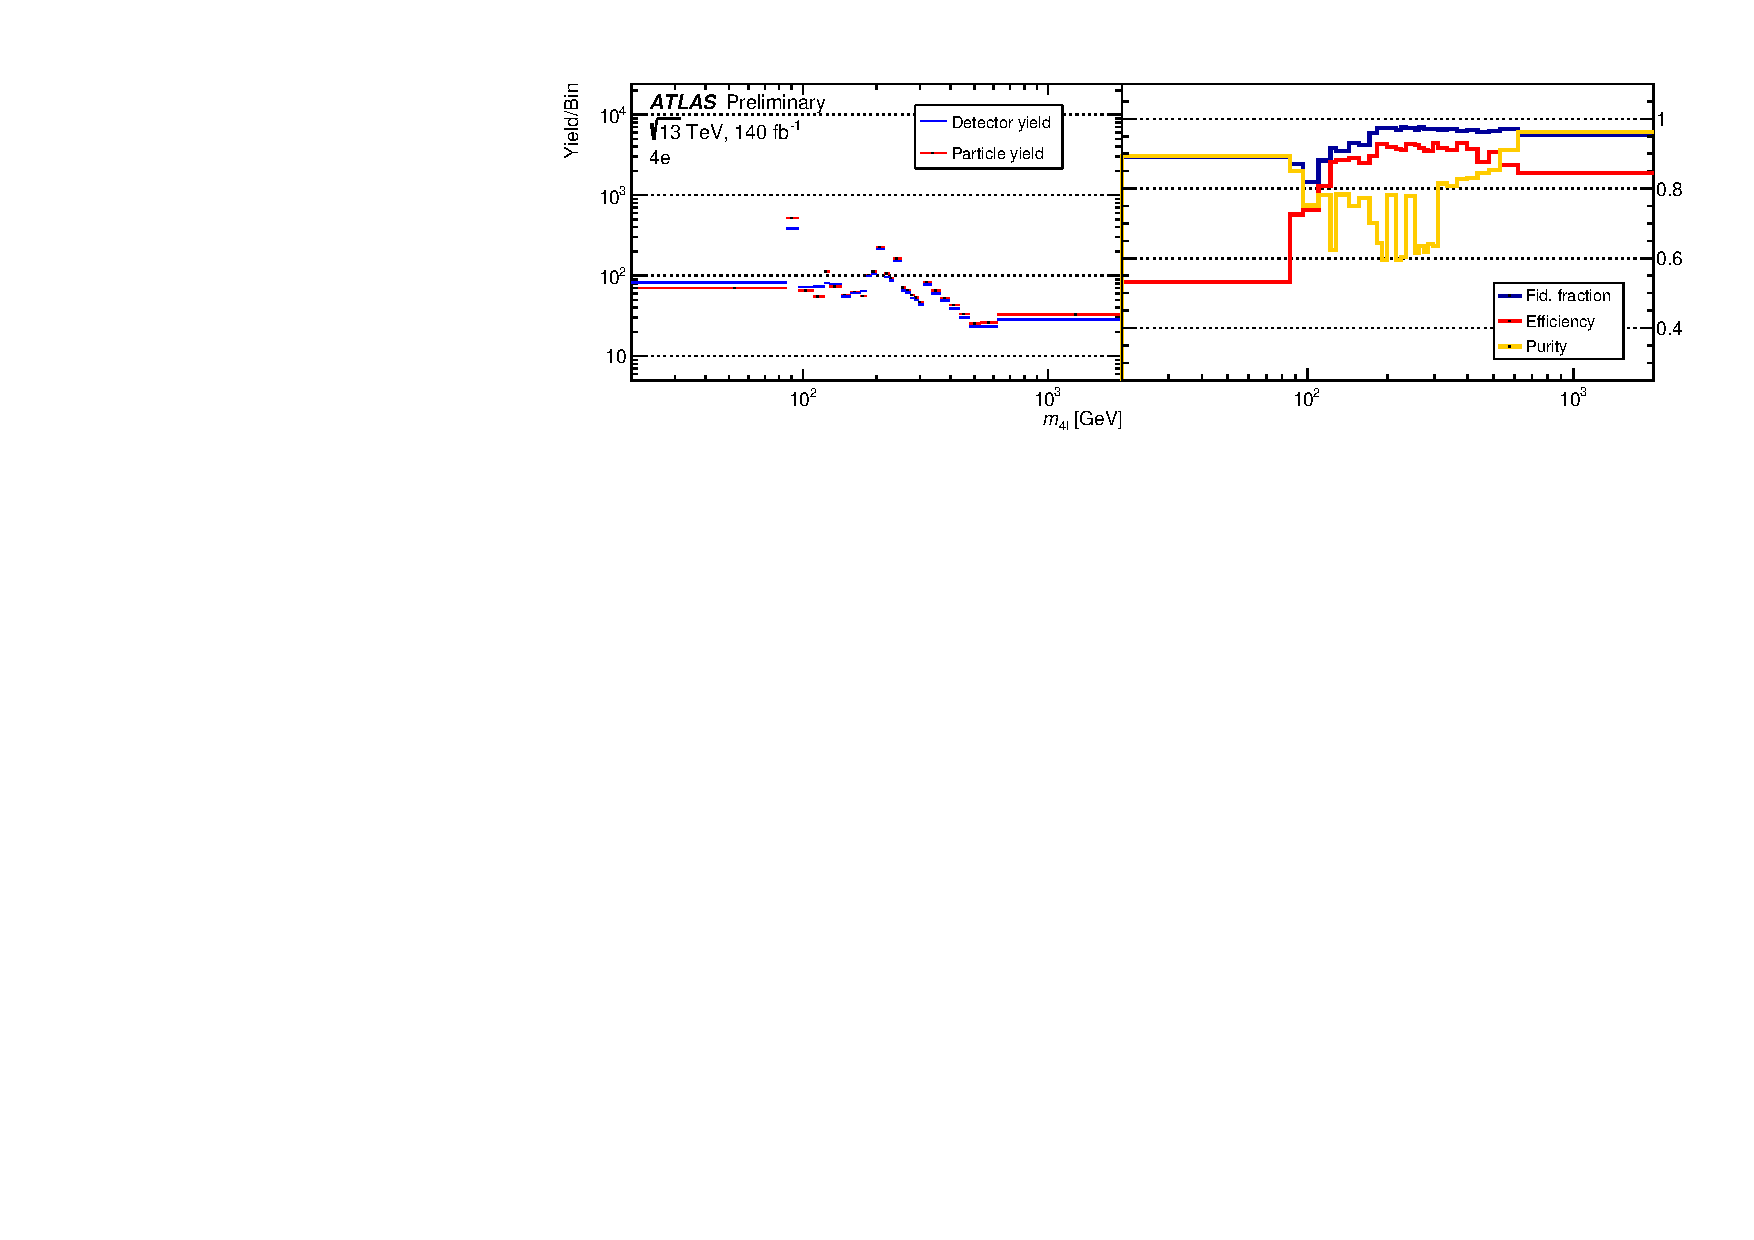
\includegraphics[width = 0.75\textwidth]{Figures/m4l/UnfoldingStudies/v014_inputs/m4l_event_type0-1inputs.pdf}
    \end{subfigure}
    %muons
    \begin{subfigure}{.99\textwidth}\centering
        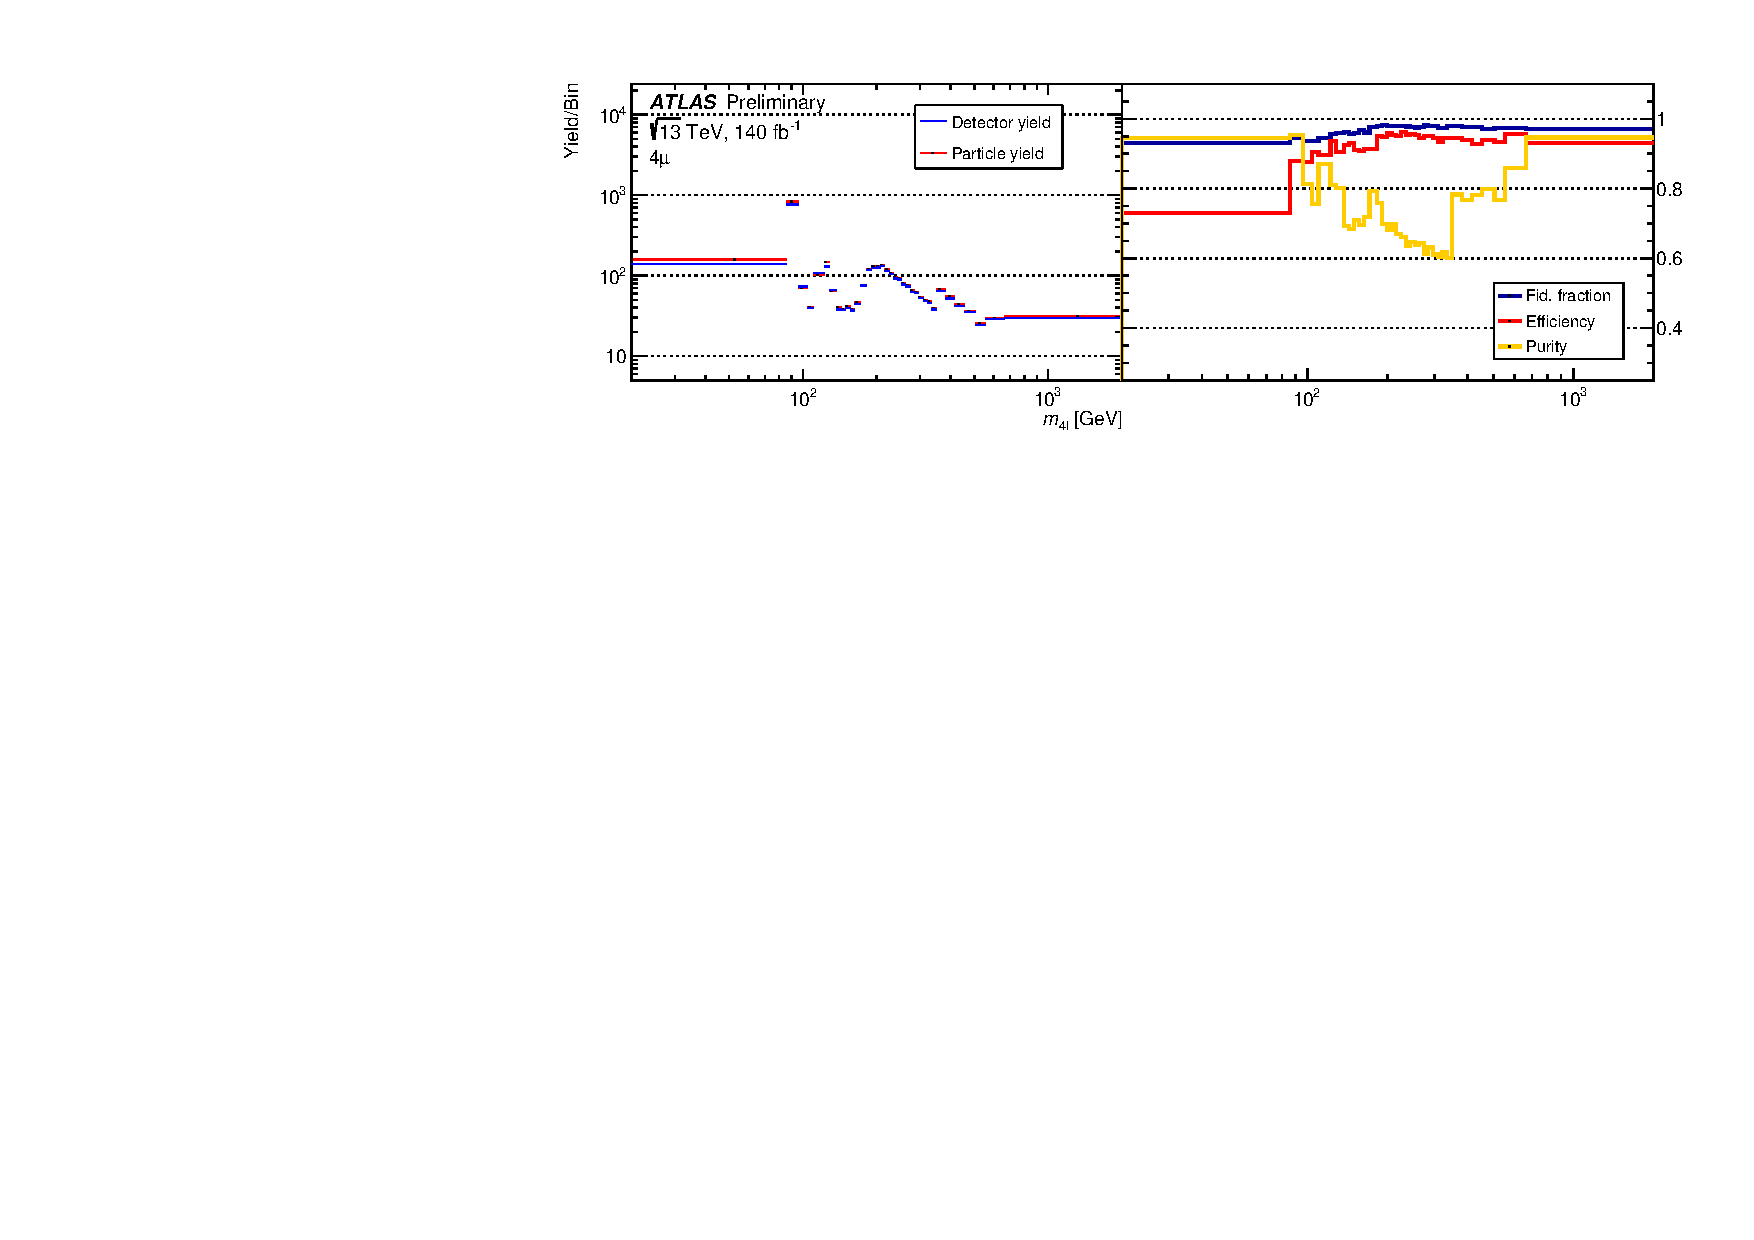
\includegraphics[width = 0.75\textwidth]{Figures/m4l/UnfoldingStudies/v014_inputs/m4l_event_type0-0inputs.pdf}
    \end{subfigure}
    %2mu2e
    \begin{subfigure}{.99\textwidth}\centering
        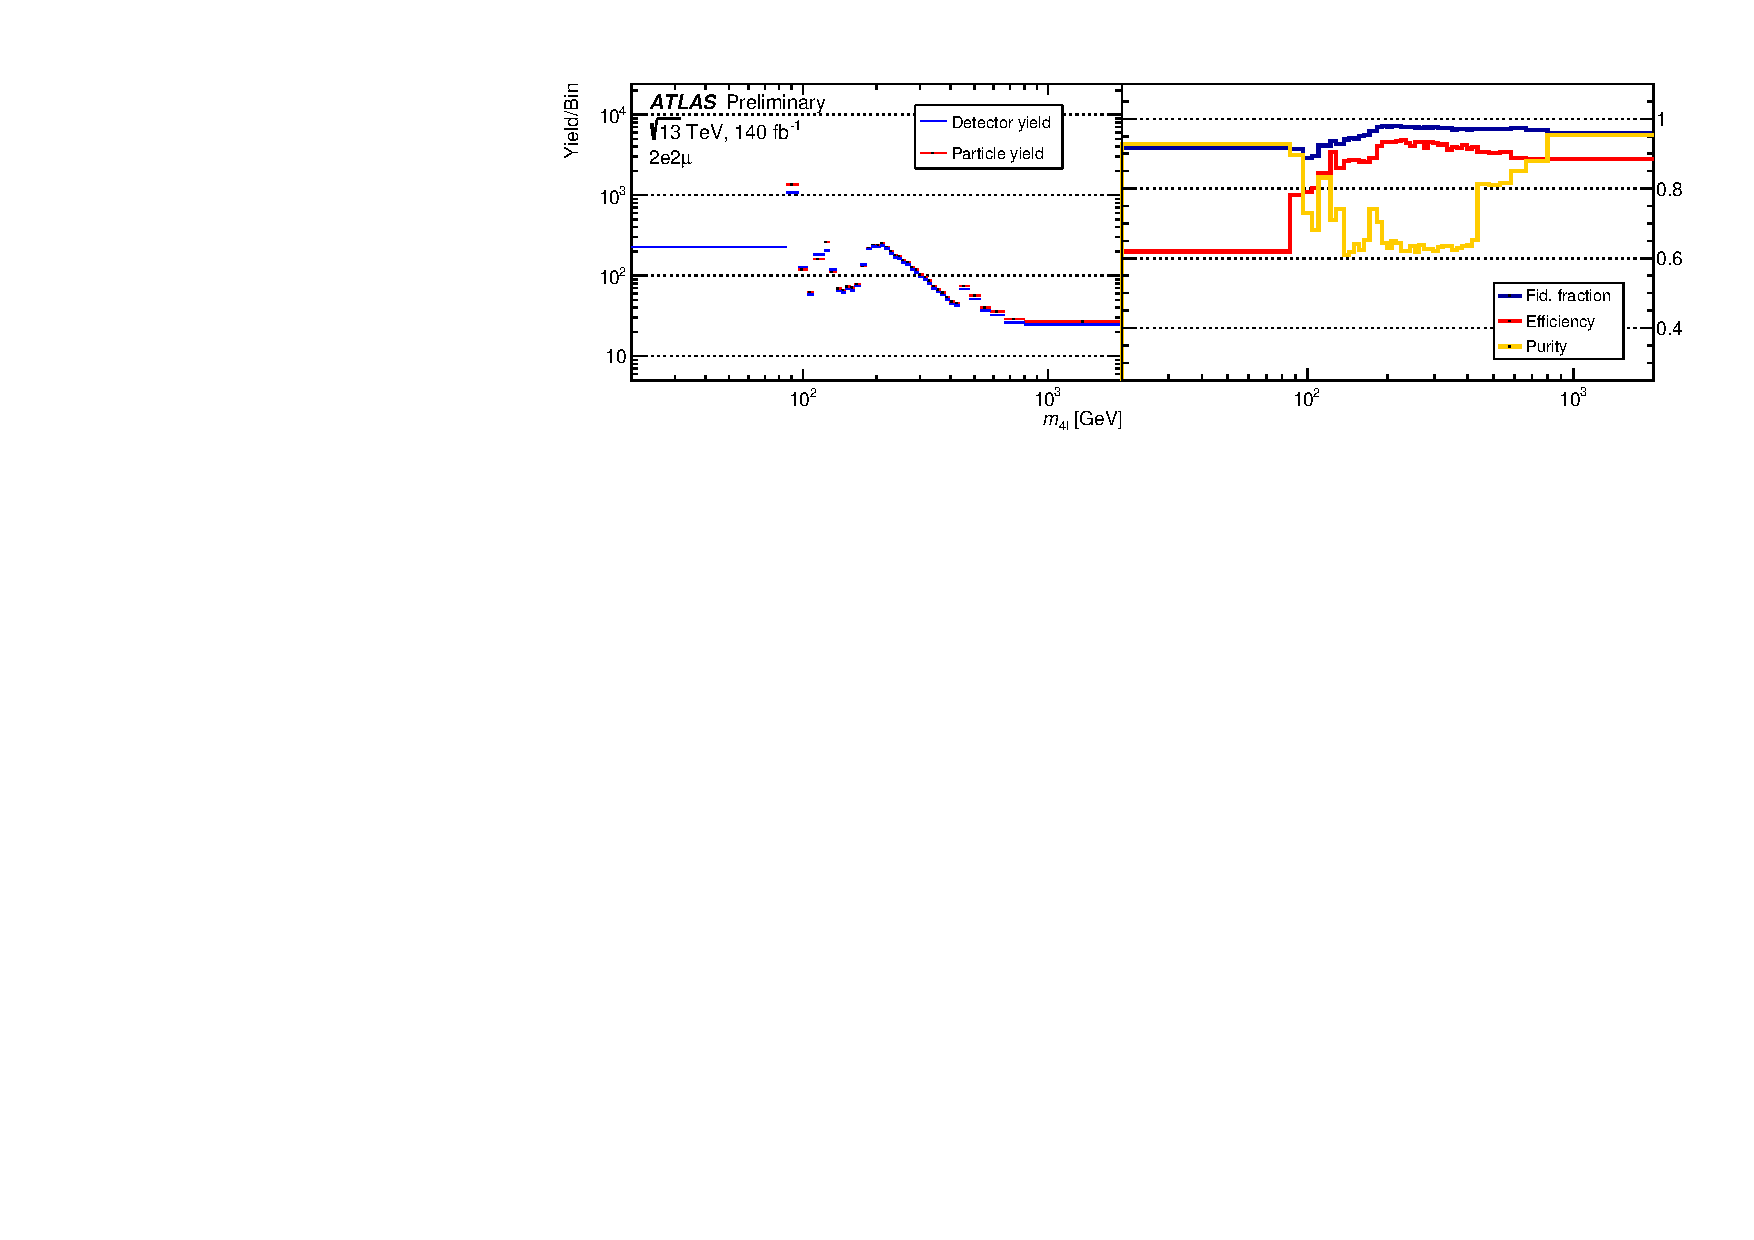
\includegraphics[width = 0.75\textwidth]{Figures/m4l/UnfoldingStudies/v014_inputs/m4l_event_type1-3inputs.pdf}
    \end{subfigure}
    \caption{In the left-hand panels, the number of predicted events passing the reconstruction- and fiducial- level selections are displayed as the detector yield and particle yield, respectively. The right-hand panel shows the efficiency, fiducial purity and fiducial fraction. All variables are plotted as a function of the \mFourL bins, in the $4e$, $4\mu$ and $2e2\mu$ flavour channels from top to bottom.
    \label{fig:chunf}}
\end{figure}  

\FloatBarrier
\clearpage

%%double differentials in coarse mass bins
%Z variables
\begin{figure}[htb]
    \centering 
    \begin{subfigure}{.99\textwidth}\centering
        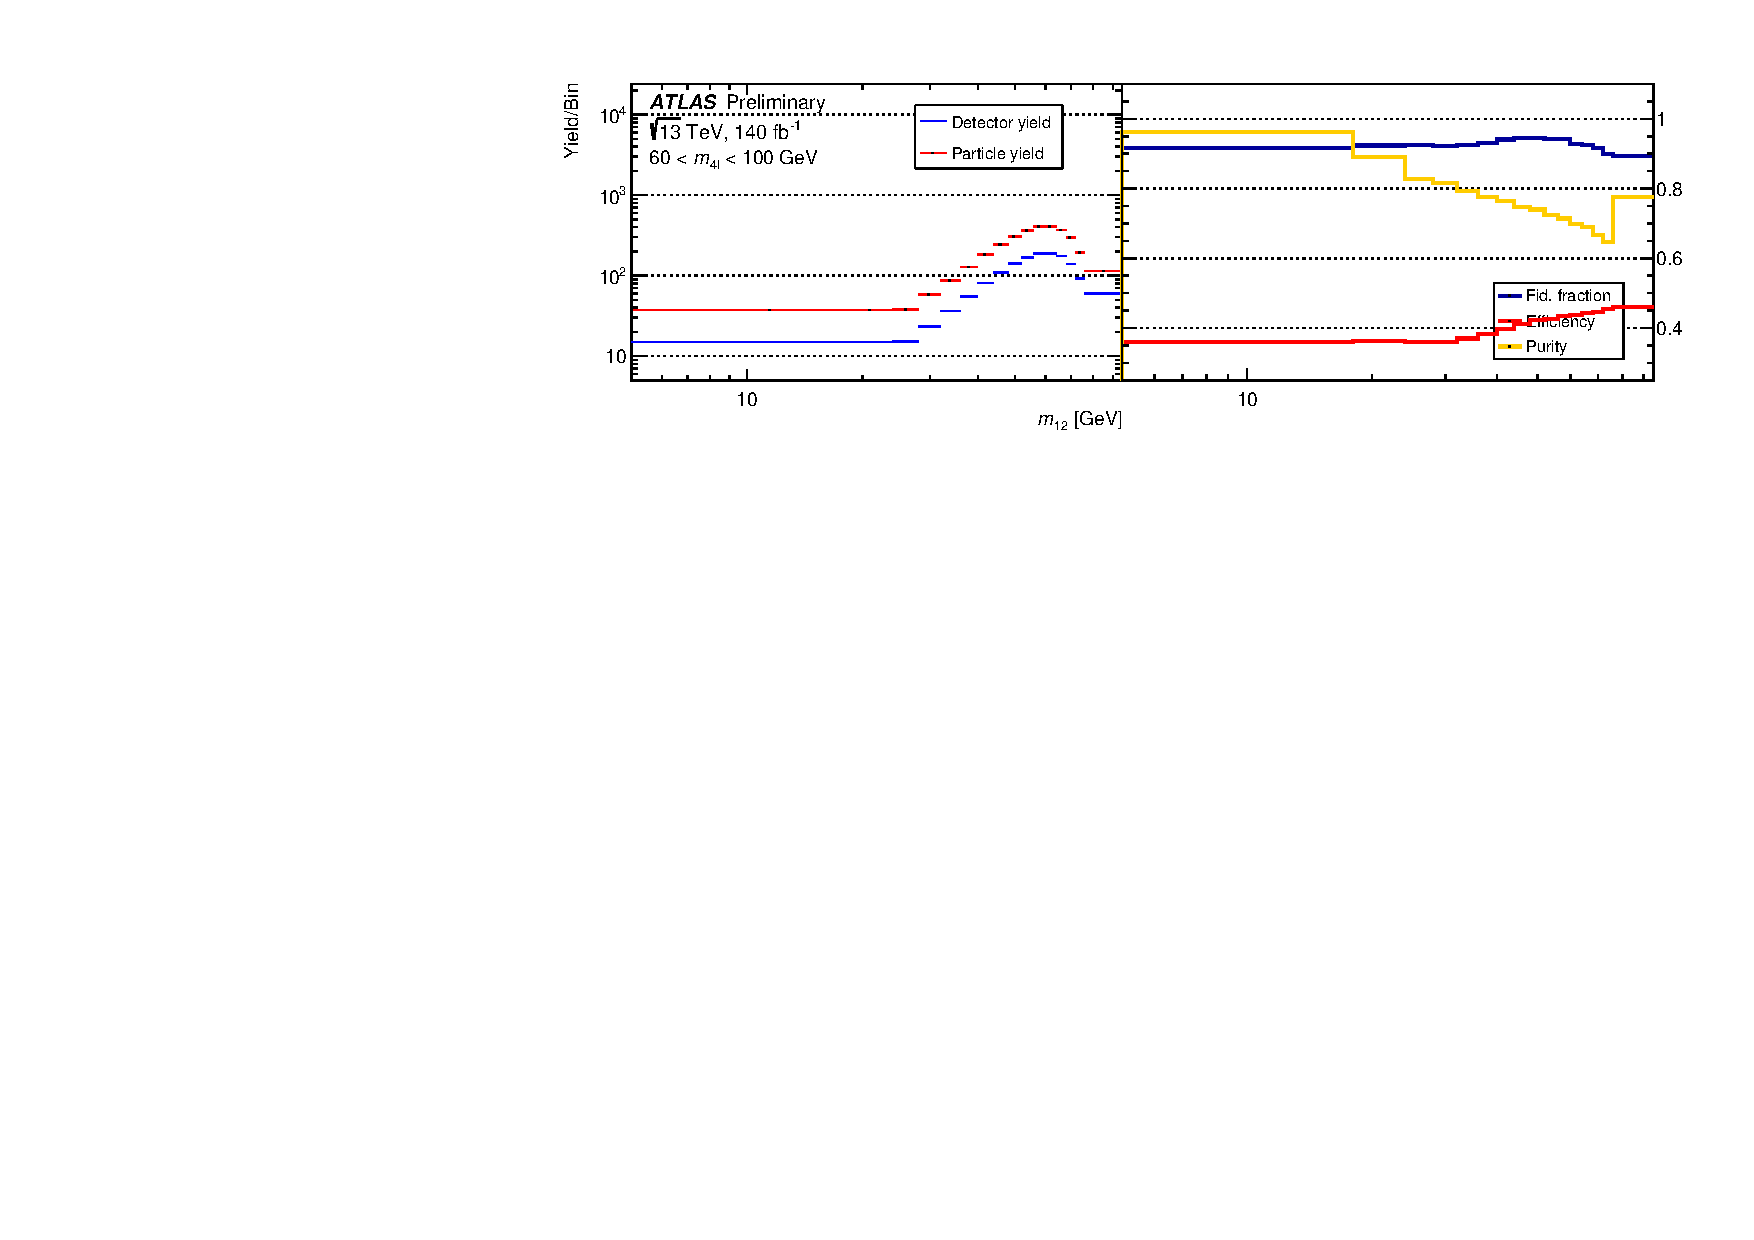
\includegraphics[width = 0.75\textwidth]{Figures/m4l/UnfoldingStudies/v014_inputs/m12_m4l60-100inputs.pdf}
    \end{subfigure}
    \begin{subfigure}{.99\textwidth}\centering
        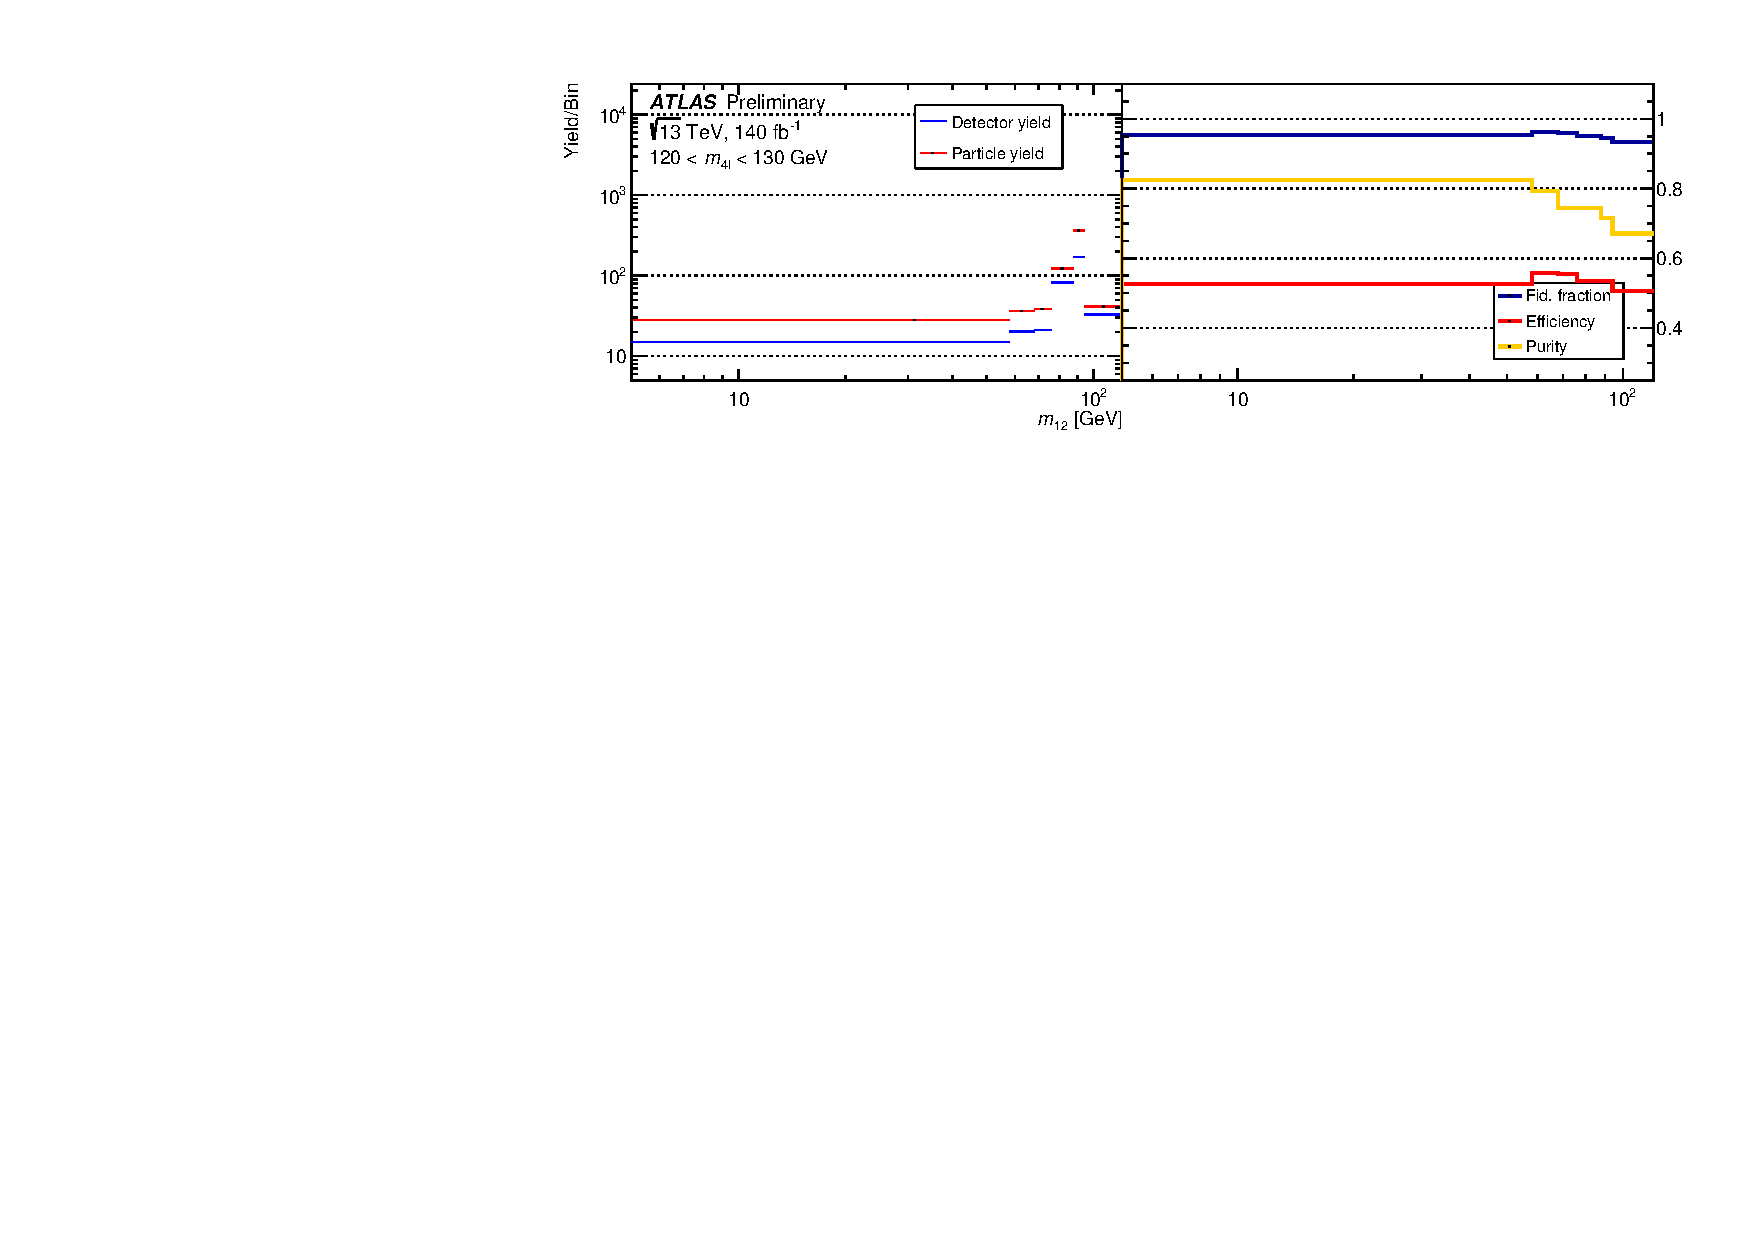
\includegraphics[width = 0.75\textwidth]{Figures/m4l/UnfoldingStudies/v014_inputs/m12_m4l120-130inputs.pdf}
    \end{subfigure}
    \begin{subfigure}{.99\textwidth}\centering
        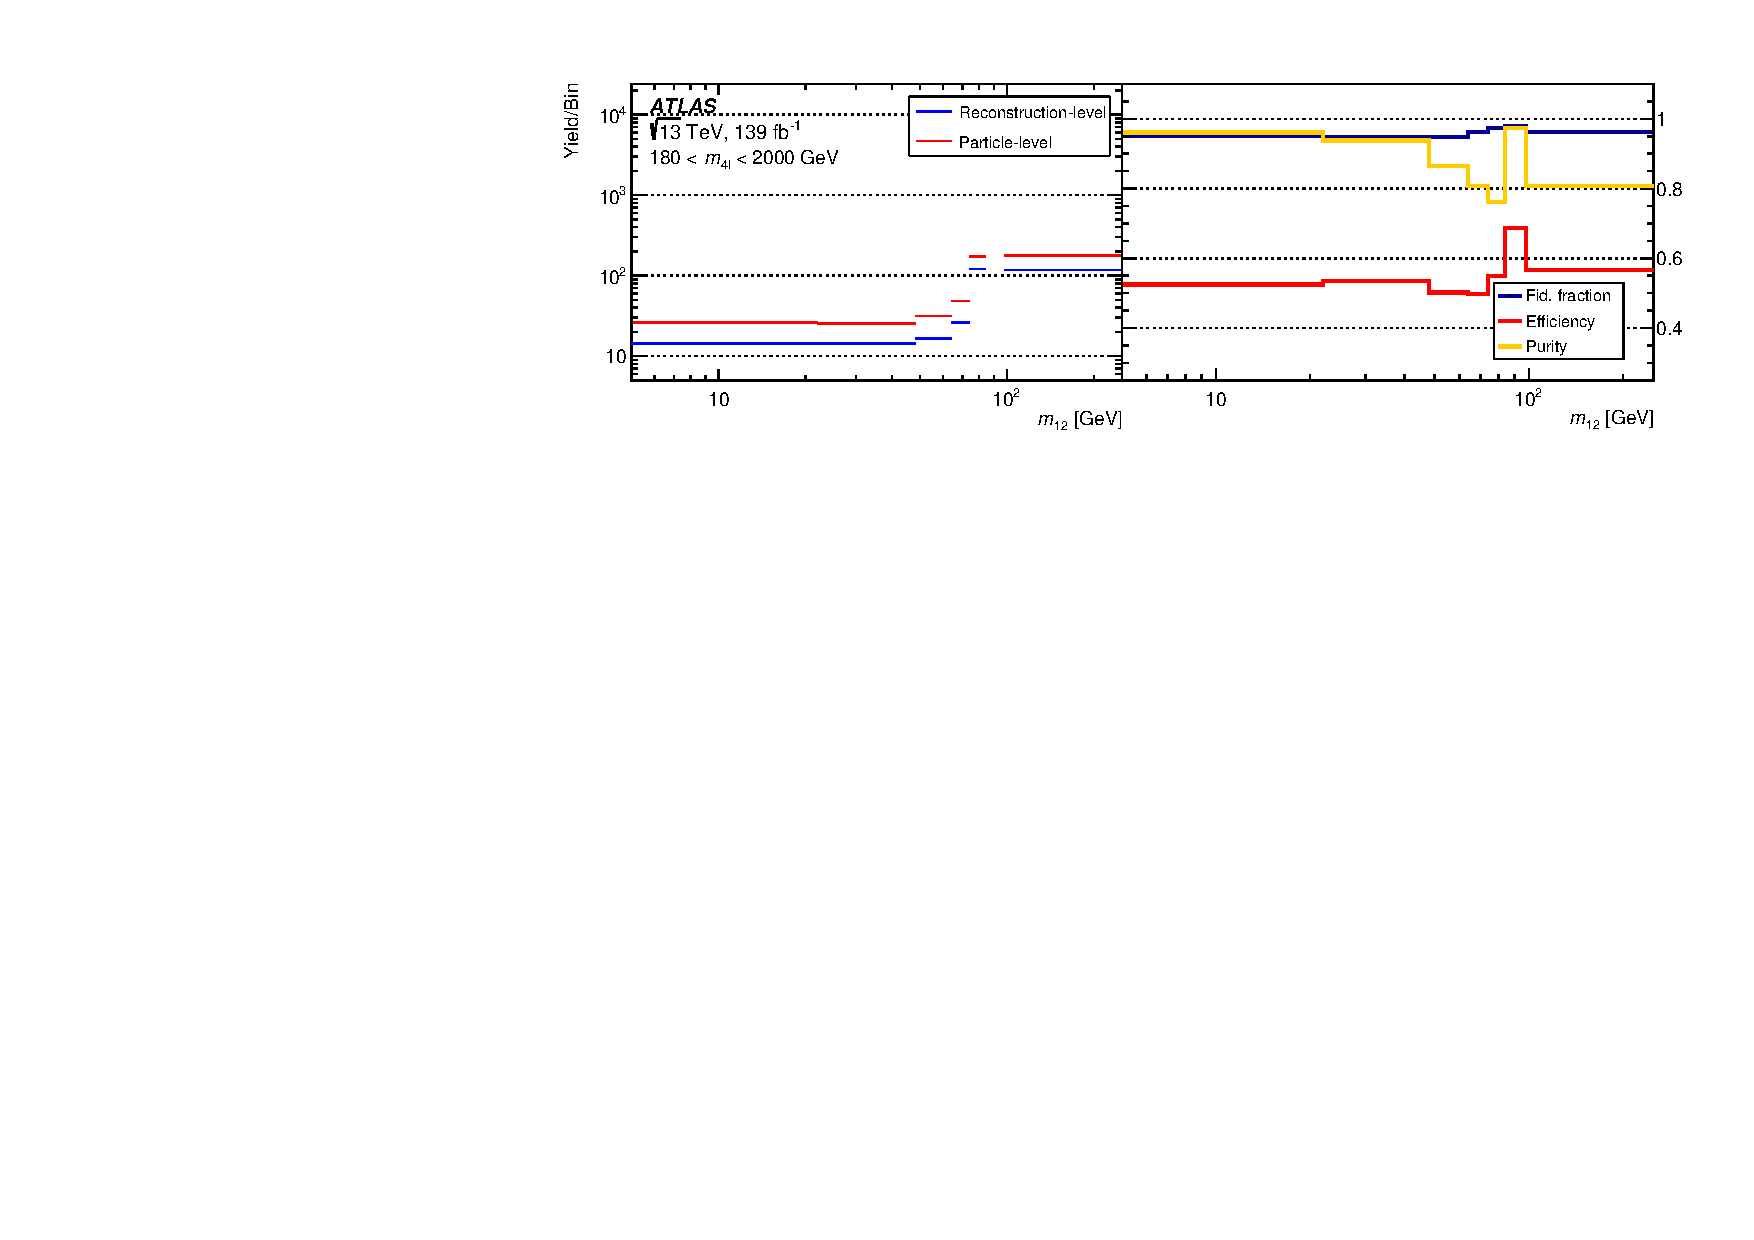
\includegraphics[width = 0.75\textwidth]{Figures/m4l/UnfoldingStudies/v014_inputs/m12_m4l180-2000inputs.pdf}
    \end{subfigure}
    \begin{subfigure}{.99\textwidth}\centering
        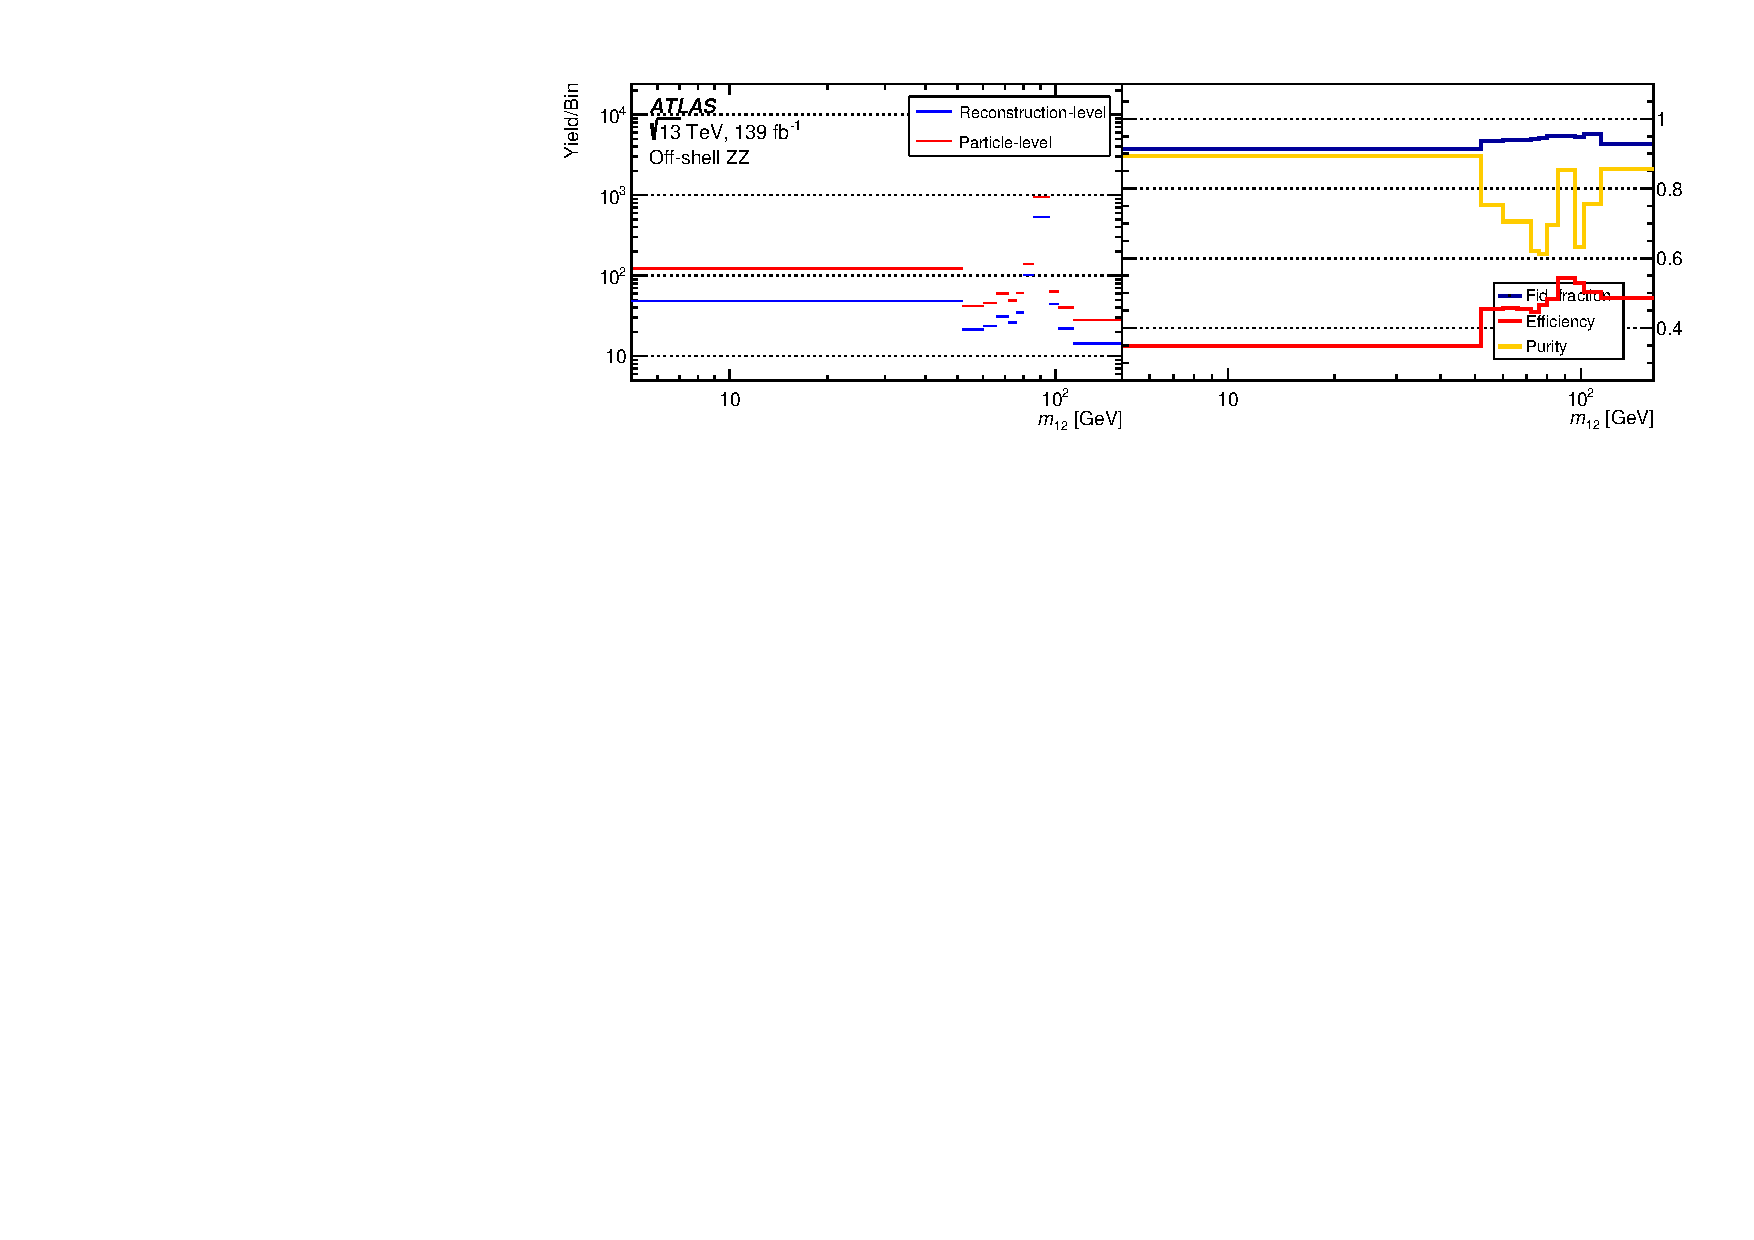
\includegraphics[width = 0.75\textwidth]{Figures/m4l/UnfoldingStudies/v014_inputs/m12_m4loffshellinputs.pdf}
    \end{subfigure}
    \caption{In the left-hand panels, the number of predicted events passing the reconstruction- and fiducial- level selections are displayed as the detector yield and particle yield, respectively. The right-hand panel shows the efficiency, fiducial purity and fiducial fraction. All variables are plotted as a function of the \mZOne bins, in slices of the \mFourL variable which are stacked and labelled with the included \mFourL range.
    \label{fig:mZ1unf}}
\end{figure}  

\FloatBarrier
\clearpage

\begin{figure}[htb]
    \centering 
    \begin{subfigure}{.99\textwidth}\centering
        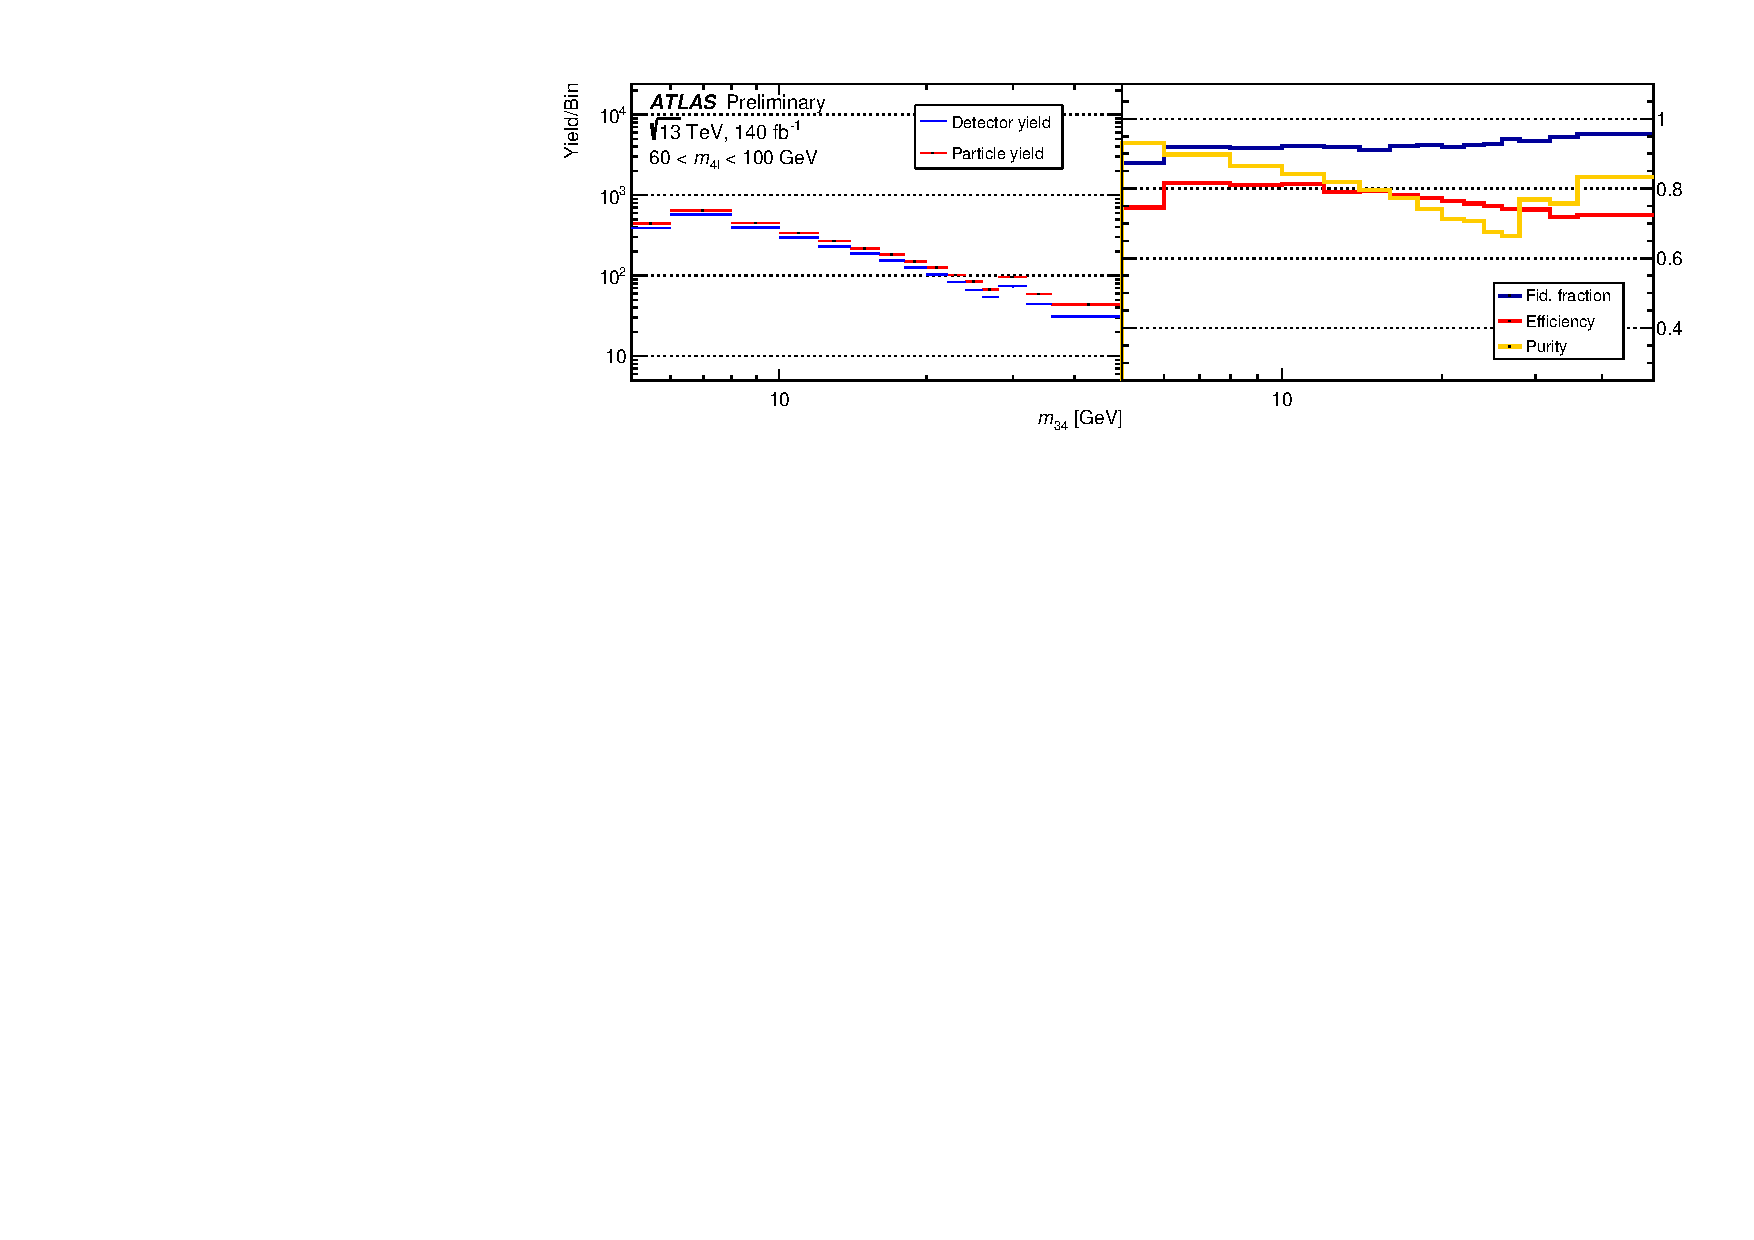
\includegraphics[width = 0.75\textwidth]{Figures/m4l/UnfoldingStudies/v014_inputs/m34_m4l60-100inputs.pdf}
    \end{subfigure}
    \begin{subfigure}{.99\textwidth}\centering
        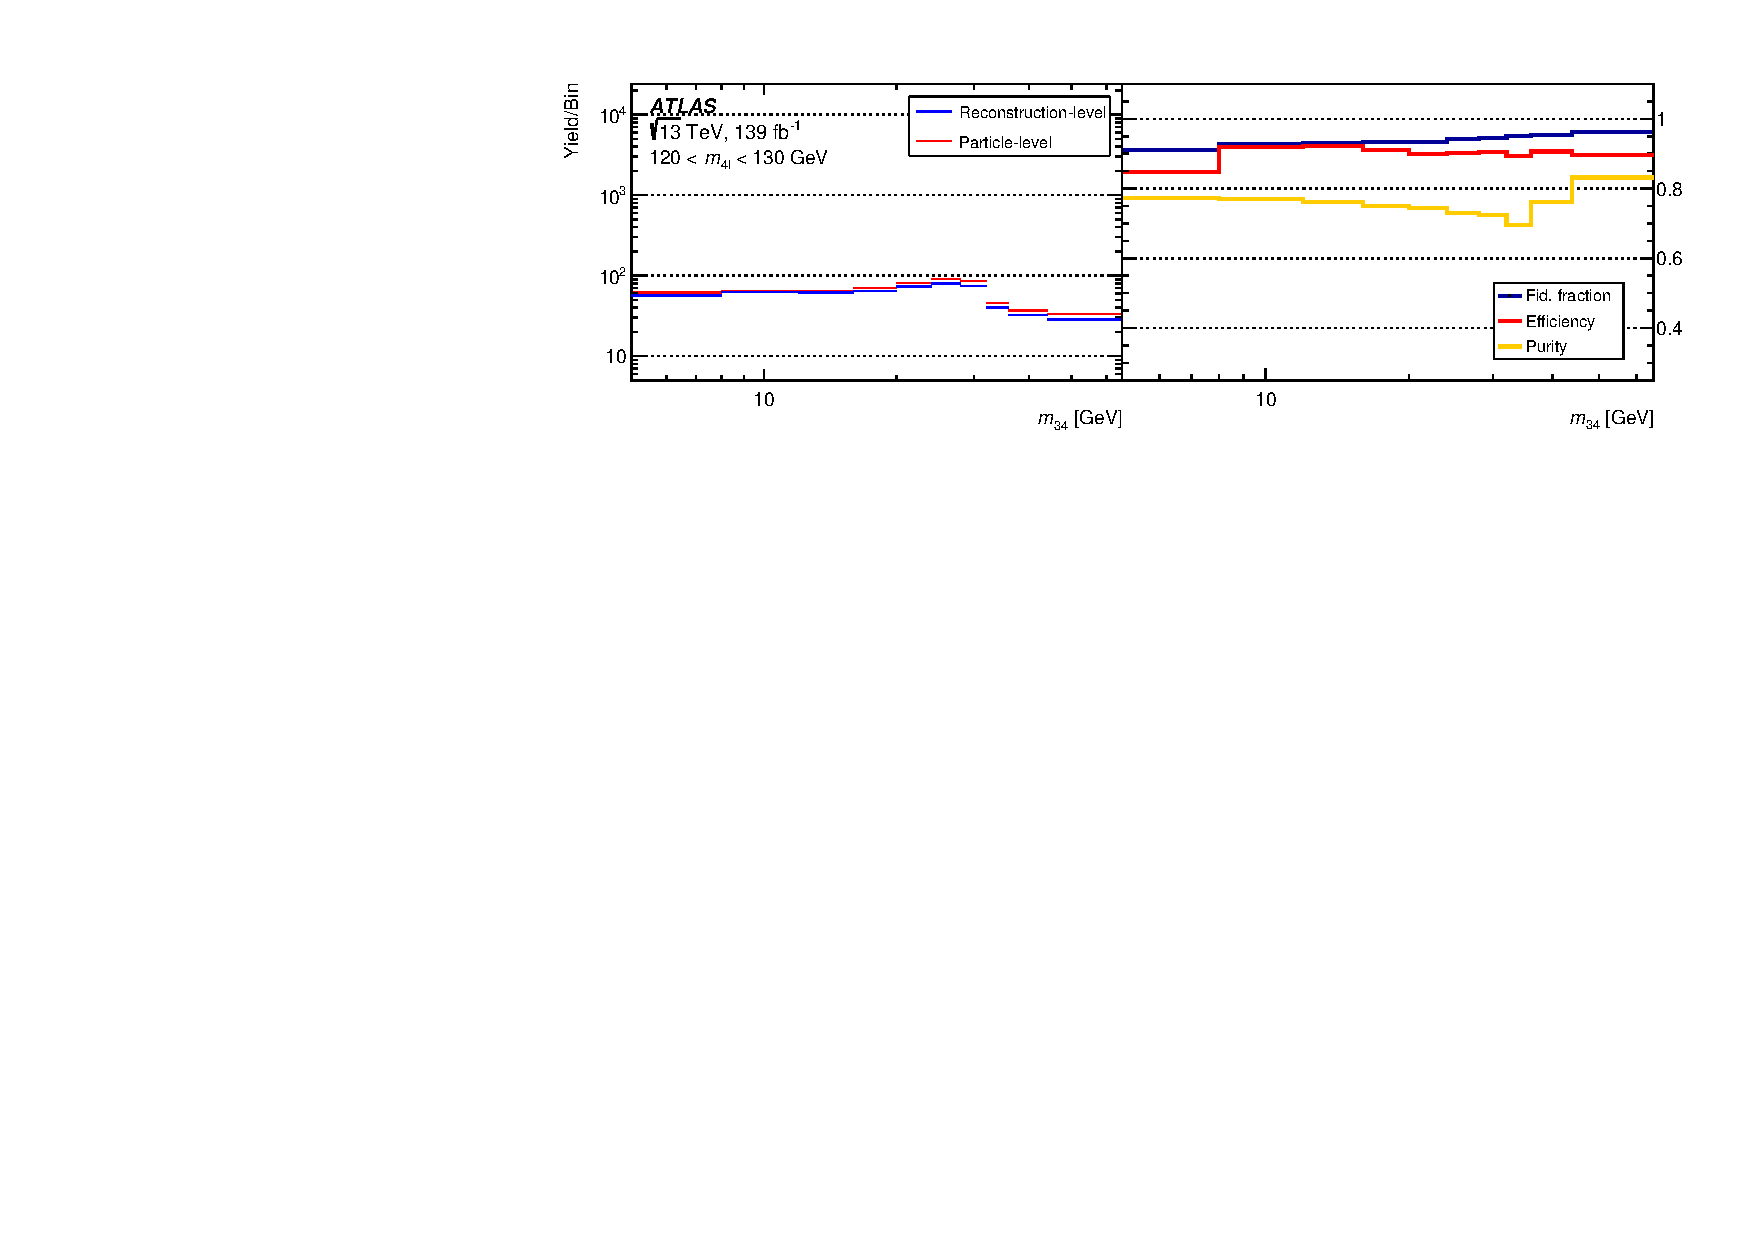
\includegraphics[width = 0.75\textwidth]{Figures/m4l/UnfoldingStudies/v014_inputs/m34_m4l120-130inputs.pdf}
    \end{subfigure}
    \begin{subfigure}{.99\textwidth}\centering
        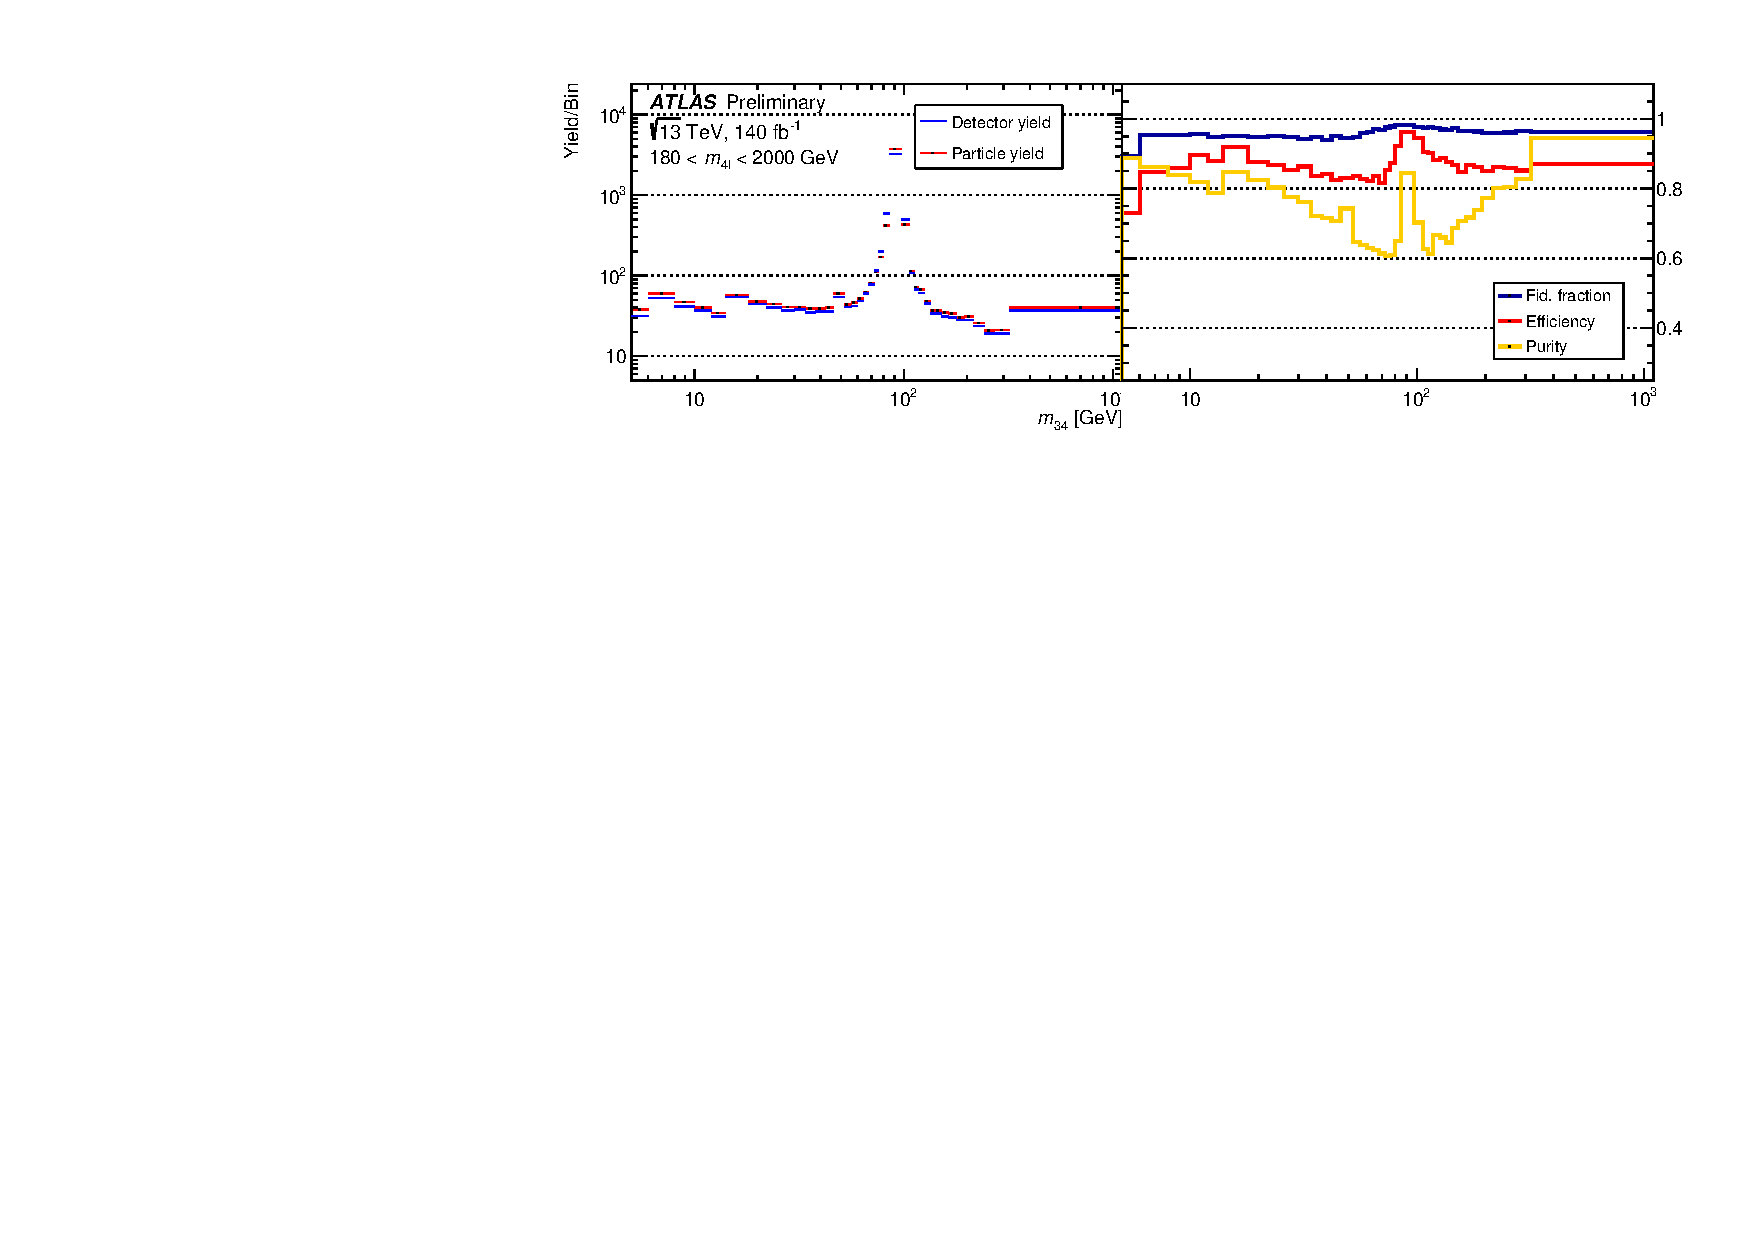
\includegraphics[width = 0.75\textwidth]{Figures/m4l/UnfoldingStudies/v014_inputs/m34_m4l180-2000inputs.pdf}
    \end{subfigure}
    \begin{subfigure}{.99\textwidth}\centering
        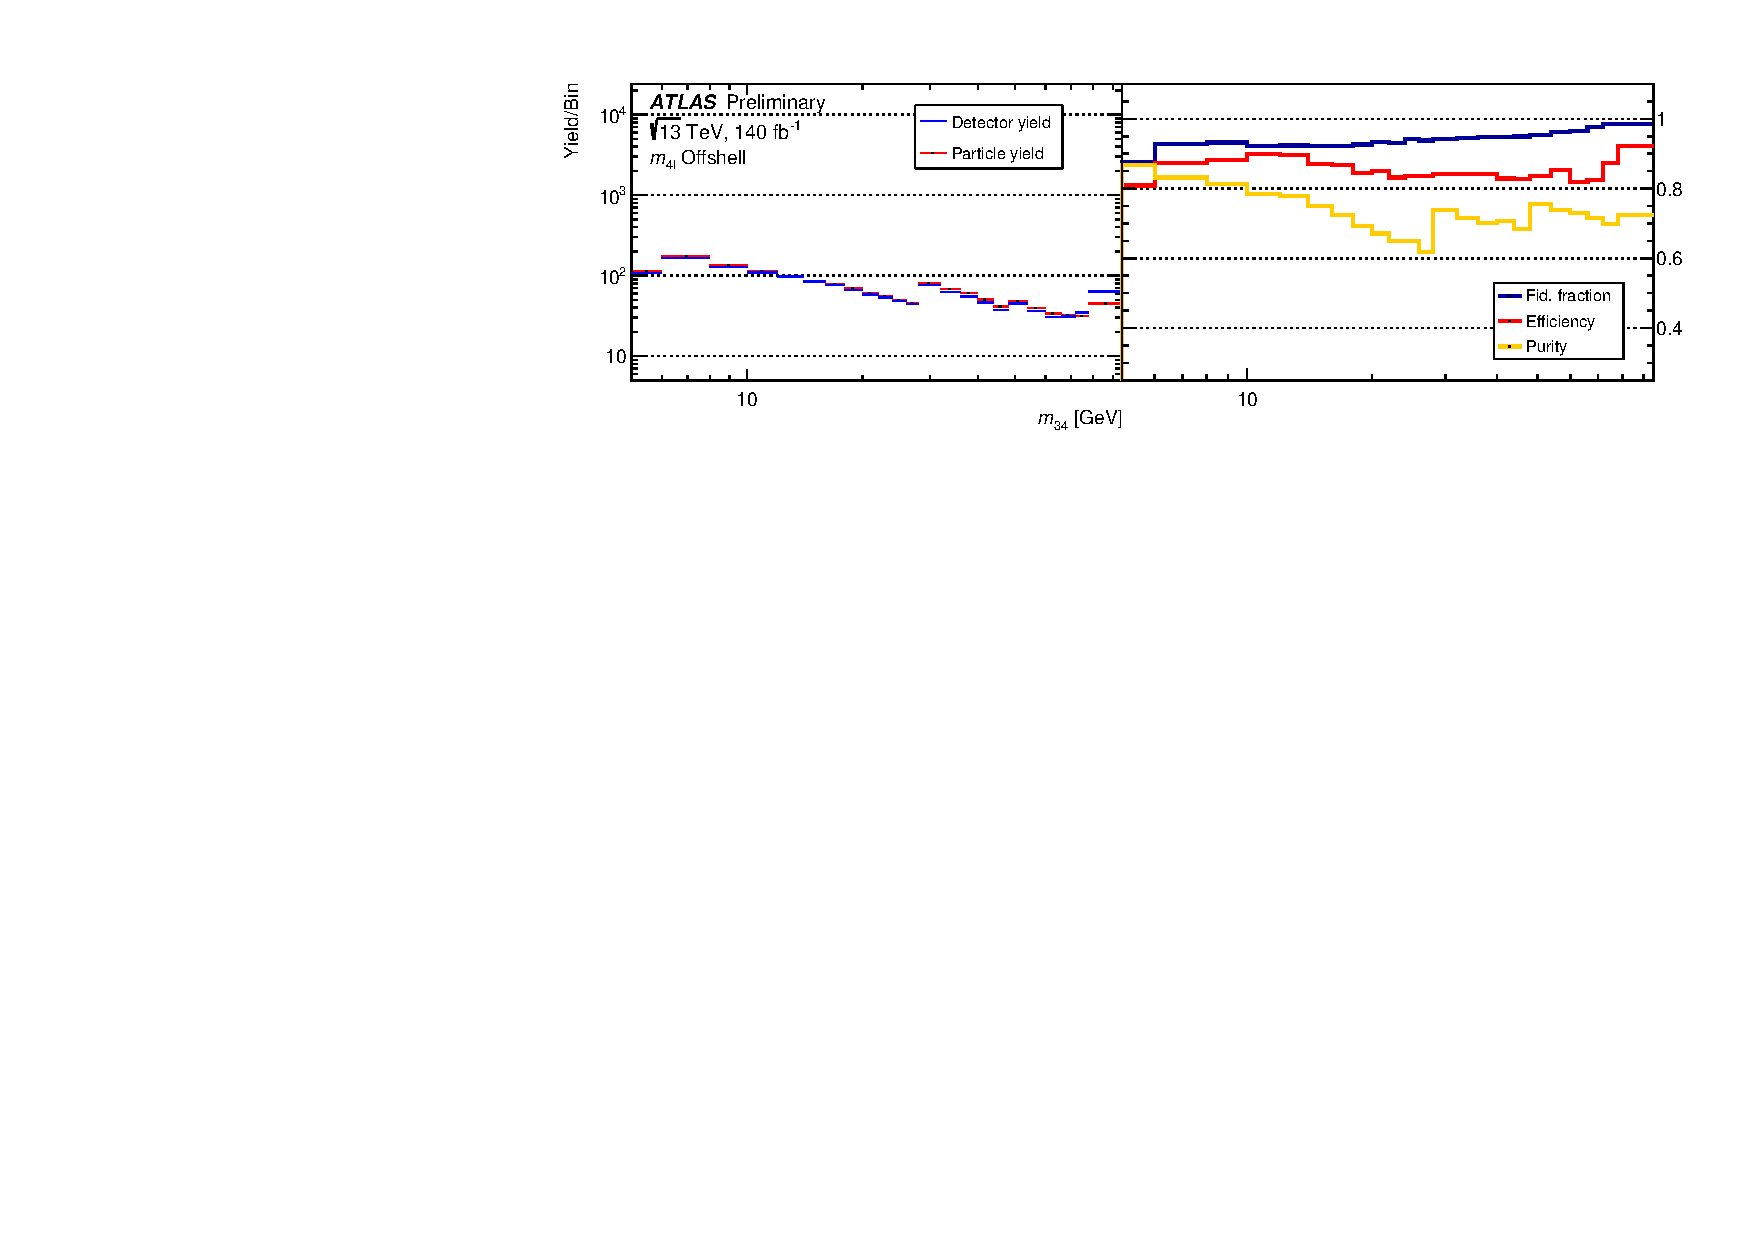
\includegraphics[width = 0.75\textwidth]{Figures/m4l/UnfoldingStudies/v014_inputs/m34_m4loffshellinputs.pdf}
    \end{subfigure}
    \caption{In the left-hand panels, the number of predicted events passing the reconstruction- and fiducial- level selections are displayed as the detector yield and particle yield, respectively. The right-hand panel shows the efficiency, fiducial purity and fiducial fraction. All variables are plotted as a function of the \mZTwo bins, in slices of the \mFourL variable which are stacked and labelled with the included \mFourL range.
    \label{fig:mZ2unf}}
\end{figure}  

\FloatBarrier
\clearpage

\begin{figure}[htb]
    \centering 
    \begin{subfigure}{.99\textwidth}\centering
        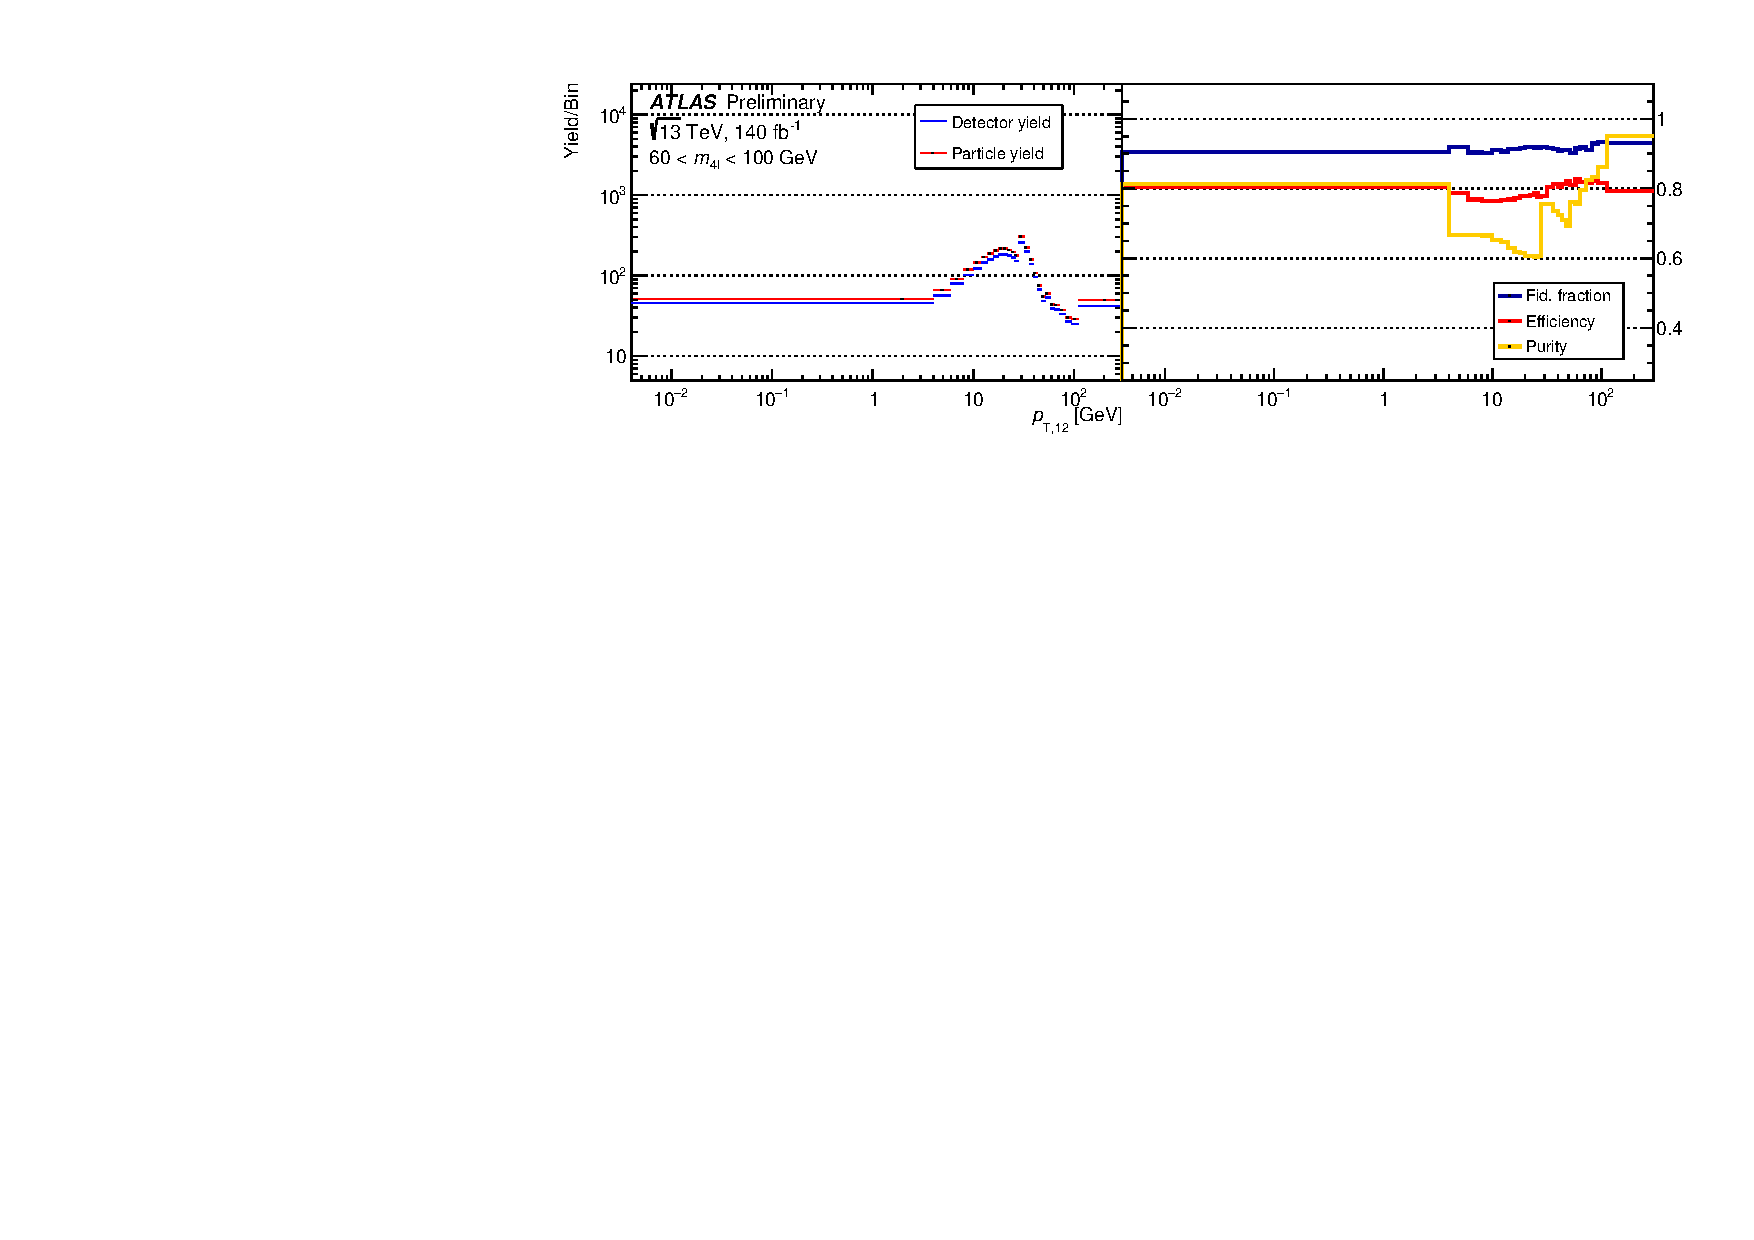
\includegraphics[width = 0.75\textwidth]{Figures/m4l/UnfoldingStudies/v014_inputs/pt12_m4l60-100inputs.pdf}
    \end{subfigure}
    \begin{subfigure}{.99\textwidth}\centering
        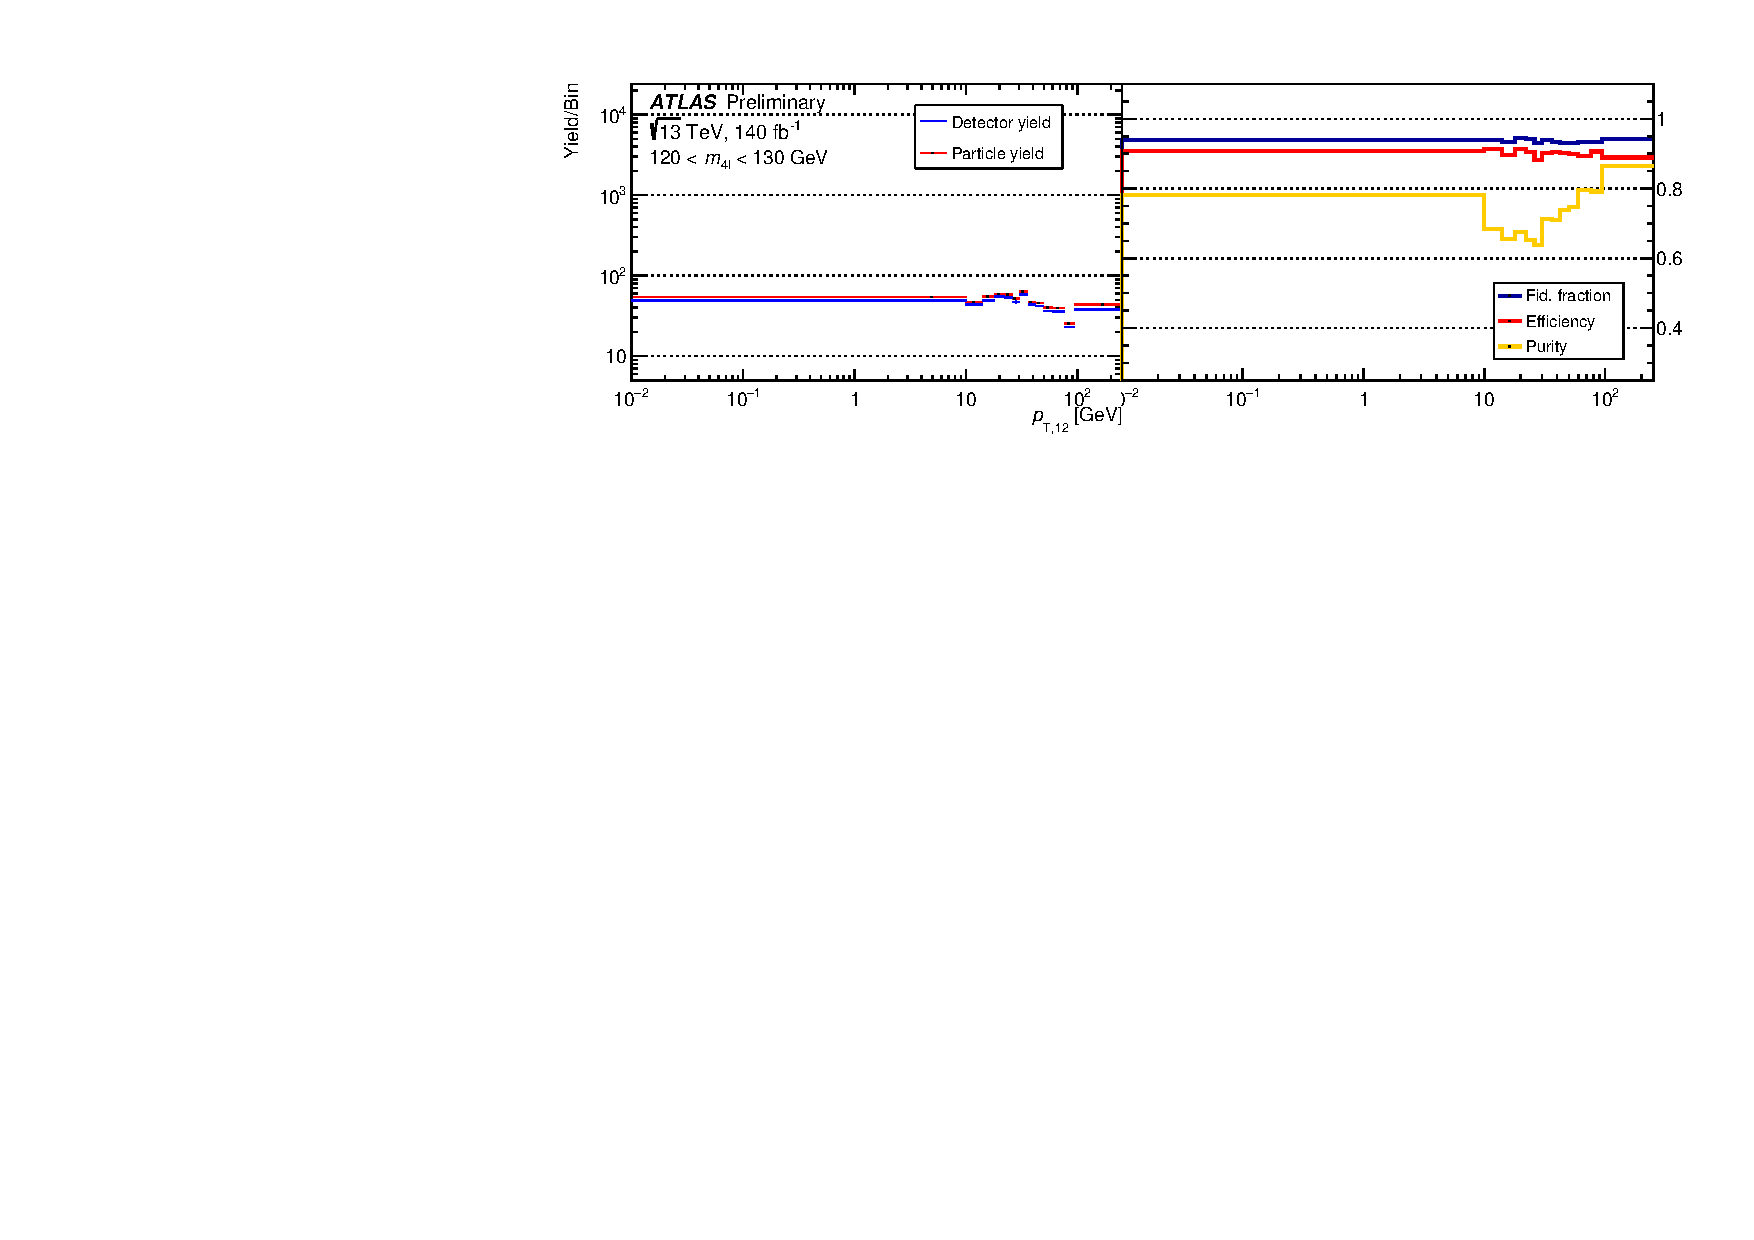
\includegraphics[width = 0.75\textwidth]{Figures/m4l/UnfoldingStudies/v014_inputs/pt12_m4l120-130inputs.pdf}
    \end{subfigure}
    \begin{subfigure}{.99\textwidth}\centering
        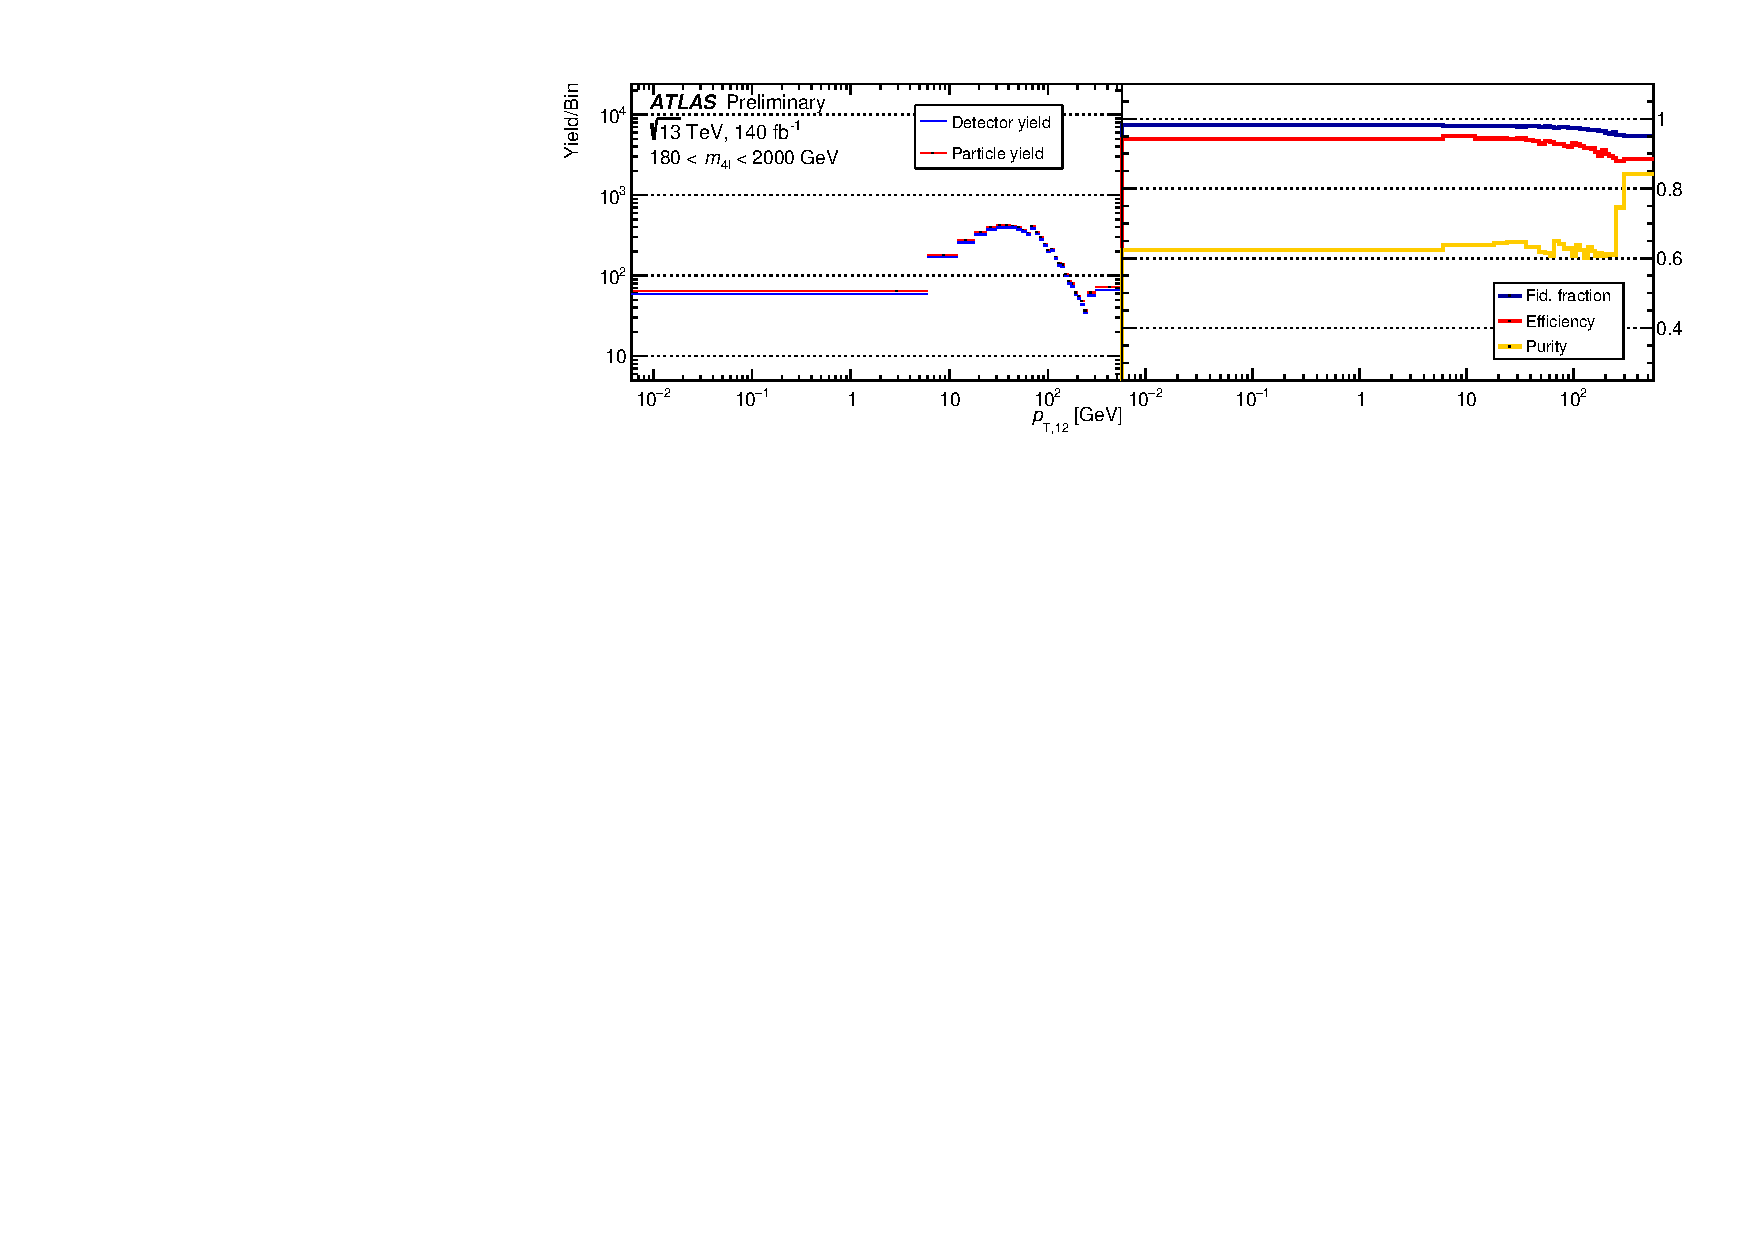
\includegraphics[width = 0.75\textwidth]{Figures/m4l/UnfoldingStudies/v014_inputs/pt12_m4l180-2000inputs.pdf}
    \end{subfigure}
    \begin{subfigure}{.99\textwidth}\centering
        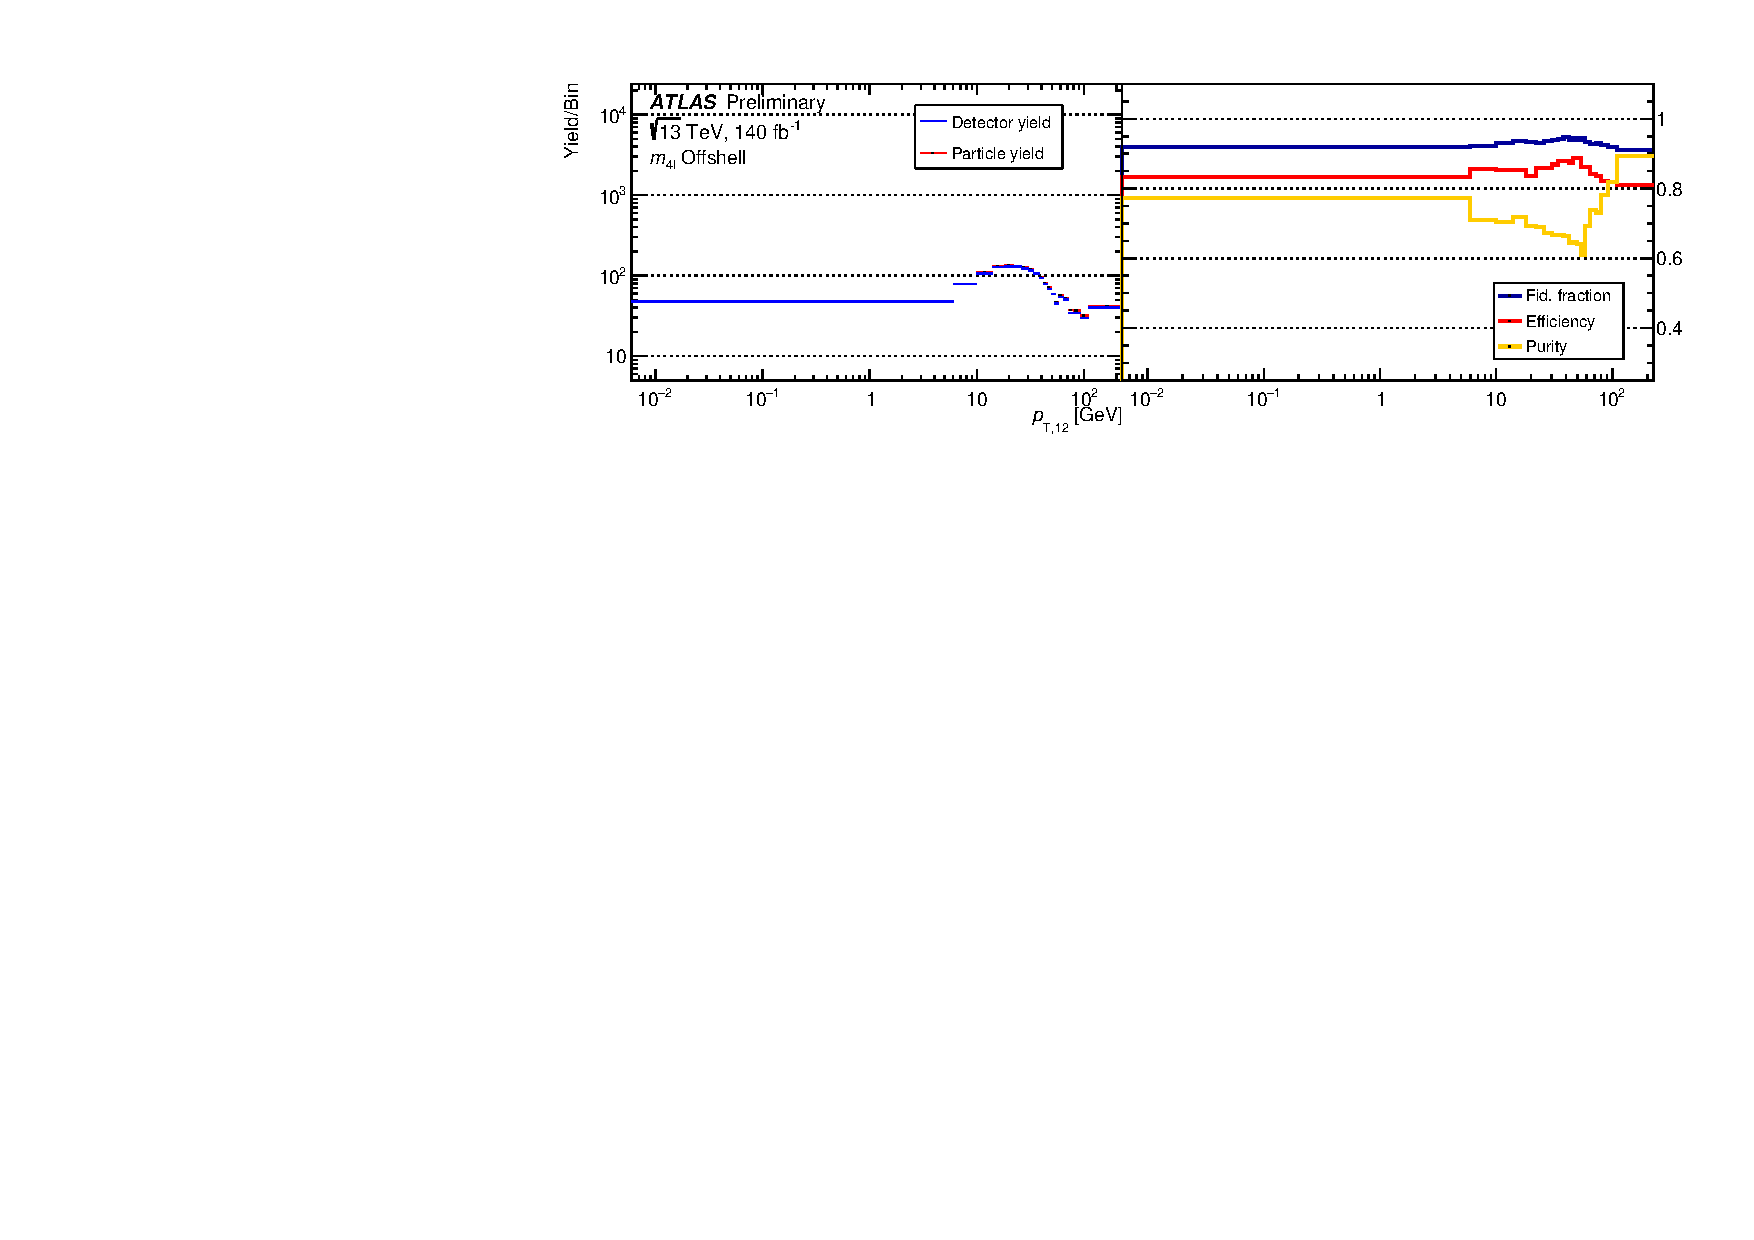
\includegraphics[width = 0.75\textwidth]{Figures/m4l/UnfoldingStudies/v014_inputs/pt12_m4loffshellinputs.pdf}
    \end{subfigure}
    \caption{In the left-hand panels, the number of predicted events passing the reconstruction- and fiducial- level selections are displayed as the detector yield and particle yield, respectively. The right-hand panel shows the efficiency, fiducial purity and fiducial fraction. All variables are plotted as a function of the \ptZOne bins, in slices of the \mFourL variable which are stacked and labelled with the included \mFourL range.
    \label{fig:ptZ1unf}}
\end{figure}  

\FloatBarrier
\clearpage

\begin{figure}[htb]
    \centering 
    \begin{subfigure}{.99\textwidth}\centering
        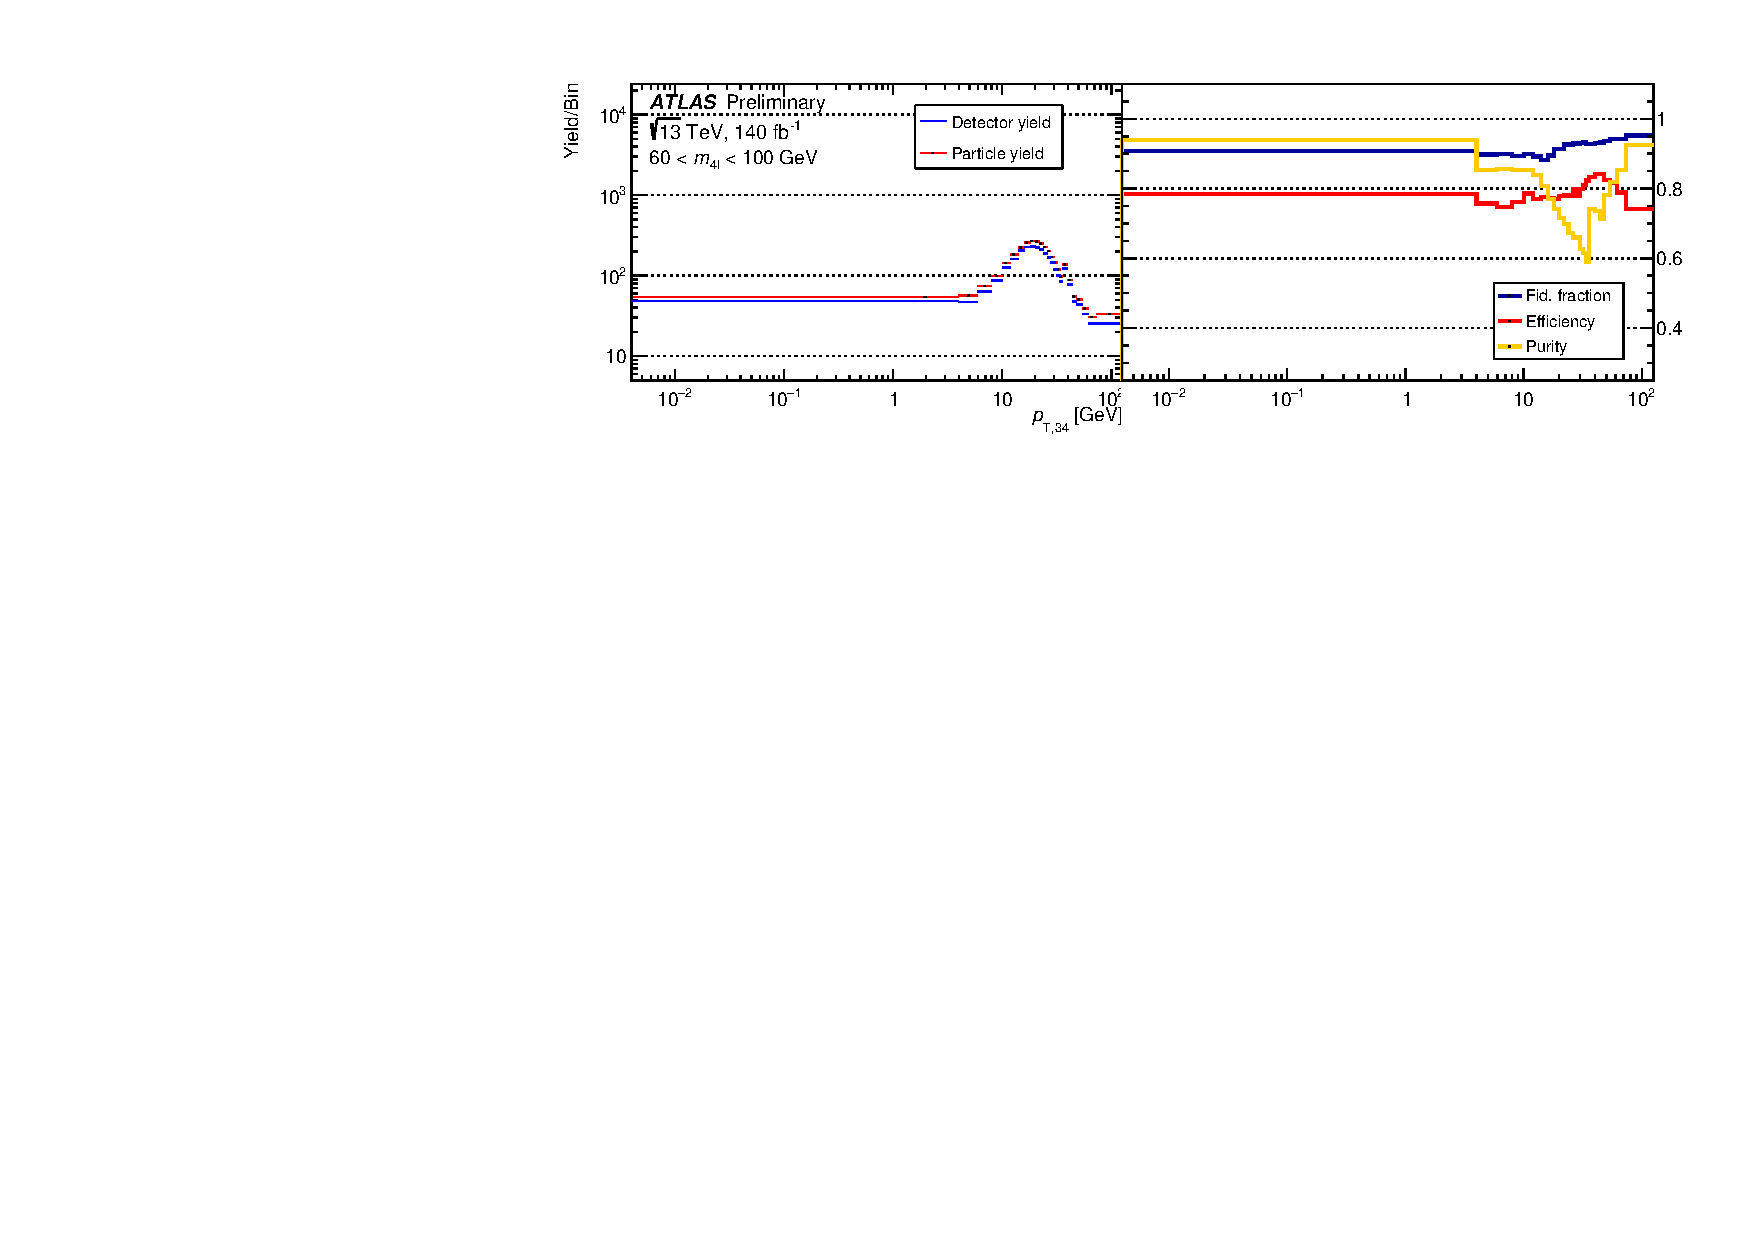
\includegraphics[width = 0.75\textwidth]{Figures/m4l/UnfoldingStudies/v014_inputs/pt34_m4l60-100inputs.pdf}
    \end{subfigure}
    \begin{subfigure}{.99\textwidth}\centering
        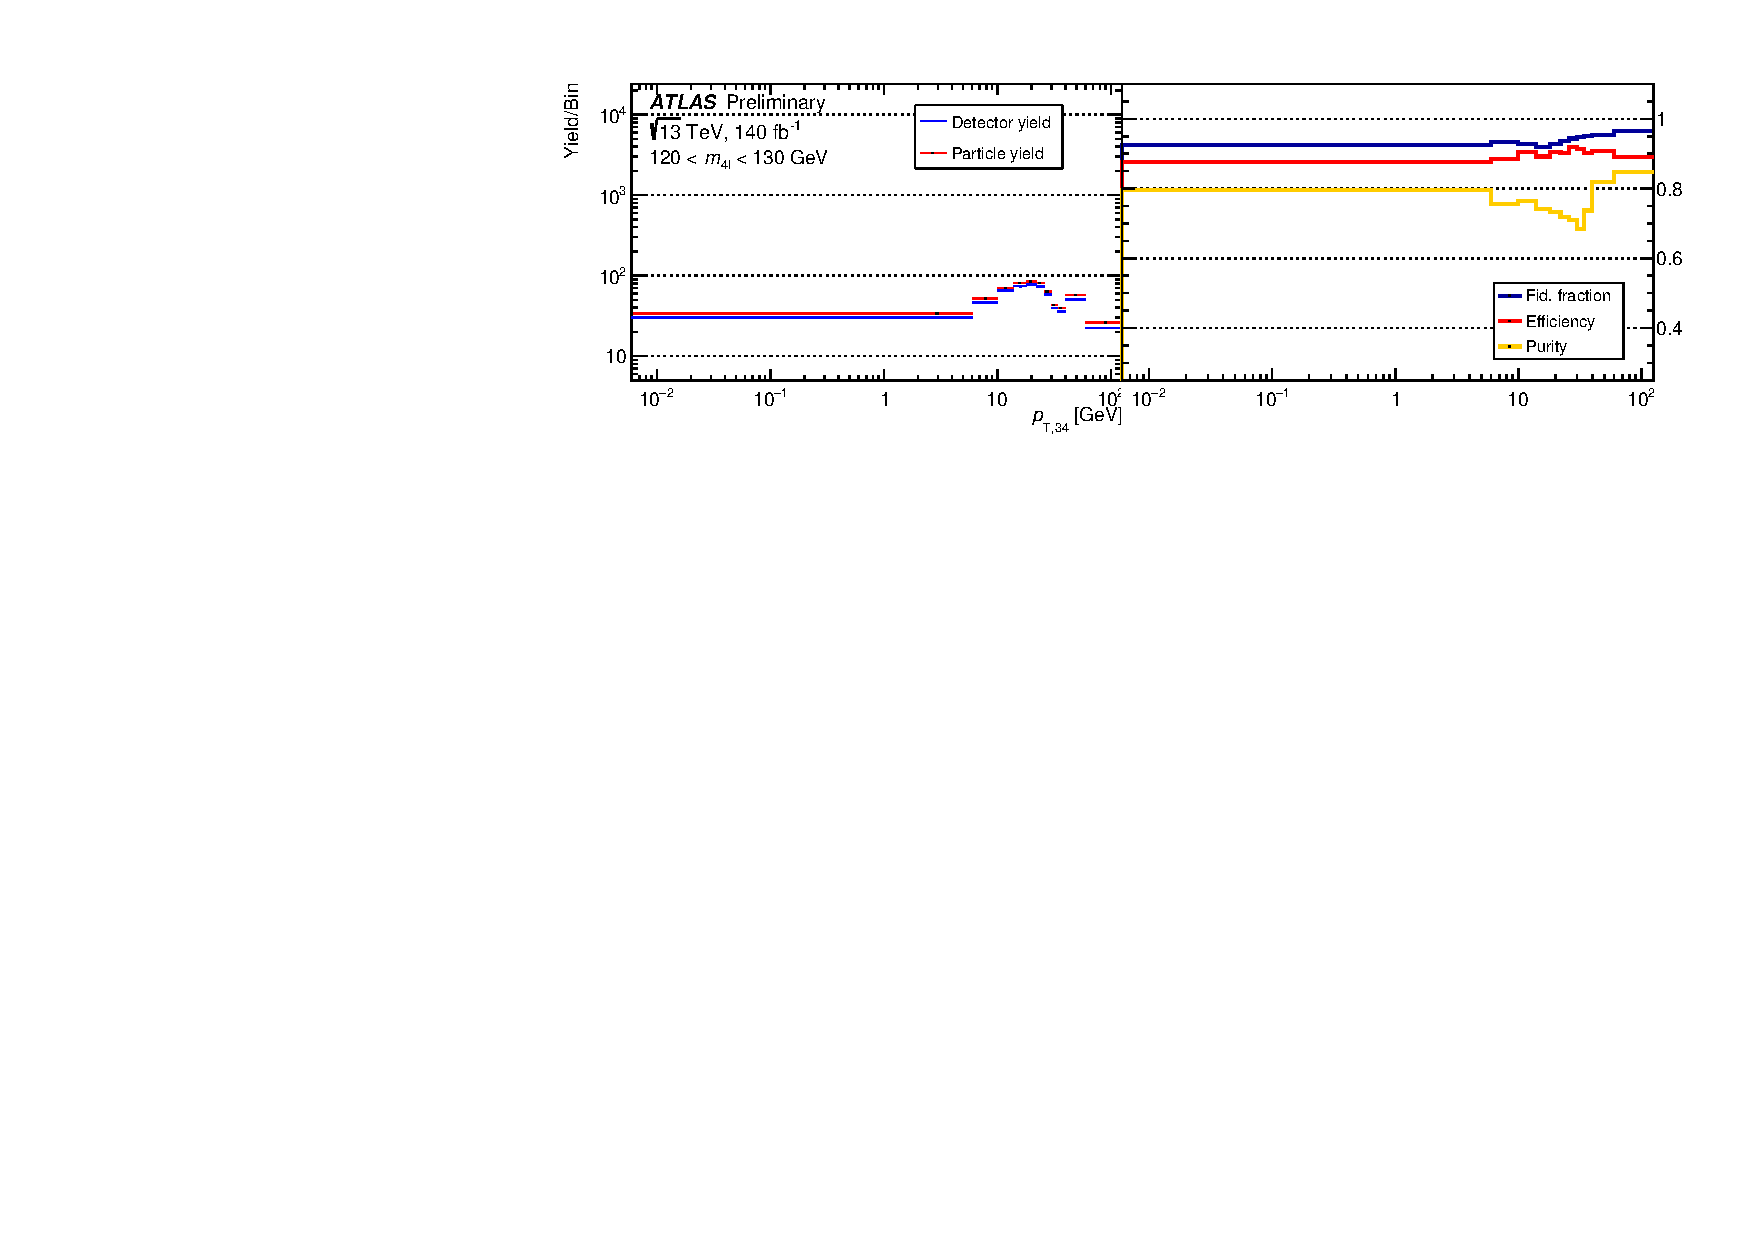
\includegraphics[width = 0.75\textwidth]{Figures/m4l/UnfoldingStudies/v014_inputs/pt34_m4l120-130inputs.pdf}
    \end{subfigure}
    \begin{subfigure}{.99\textwidth}\centering
        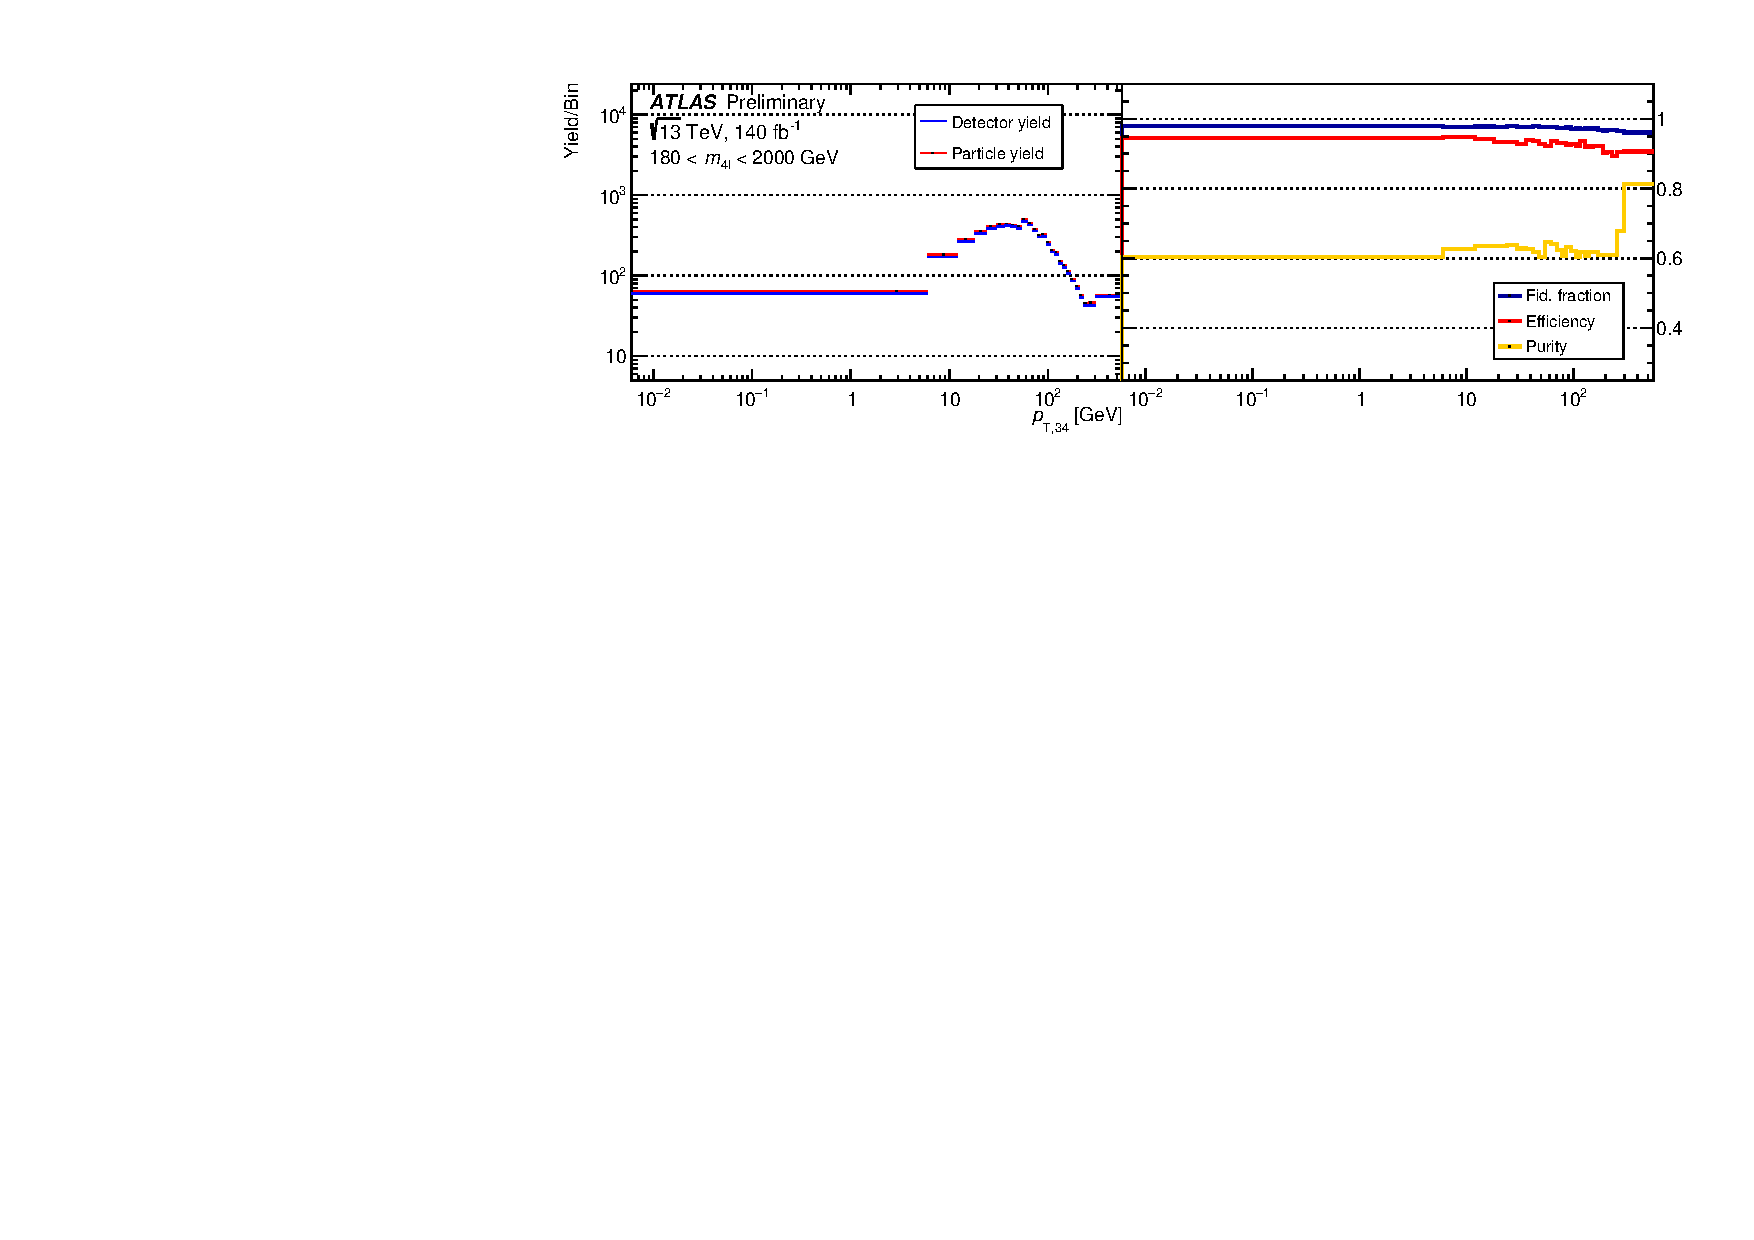
\includegraphics[width = 0.75\textwidth]{Figures/m4l/UnfoldingStudies/v014_inputs/pt34_m4l180-2000inputs.pdf}
    \end{subfigure}
    \begin{subfigure}{.99\textwidth}\centering
        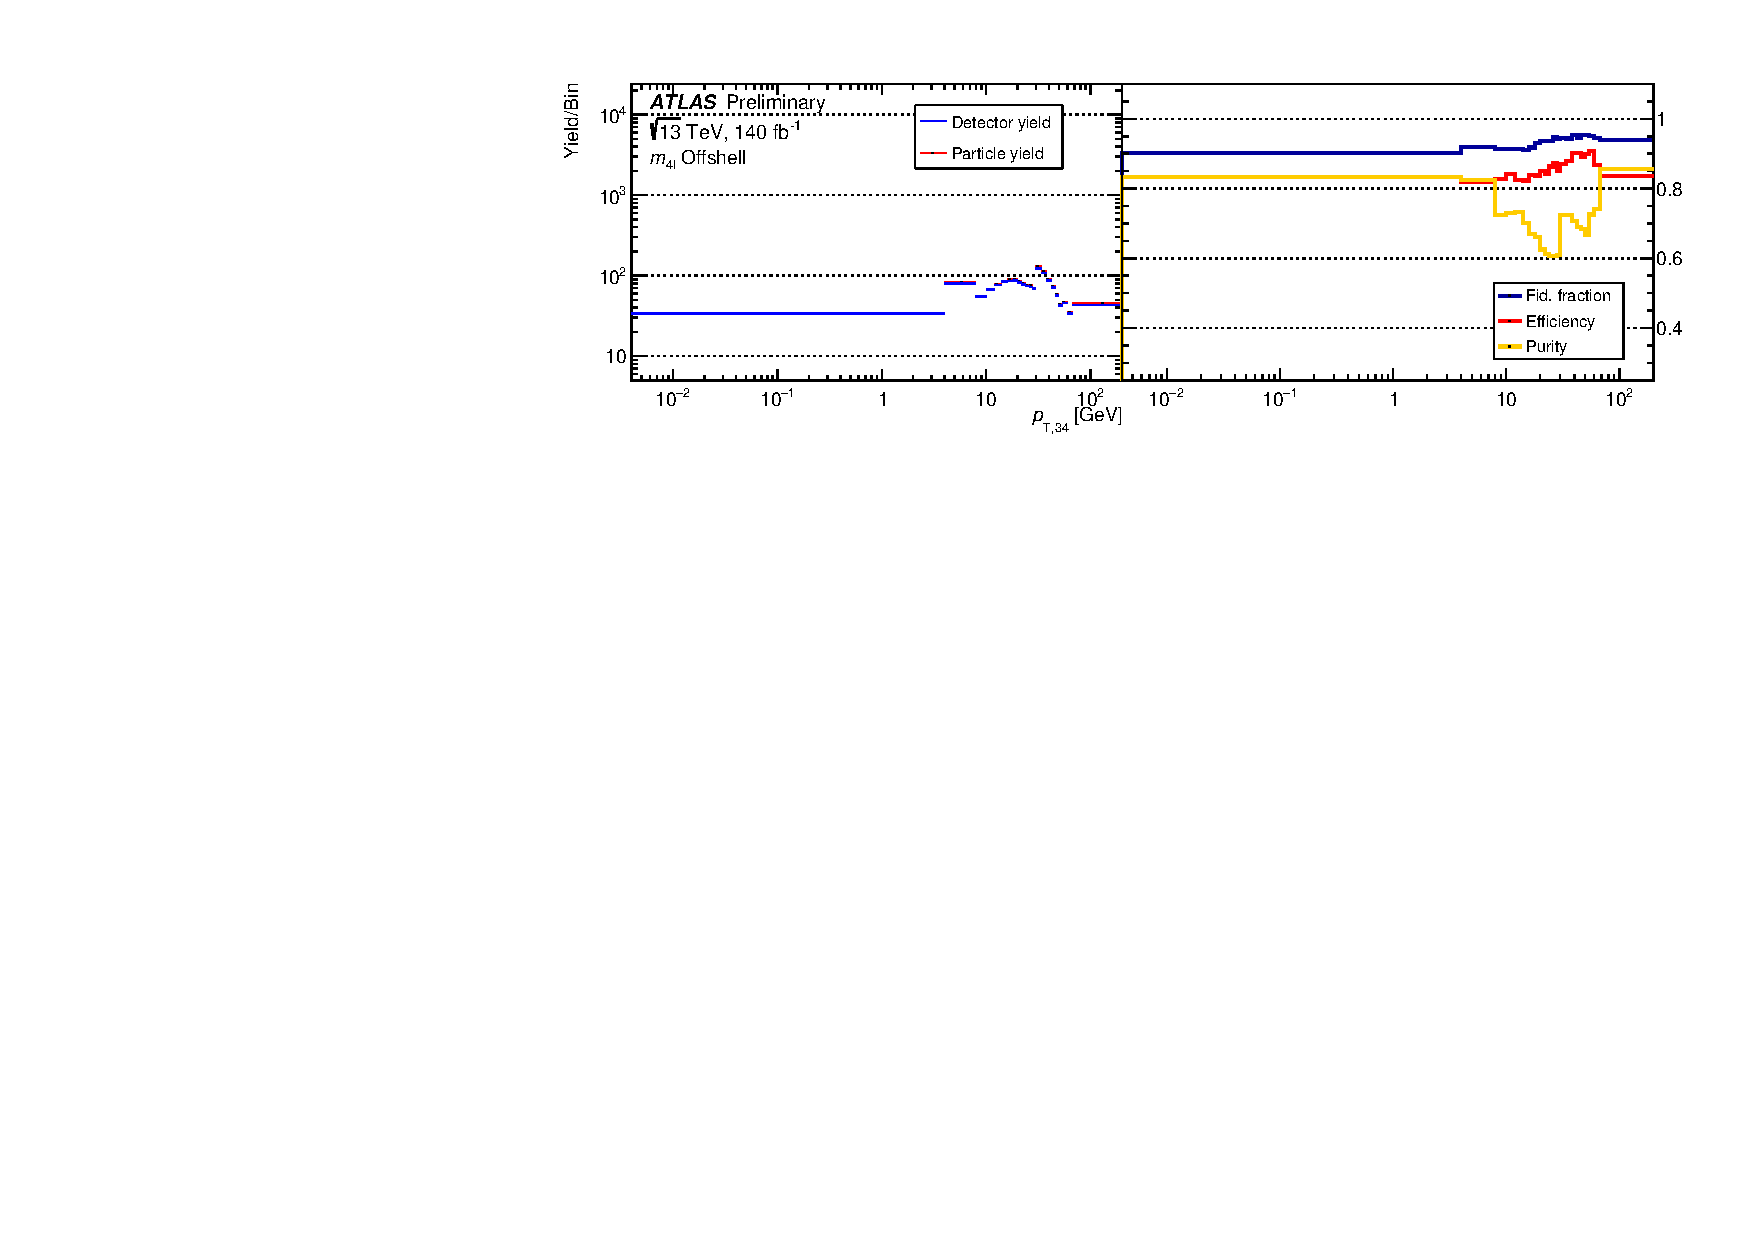
\includegraphics[width = 0.75\textwidth]{Figures/m4l/UnfoldingStudies/v014_inputs/pt34_m4loffshellinputs.pdf}
    \end{subfigure}
    \caption{In the left-hand panels, the number of predicted events passing the reconstruction- and fiducial- level selections are displayed as the detector yield and particle yield, respectively. The right-hand panel shows the efficiency, fiducial purity and fiducial fraction. All variables are plotted as a function of the \ptZTwo bins, in slices of the \mFourL variable which are stacked and labelled with the included \mFourL range.
    \label{fig:ptZ2unf}}
\end{figure}  

\FloatBarrier
\clearpage

%%All angular variables
\begin{figure}[htb]
    \centering 
    \begin{subfigure}{.99\textwidth}\centering
        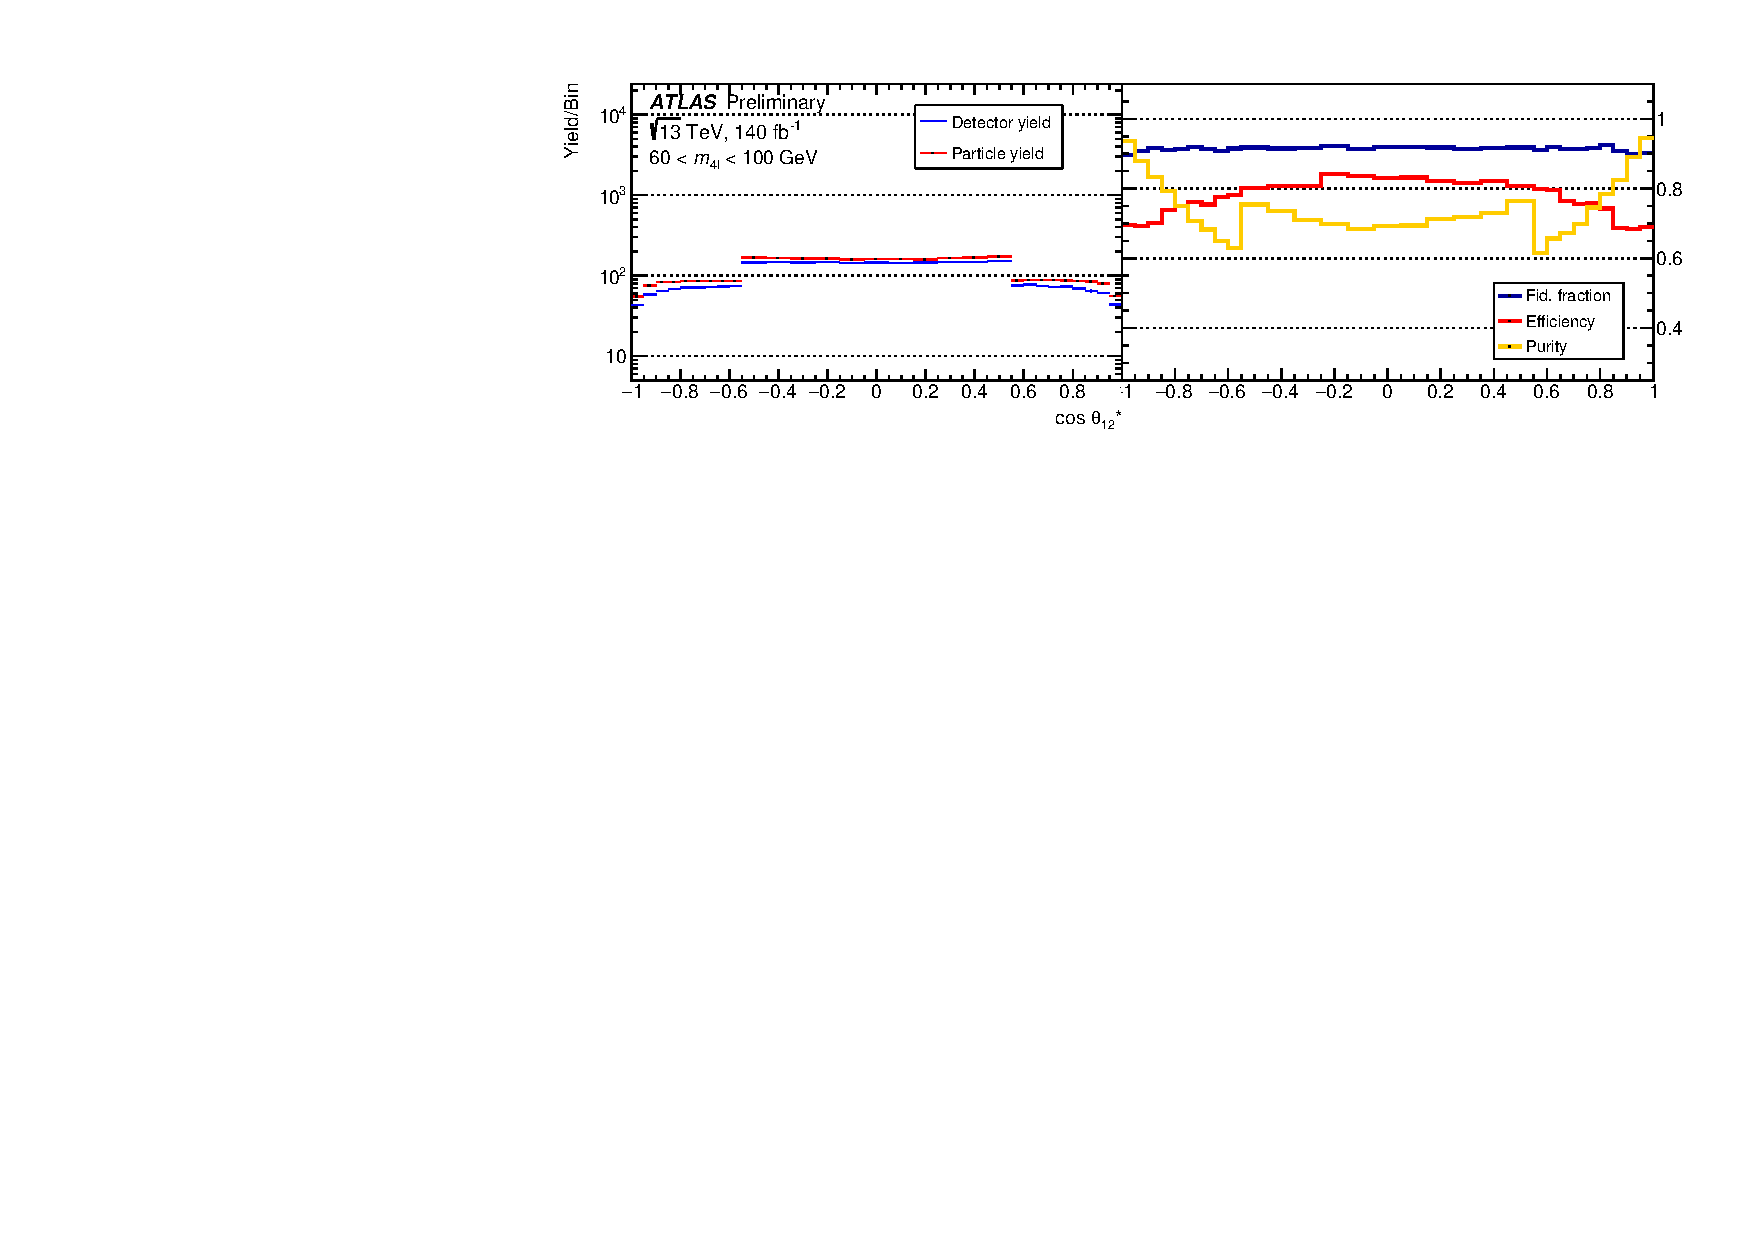
\includegraphics[width = 0.75\textwidth]{Figures/m4l/UnfoldingStudies/v014_inputs/cosThetaStar1_m4l60-100inputs.pdf}
    \end{subfigure}
    \begin{subfigure}{.99\textwidth}\centering
        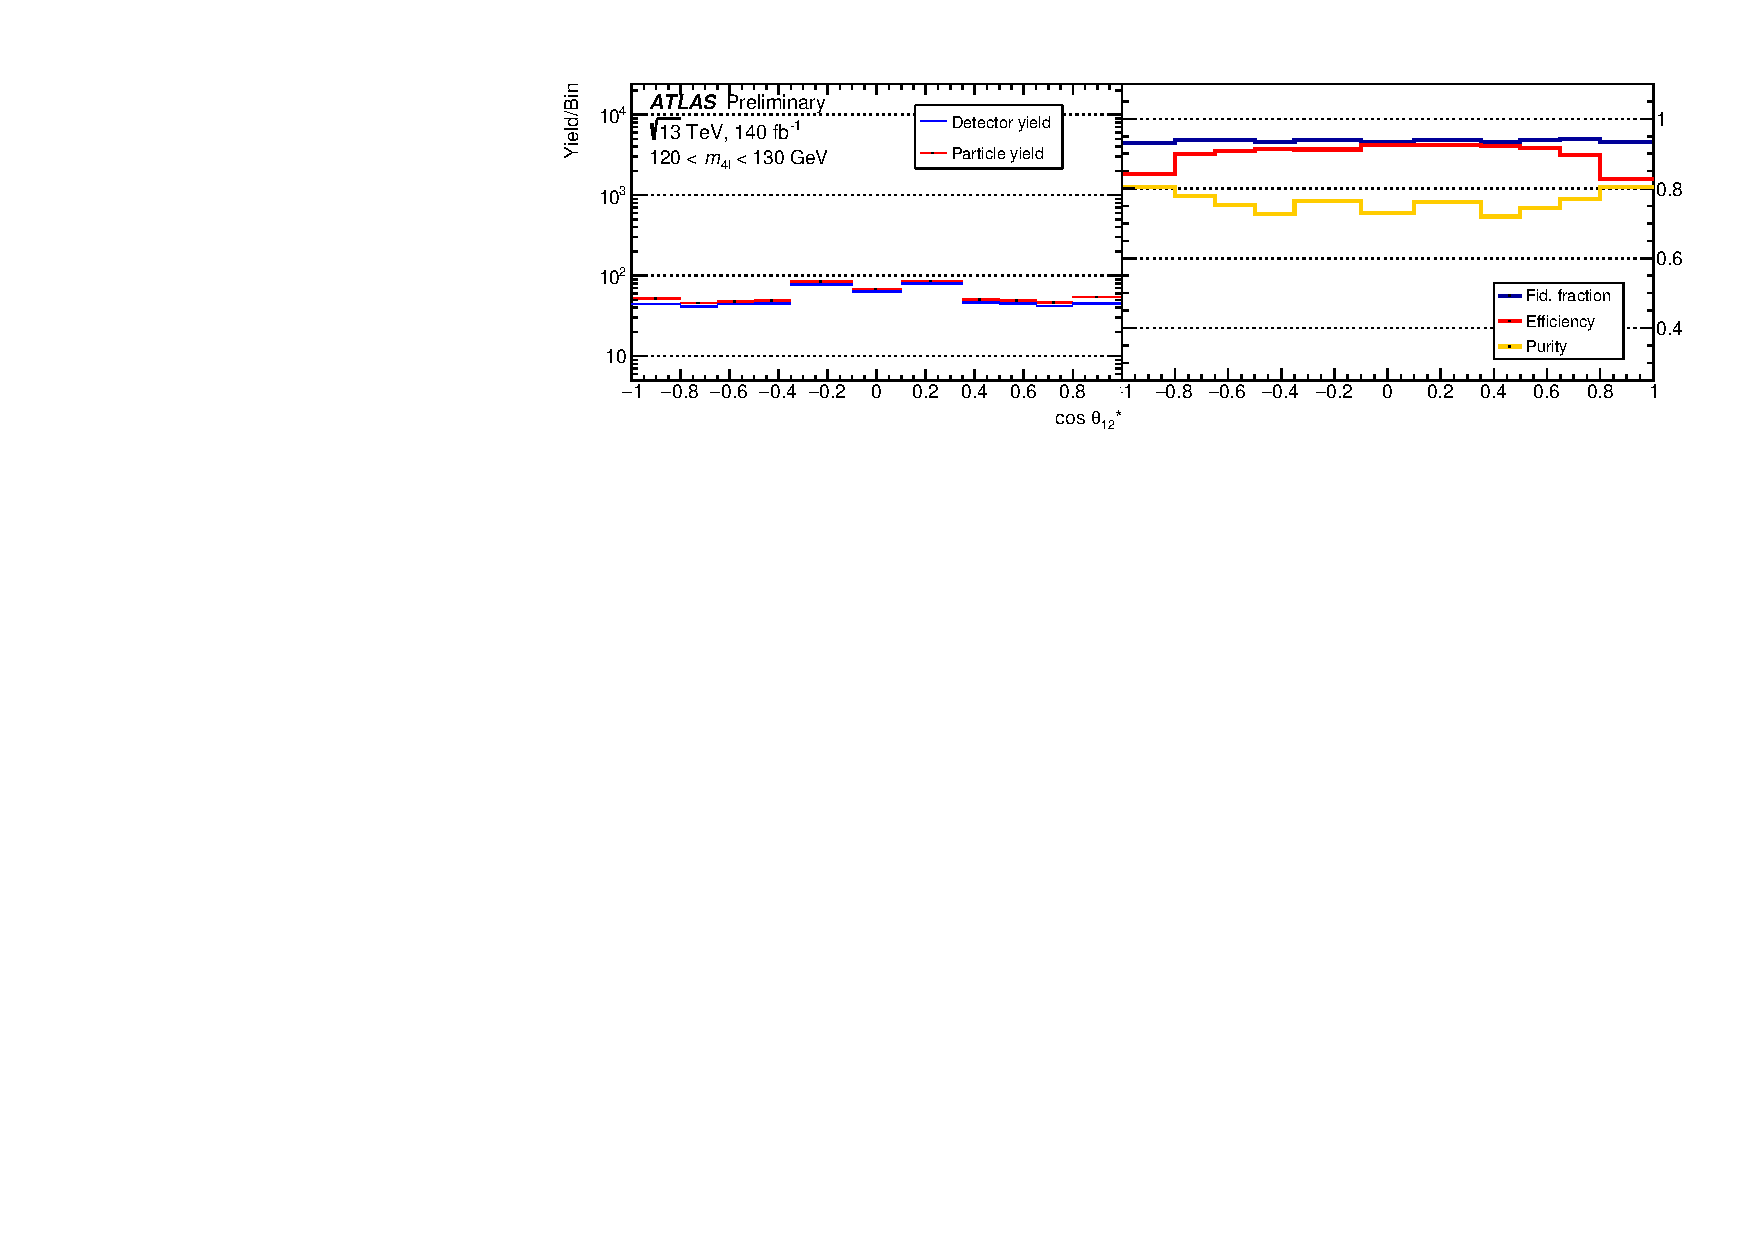
\includegraphics[width = 0.75\textwidth]{Figures/m4l/UnfoldingStudies/v014_inputs/cosThetaStar1_m4l120-130inputs.pdf}
    \end{subfigure}
    \begin{subfigure}{.99\textwidth}\centering
        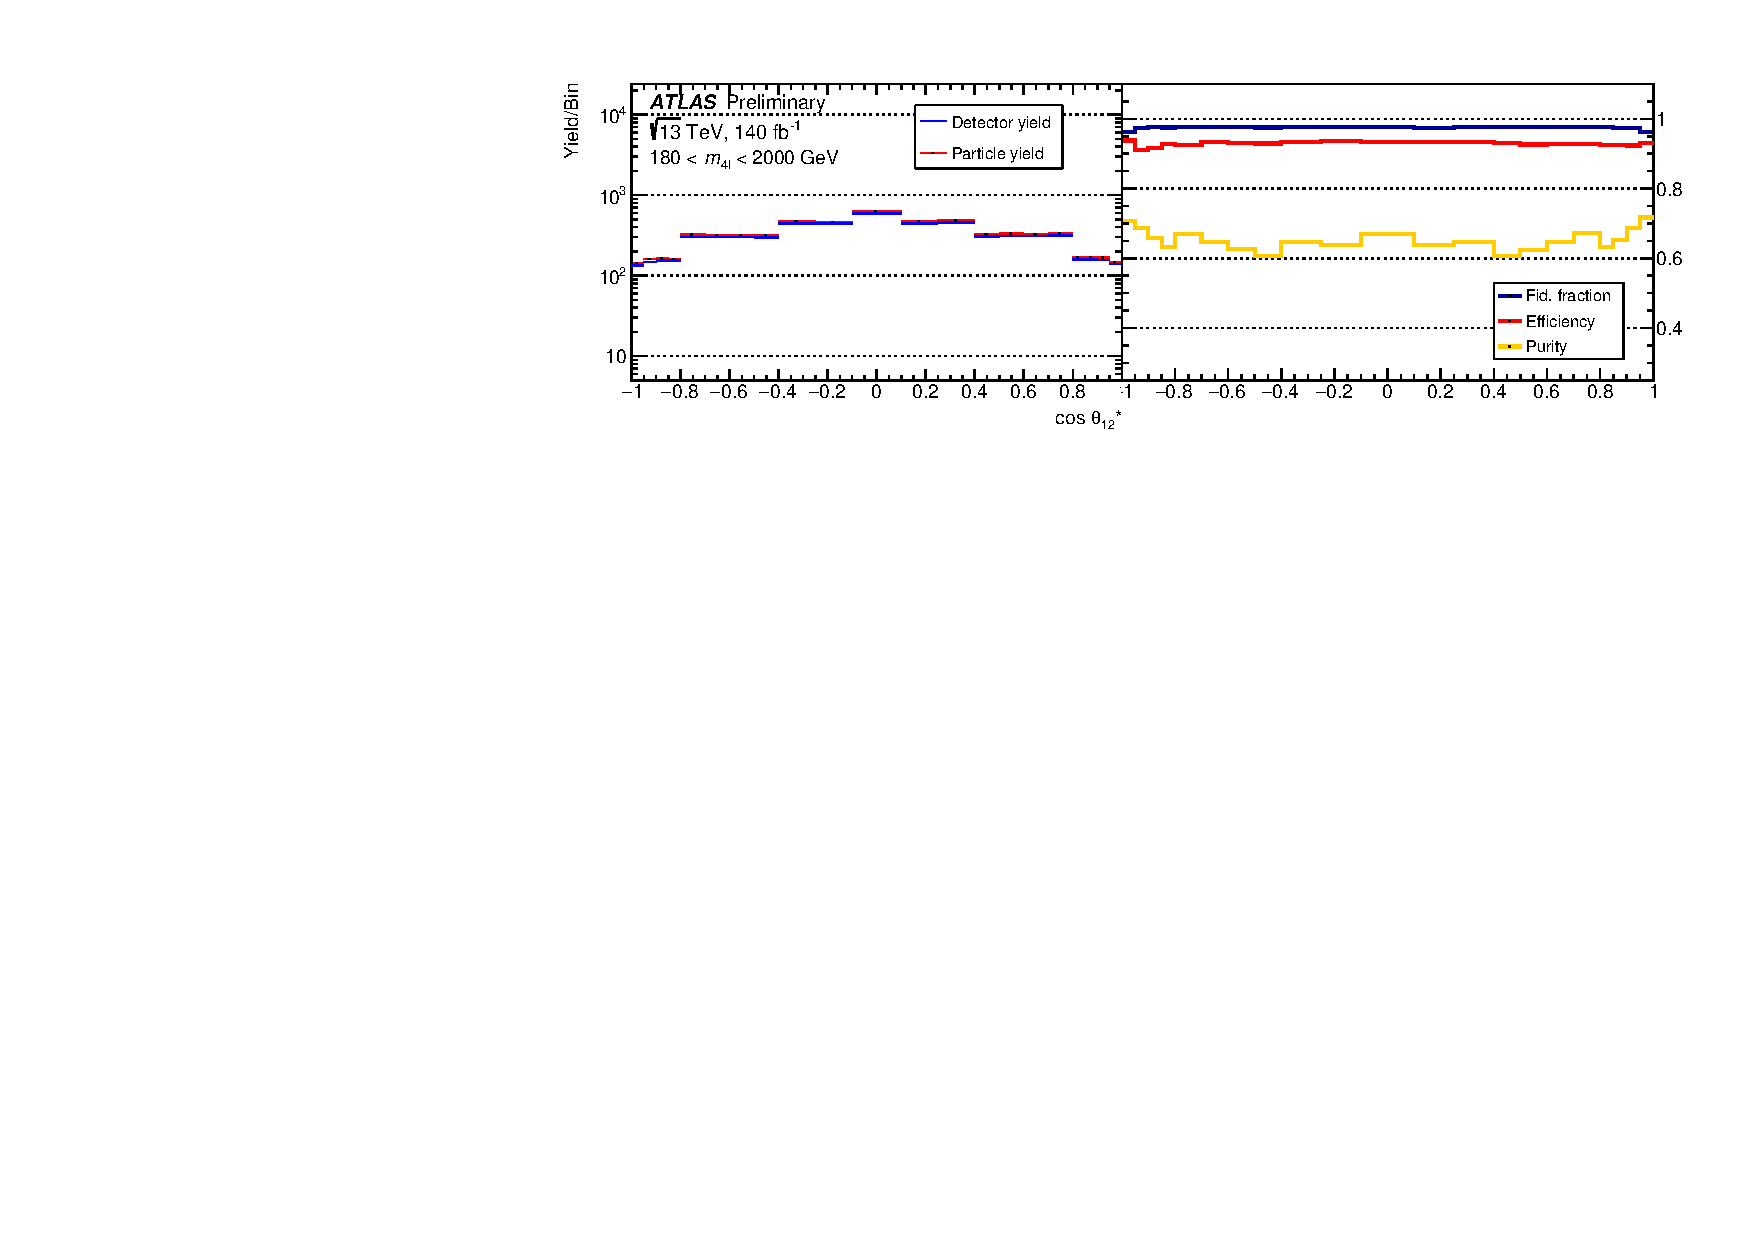
\includegraphics[width = 0.75\textwidth]{Figures/m4l/UnfoldingStudies/v014_inputs/cosThetaStar1_m4l180-2000inputs.pdf}
    \end{subfigure}
    \begin{subfigure}{.99\textwidth}\centering
        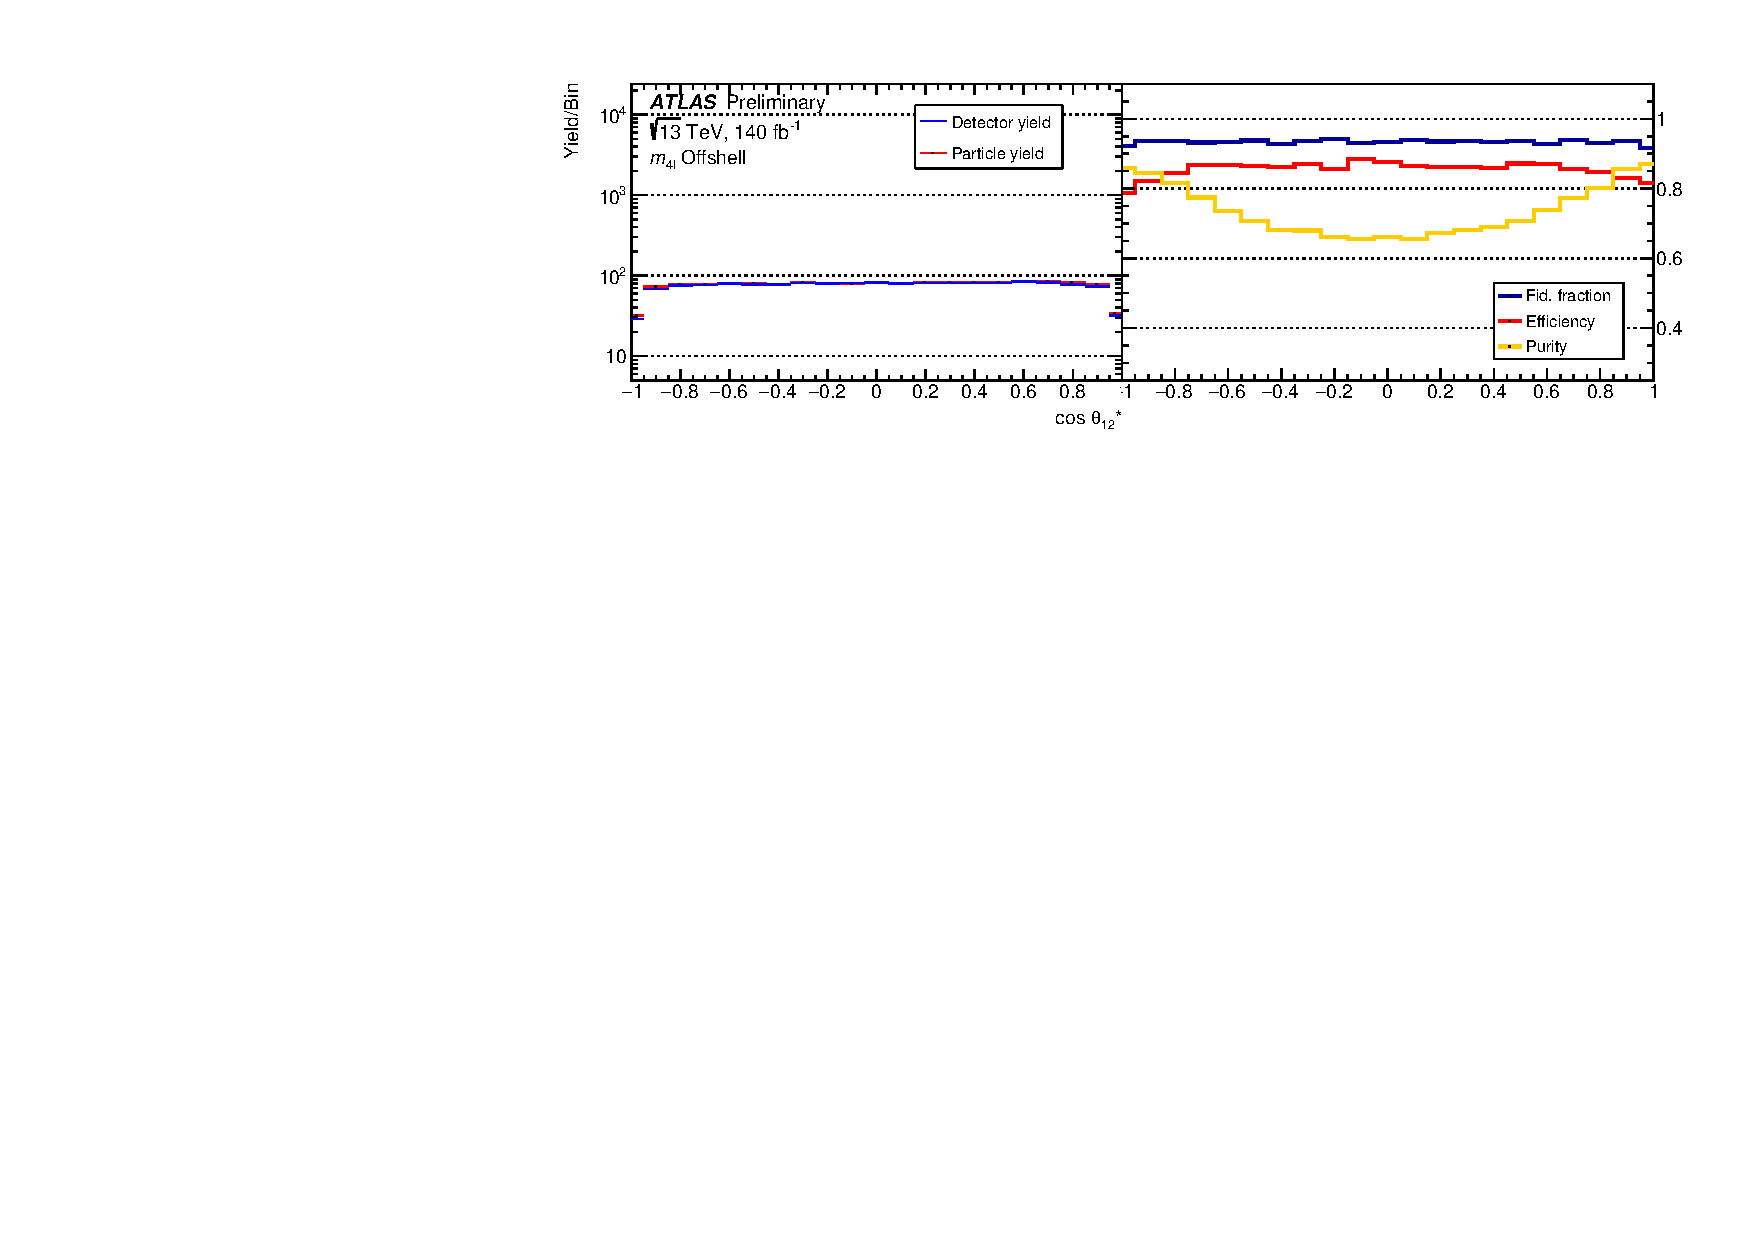
\includegraphics[width = 0.75\textwidth]{Figures/m4l/UnfoldingStudies/v014_inputs/cosThetaStar1_m4loffshellinputs.pdf}
    \end{subfigure}
    \caption{In the left-hand panels, the number of predicted events passing the reconstruction- and fiducial- level selections are displayed as the detector yield and particle yield, respectively. The right-hand panel shows the efficiency, fiducial purity and fiducial fraction. All variables are plotted as a function of the \costhetastar bins, in slices of the \mFourL variable which are stacked and labelled with the included \mFourL range.
    \label{fig:costhet1unf}}
\end{figure}  

\FloatBarrier
\clearpage

\begin{figure}[htb]
    \centering 
    \begin{subfigure}{.99\textwidth}\centering
        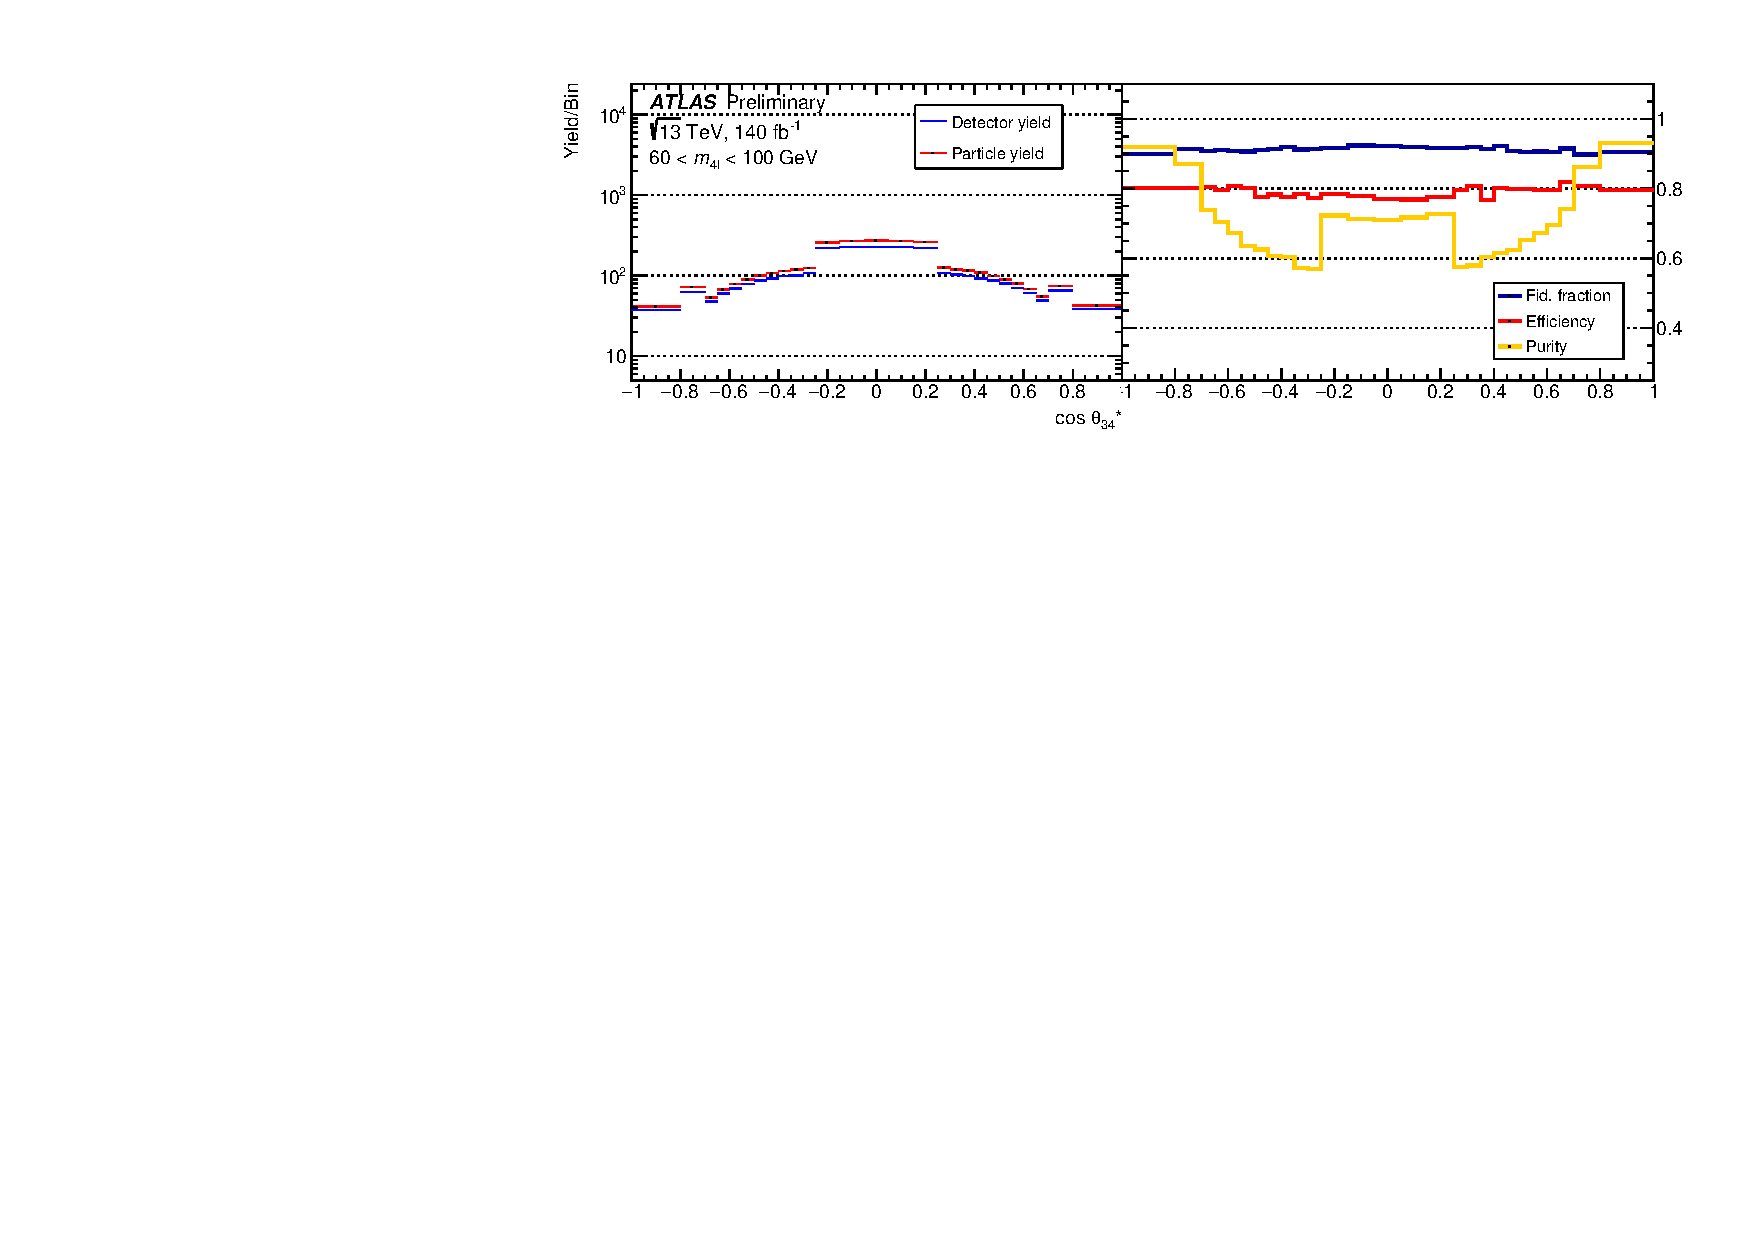
\includegraphics[width = 0.75\textwidth]{Figures/m4l/UnfoldingStudies/v014_inputs/cosThetaStar3_m4l60-100inputs.pdf}
    \end{subfigure}
    \begin{subfigure}{.99\textwidth}\centering
        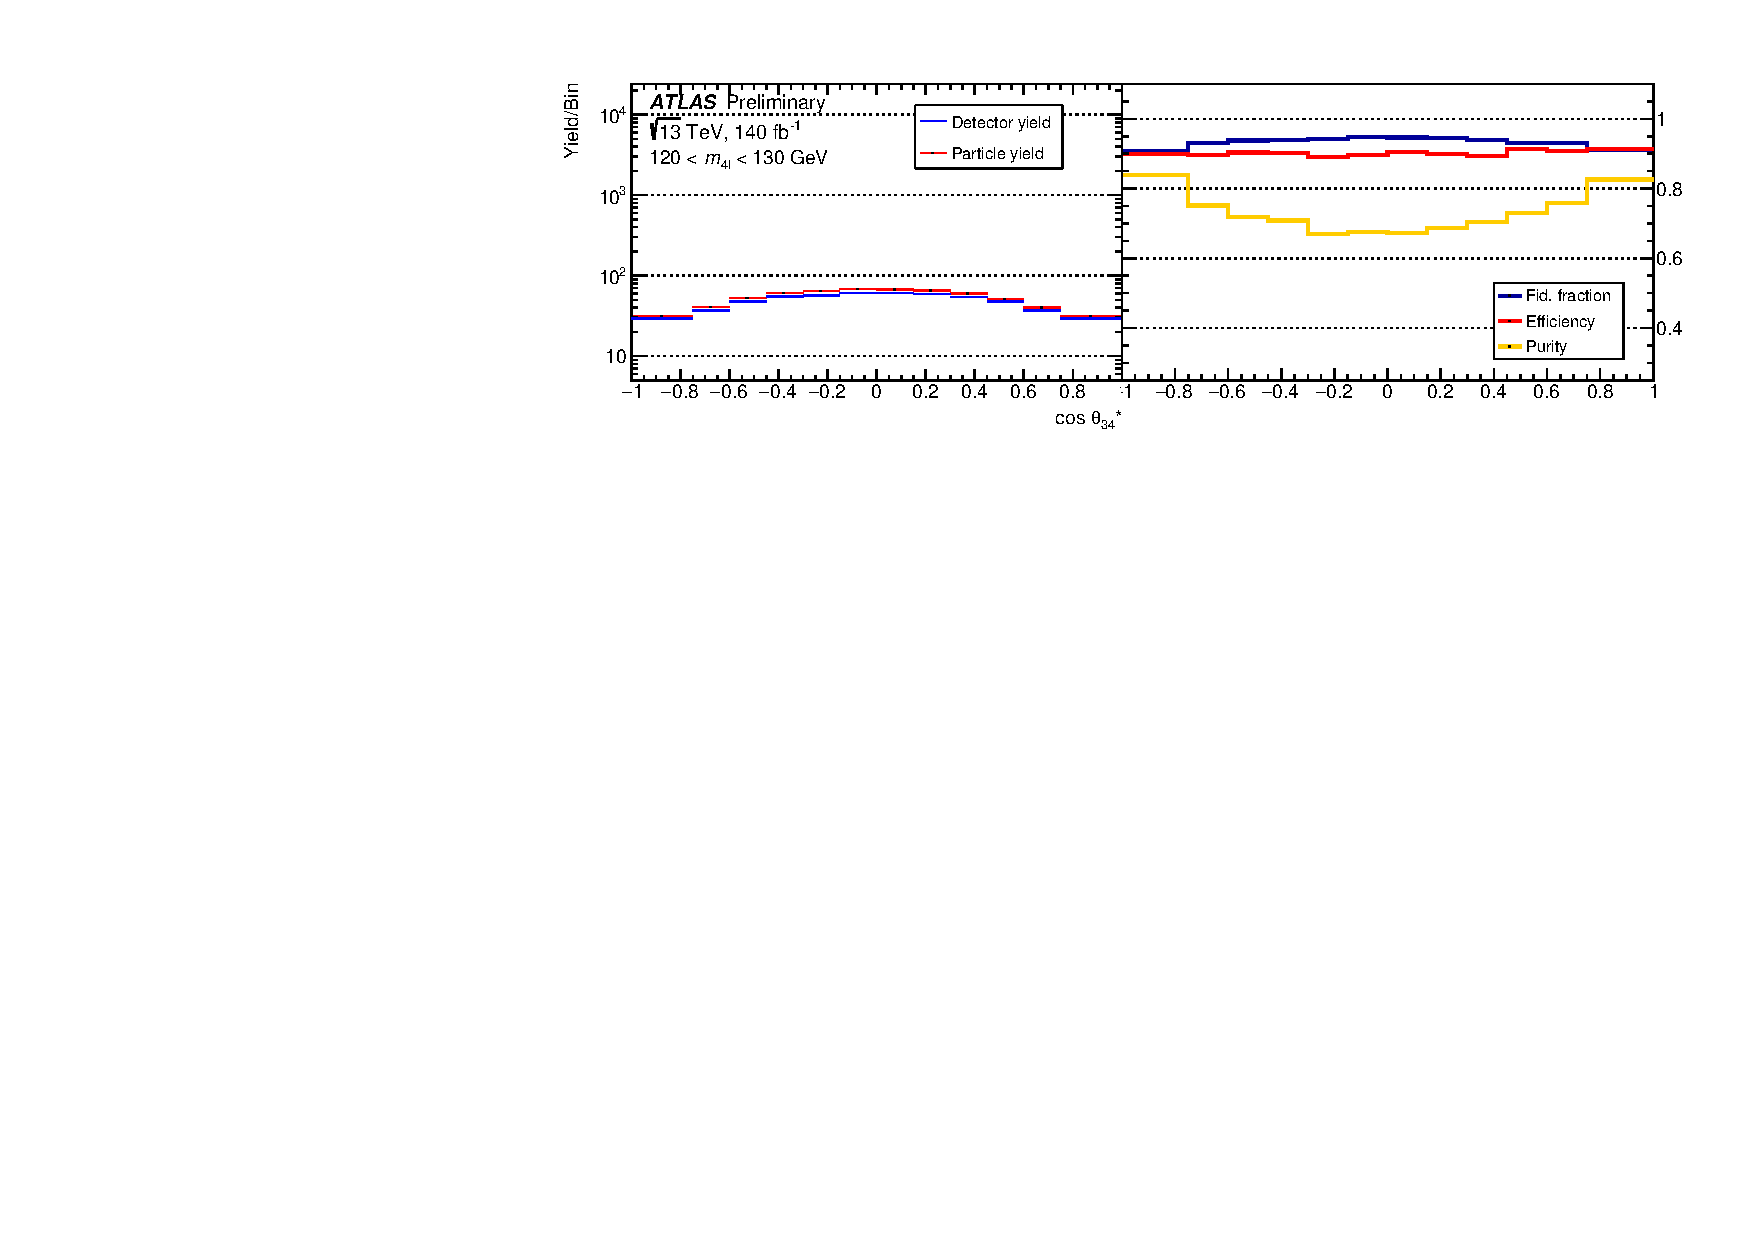
\includegraphics[width = 0.75\textwidth]{Figures/m4l/UnfoldingStudies/v014_inputs/cosThetaStar3_m4l120-130inputs.pdf}
    \end{subfigure}
    \begin{subfigure}{.99\textwidth}\centering
        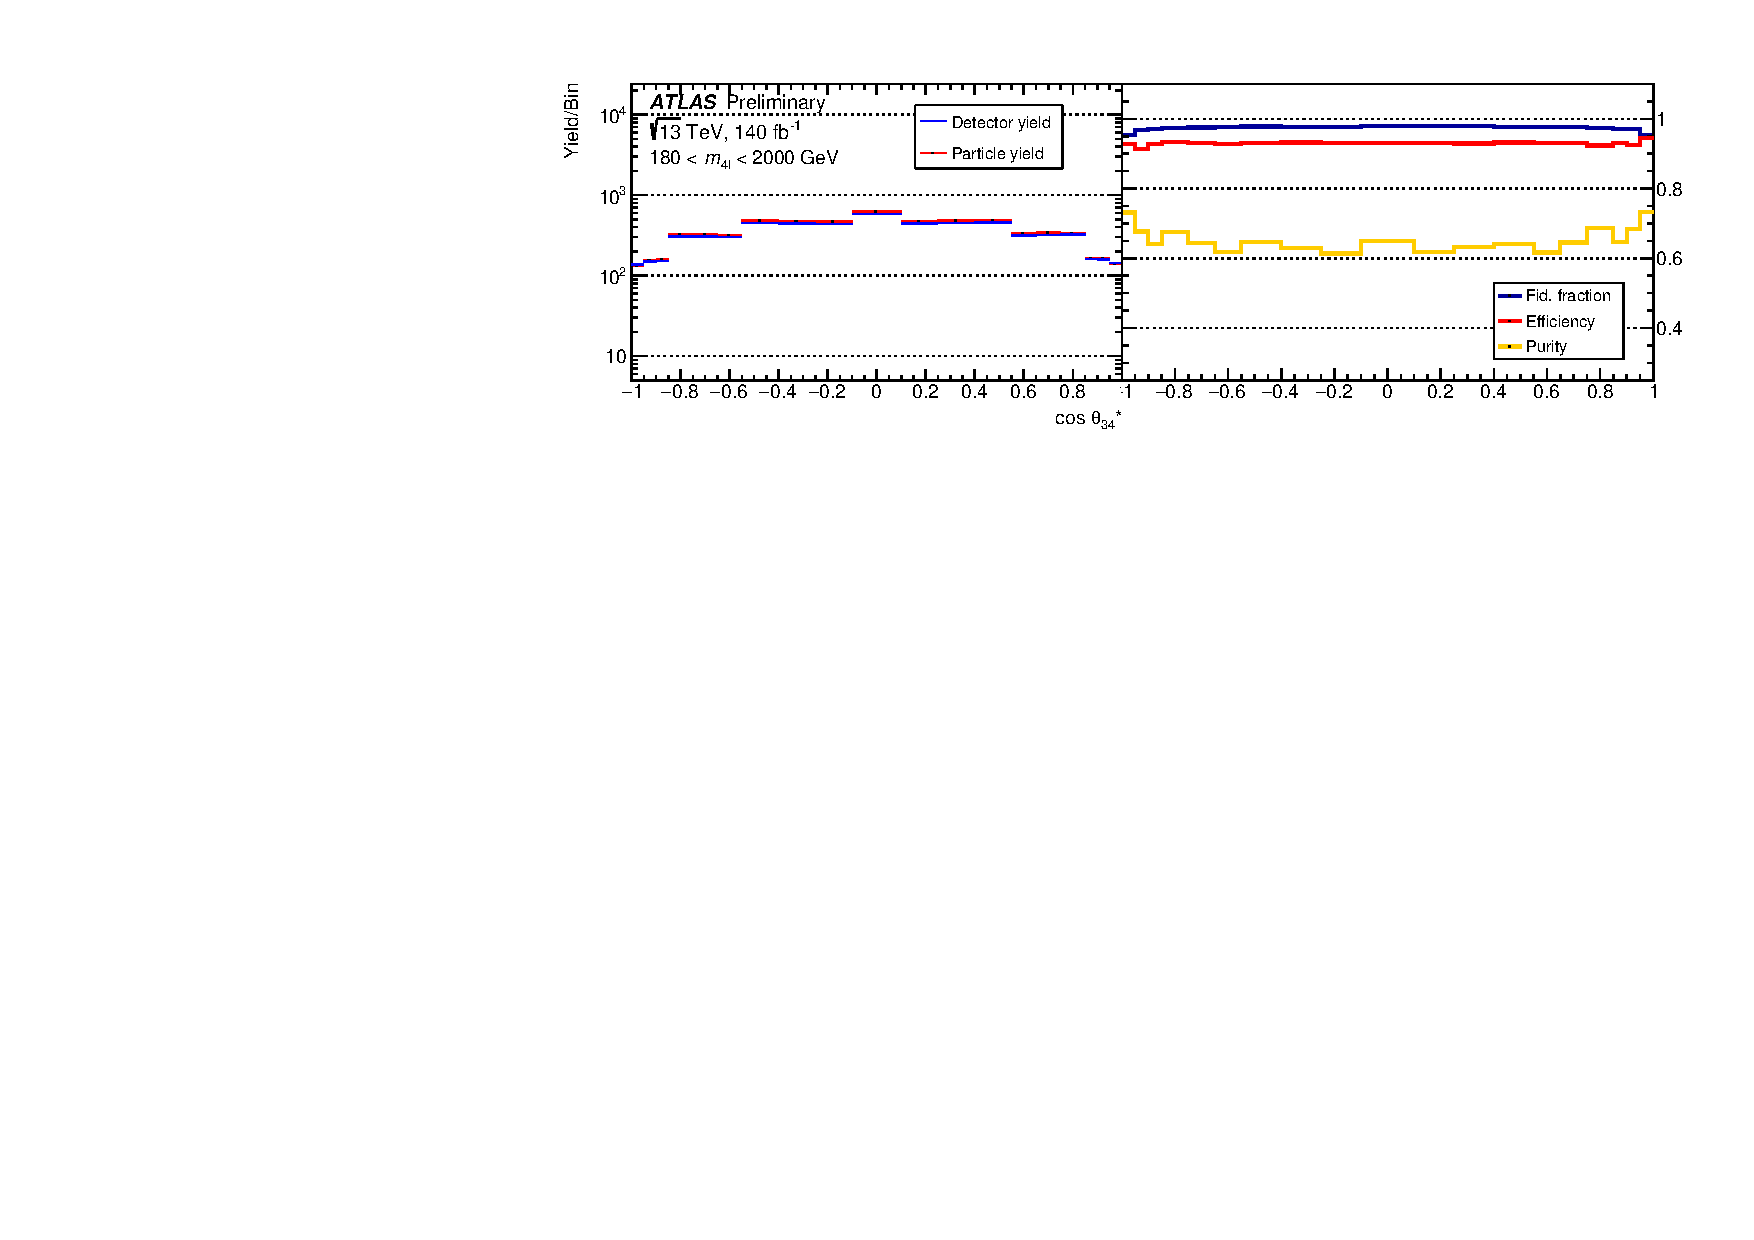
\includegraphics[width = 0.75\textwidth]{Figures/m4l/UnfoldingStudies/v014_inputs/cosThetaStar3_m4l180-2000inputs.pdf}
    \end{subfigure}
    \begin{subfigure}{.99\textwidth}\centering
        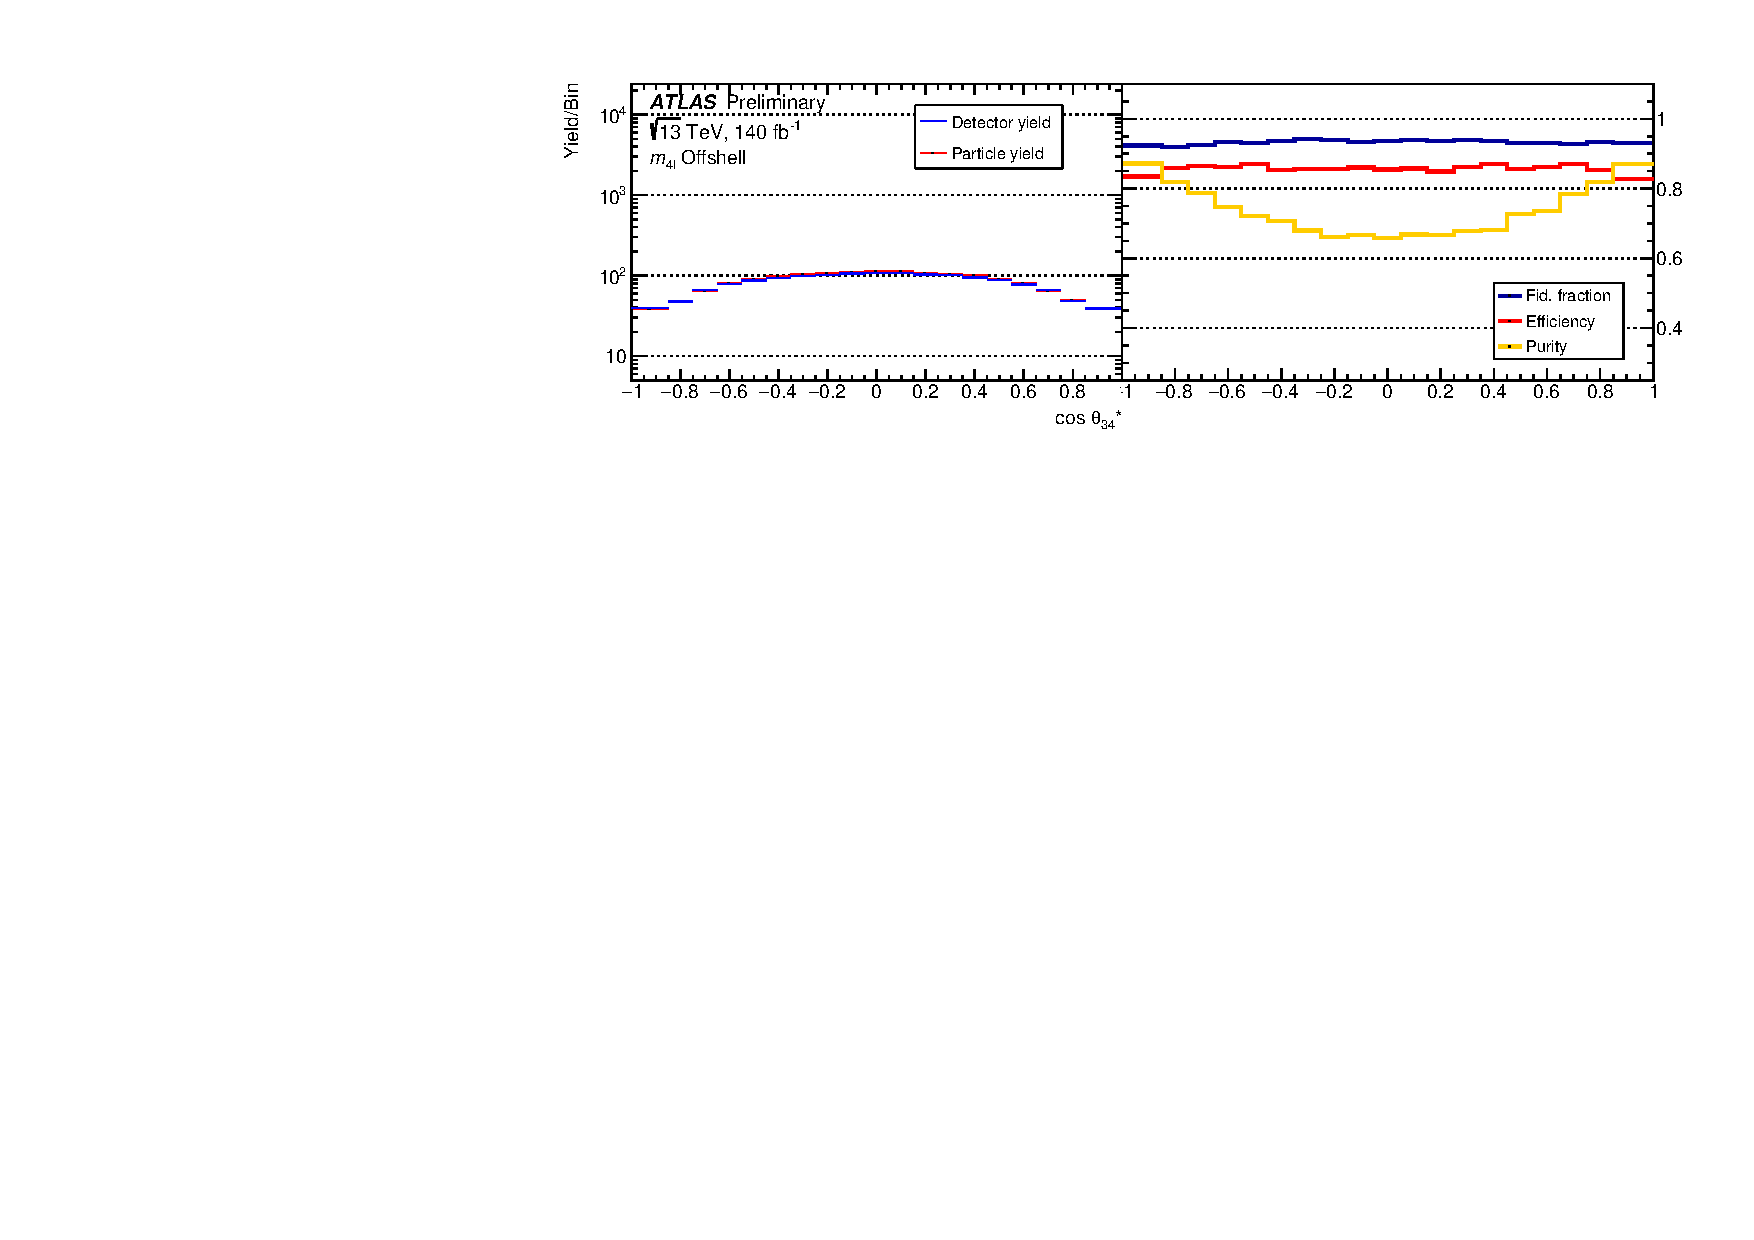
\includegraphics[width = 0.75\textwidth]{Figures/m4l/UnfoldingStudies/v014_inputs/cosThetaStar3_m4loffshellinputs.pdf}
    \end{subfigure}
    \caption{In the left-hand panels, the number of predicted events passing the reconstruction- and fiducial- level selections are displayed as the detector yield and particle yield, respectively. The right-hand panel shows the efficiency, fiducial purity and fiducial fraction. All variables are plotted as a function of the \costhetastar bins, in slices of the \mFourL variable which are stacked and labelled with the included \mFourL range.
    \label{fig:costhet2unf}}
\end{figure}  

\FloatBarrier
\clearpage

\begin{figure}[htb]
    \centering 
    \begin{subfigure}{.99\textwidth}\centering
        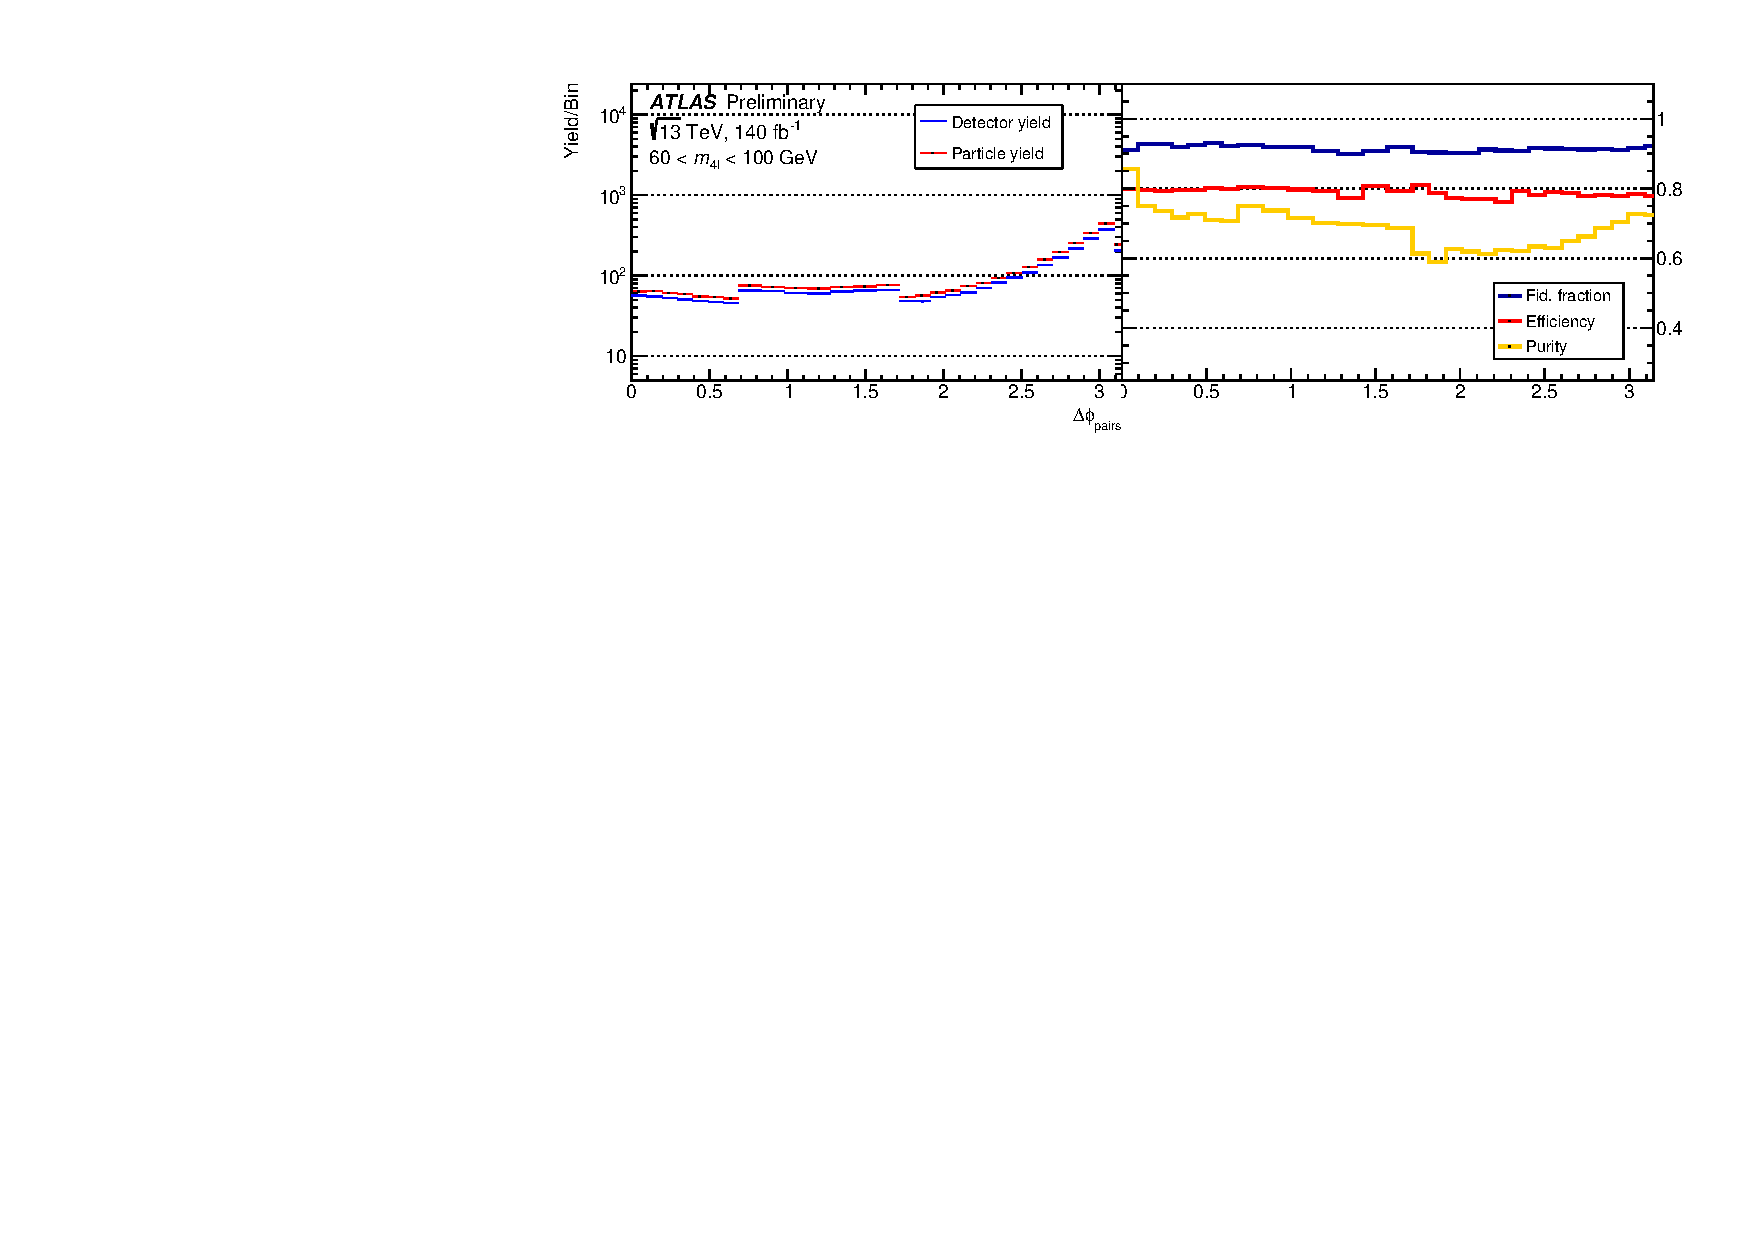
\includegraphics[width = 0.75\textwidth]{Figures/m4l/UnfoldingStudies/v014_inputs/deltaPhiPairs_m4l60-100inputs.pdf}
    \end{subfigure}
    \begin{subfigure}{.99\textwidth}\centering
        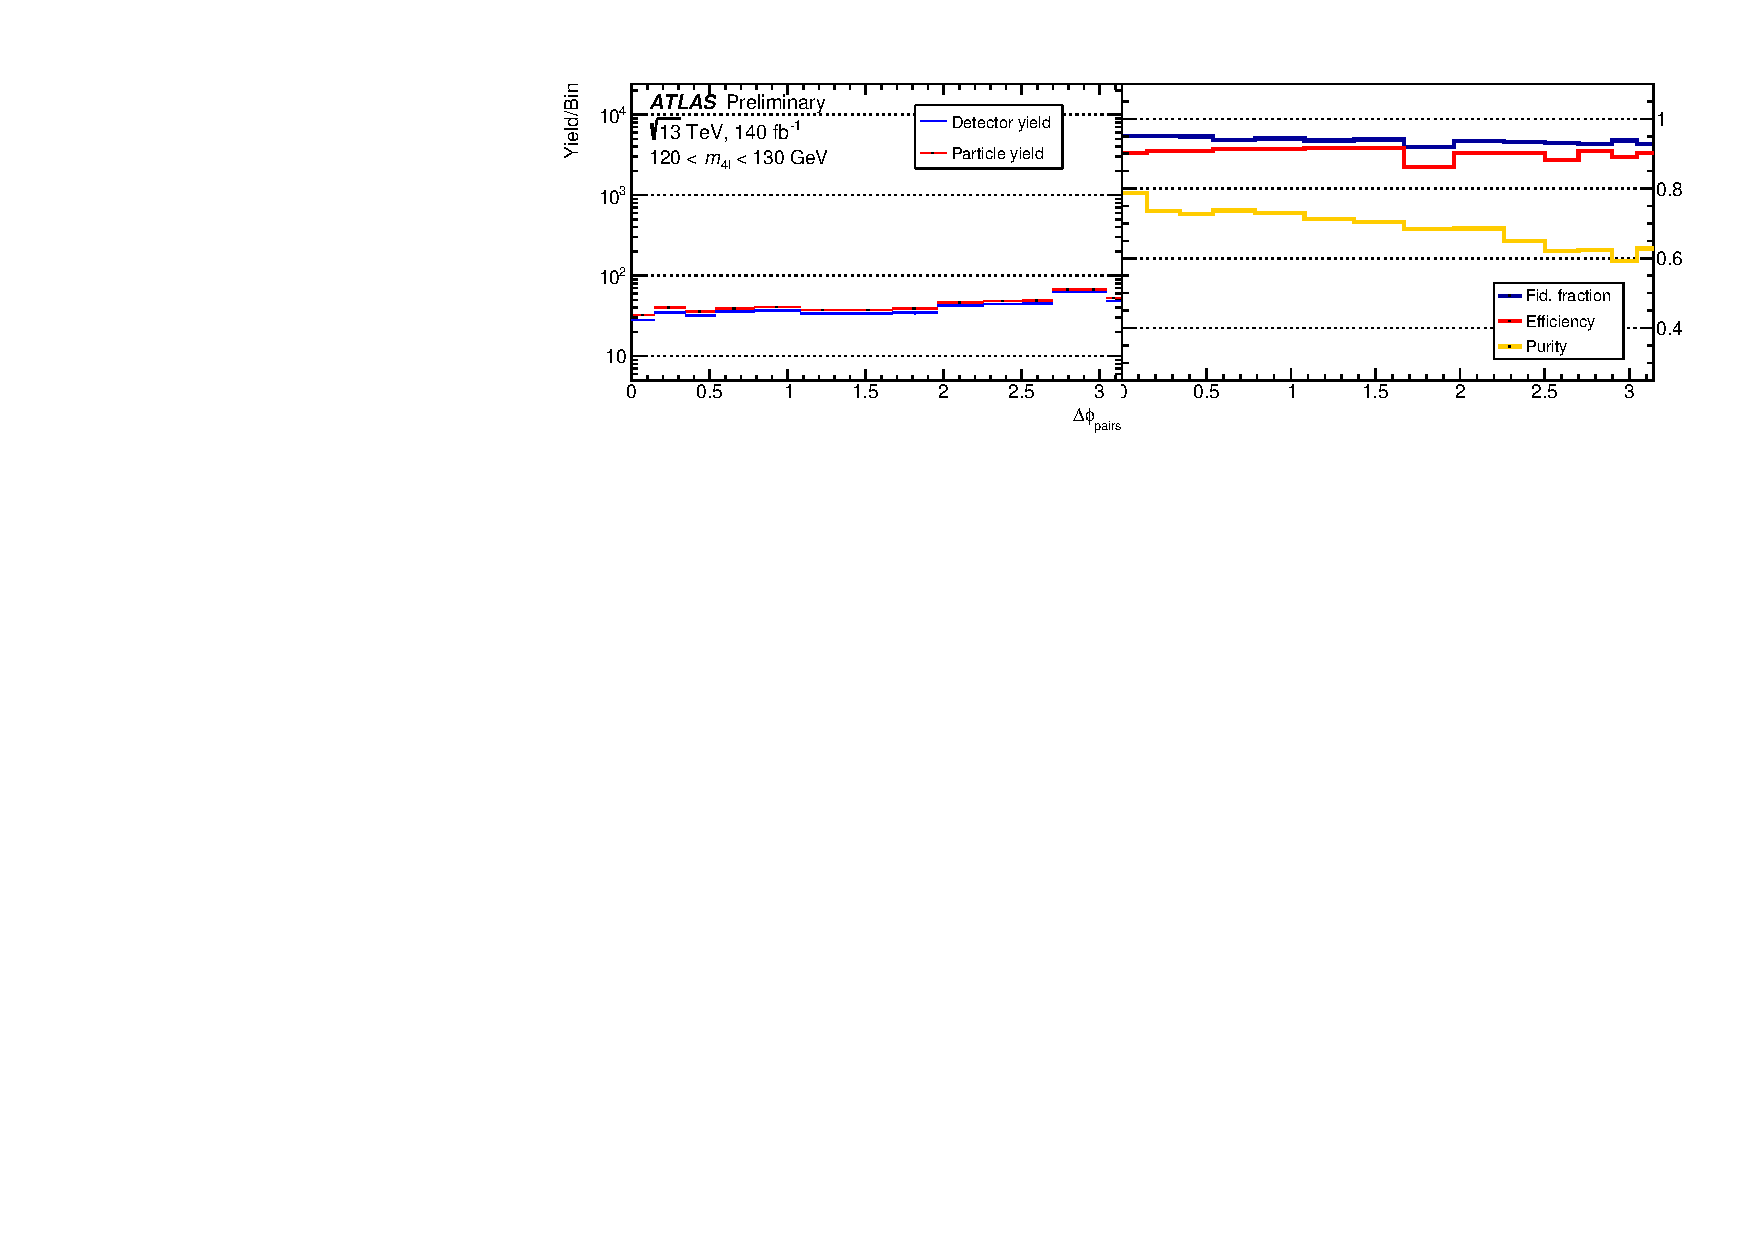
\includegraphics[width = 0.75\textwidth]{Figures/m4l/UnfoldingStudies/v014_inputs/deltaPhiPairs_m4l120-130inputs.pdf}
    \end{subfigure}
    \begin{subfigure}{.99\textwidth}\centering
        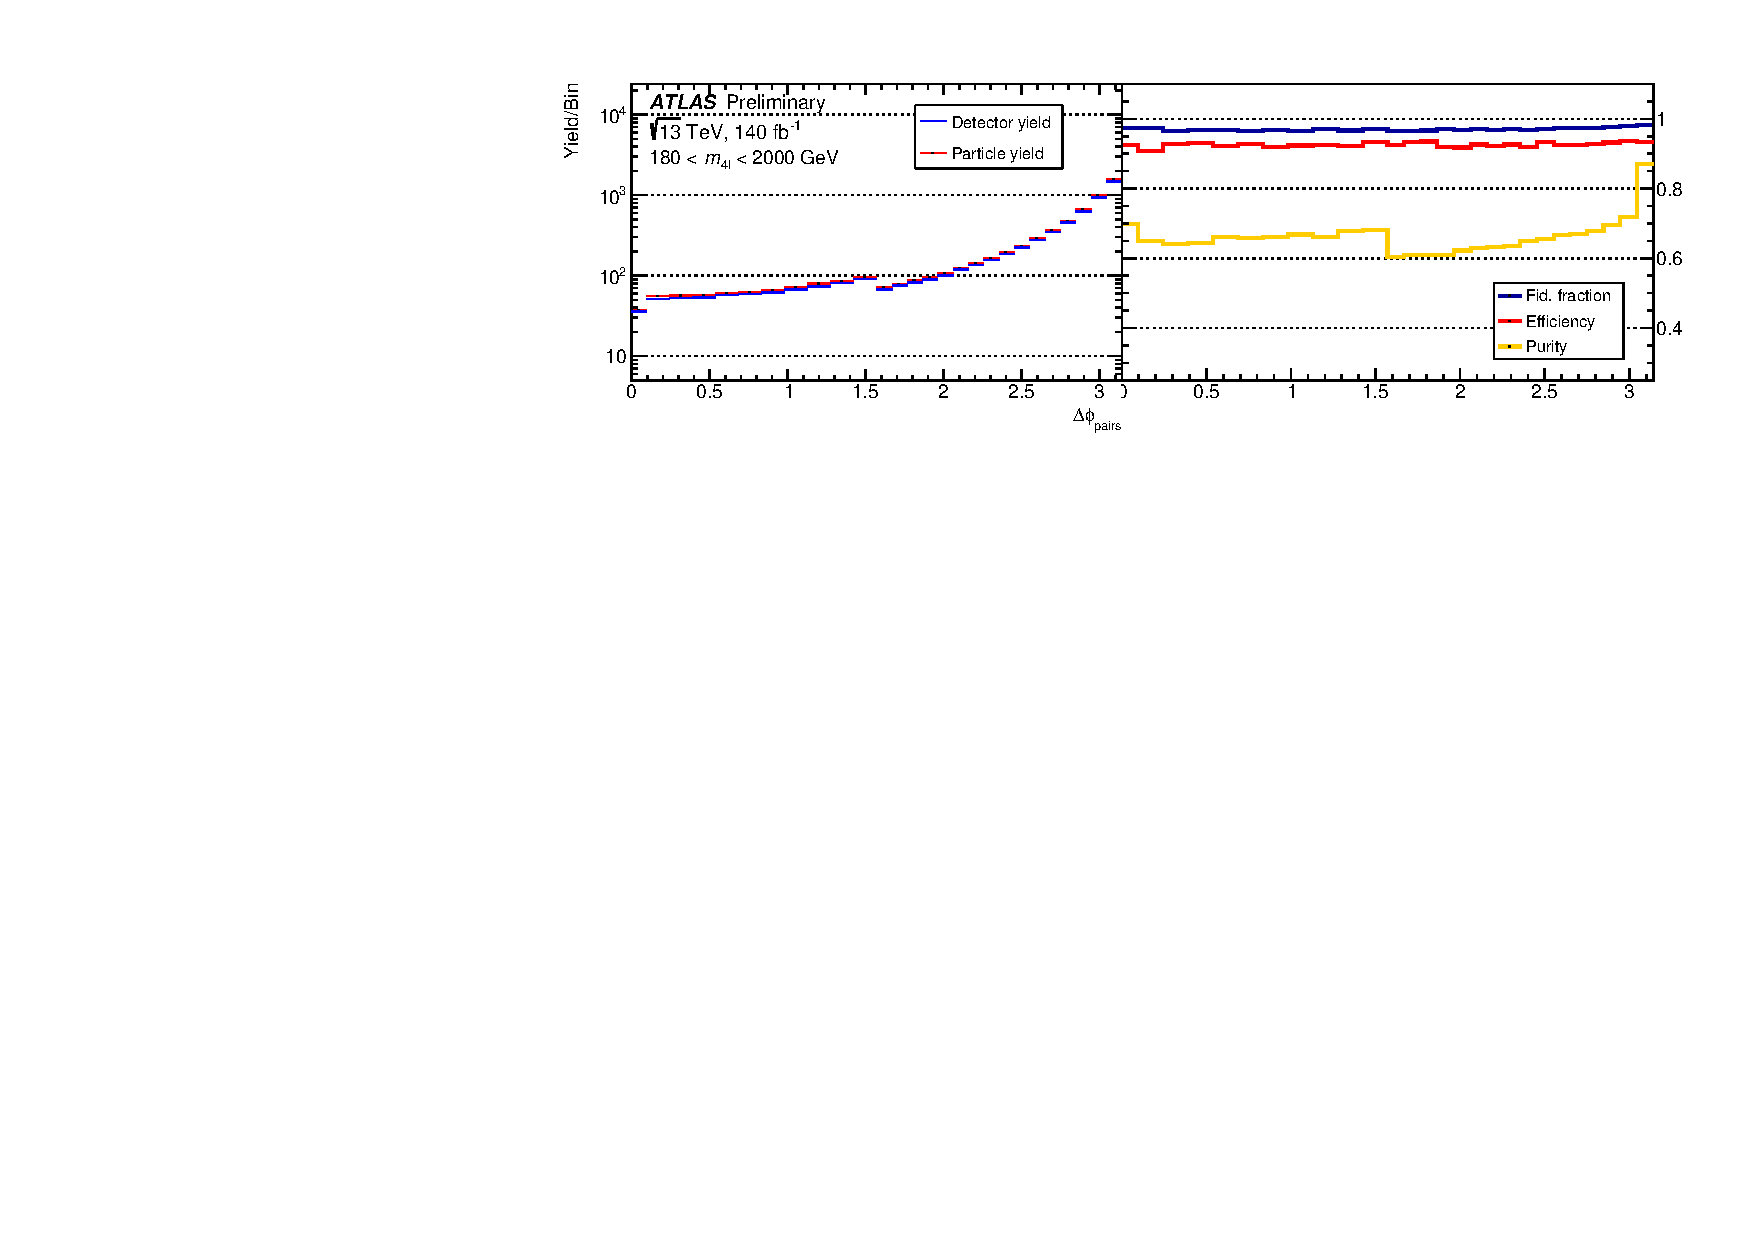
\includegraphics[width = 0.75\textwidth]{Figures/m4l/UnfoldingStudies/v014_inputs/deltaPhiPairs_m4l180-2000inputs.pdf}
    \end{subfigure}
    \begin{subfigure}{.99\textwidth}\centering
        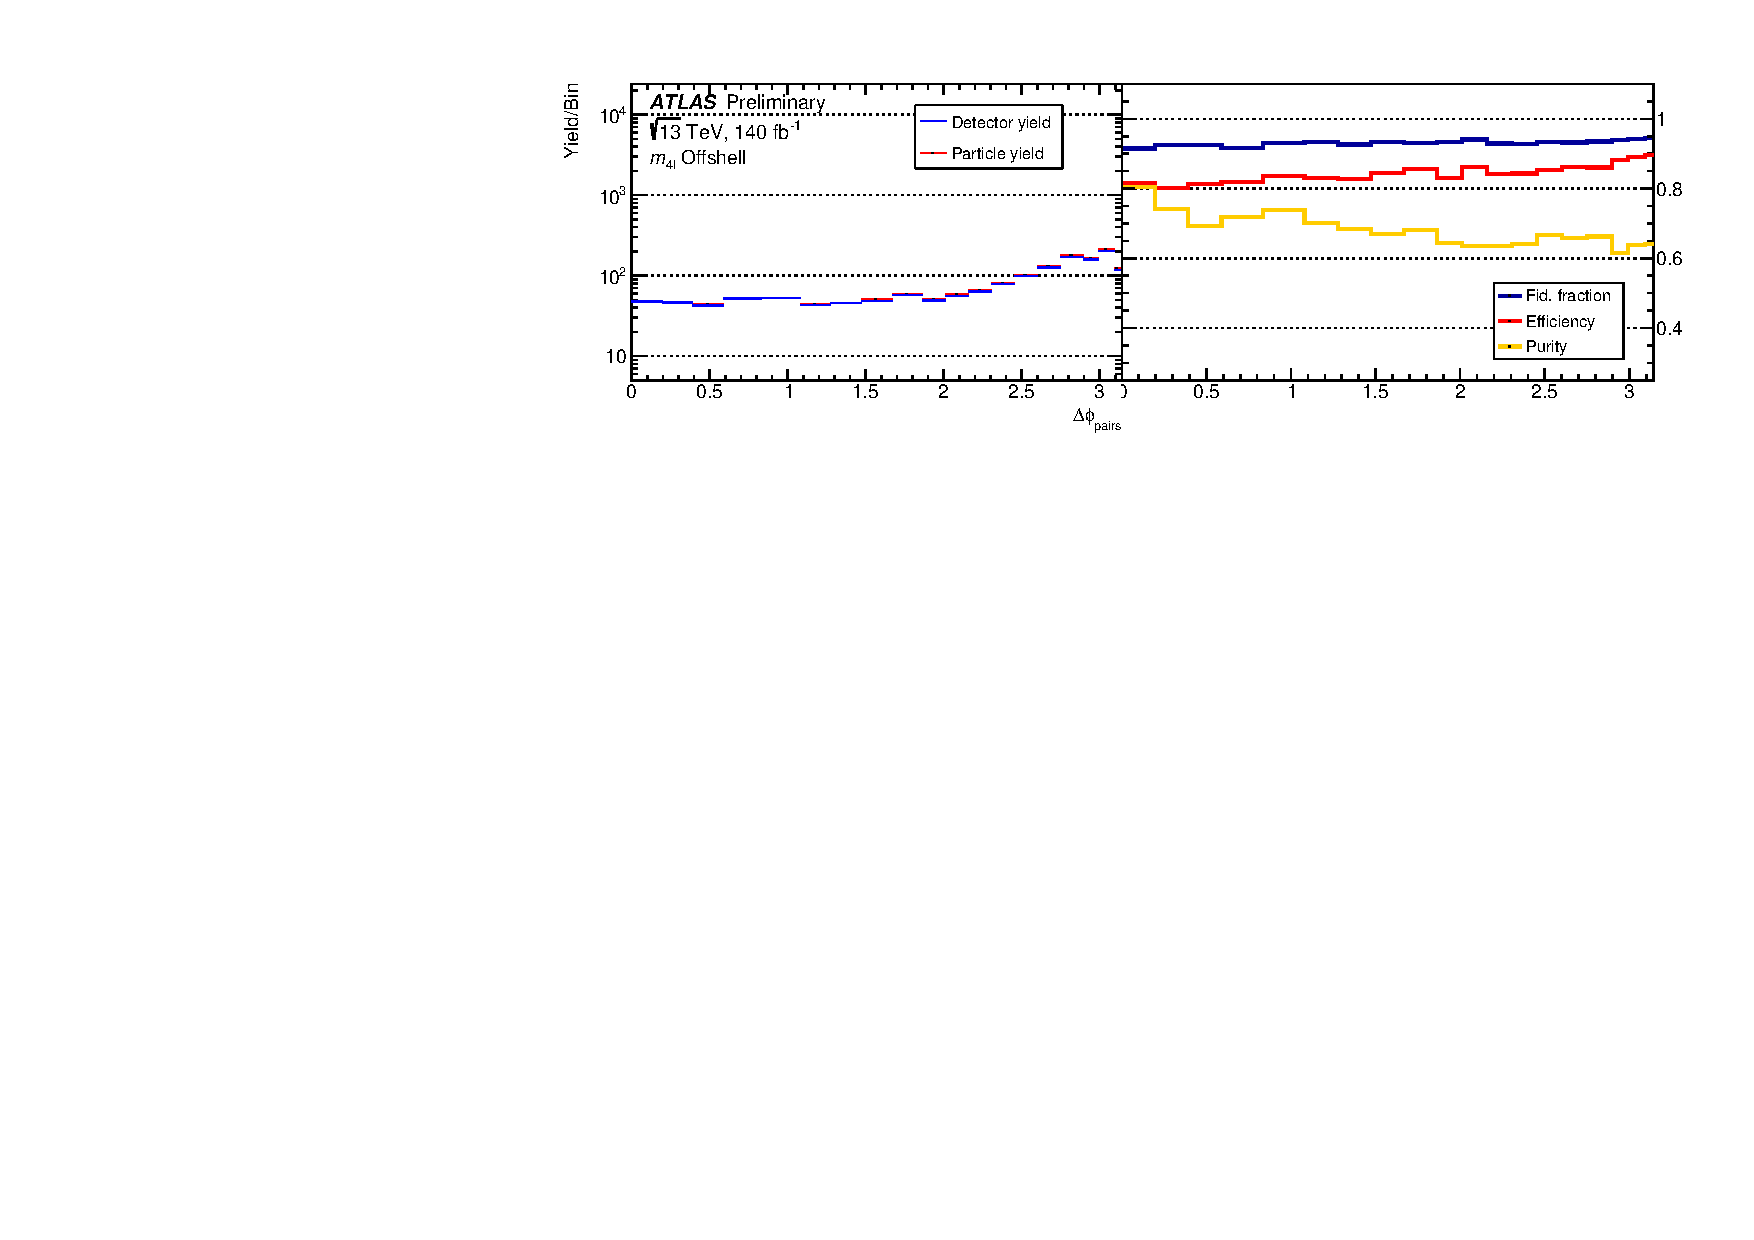
\includegraphics[width = 0.75\textwidth]{Figures/m4l/UnfoldingStudies/v014_inputs/deltaPhiPairs_m4loffshellinputs.pdf}
    \end{subfigure}
    \caption{In the left-hand panels, the number of predicted events passing the reconstruction- and fiducial- level selections are displayed as the detector yield and particle yield, respectively. The right-hand panel shows the efficiency, fiducial purity and fiducial fraction. All variables are plotted as a function of the \dPhiPairs bins, in slices of the \mFourL variable which are stacked and labelled with the included \mFourL range.
    \label{fig:dphipunf}}
\end{figure}  

\FloatBarrier
\clearpage

\begin{figure}[htb]
    \centering 
    \begin{subfigure}{.99\textwidth}\centering
        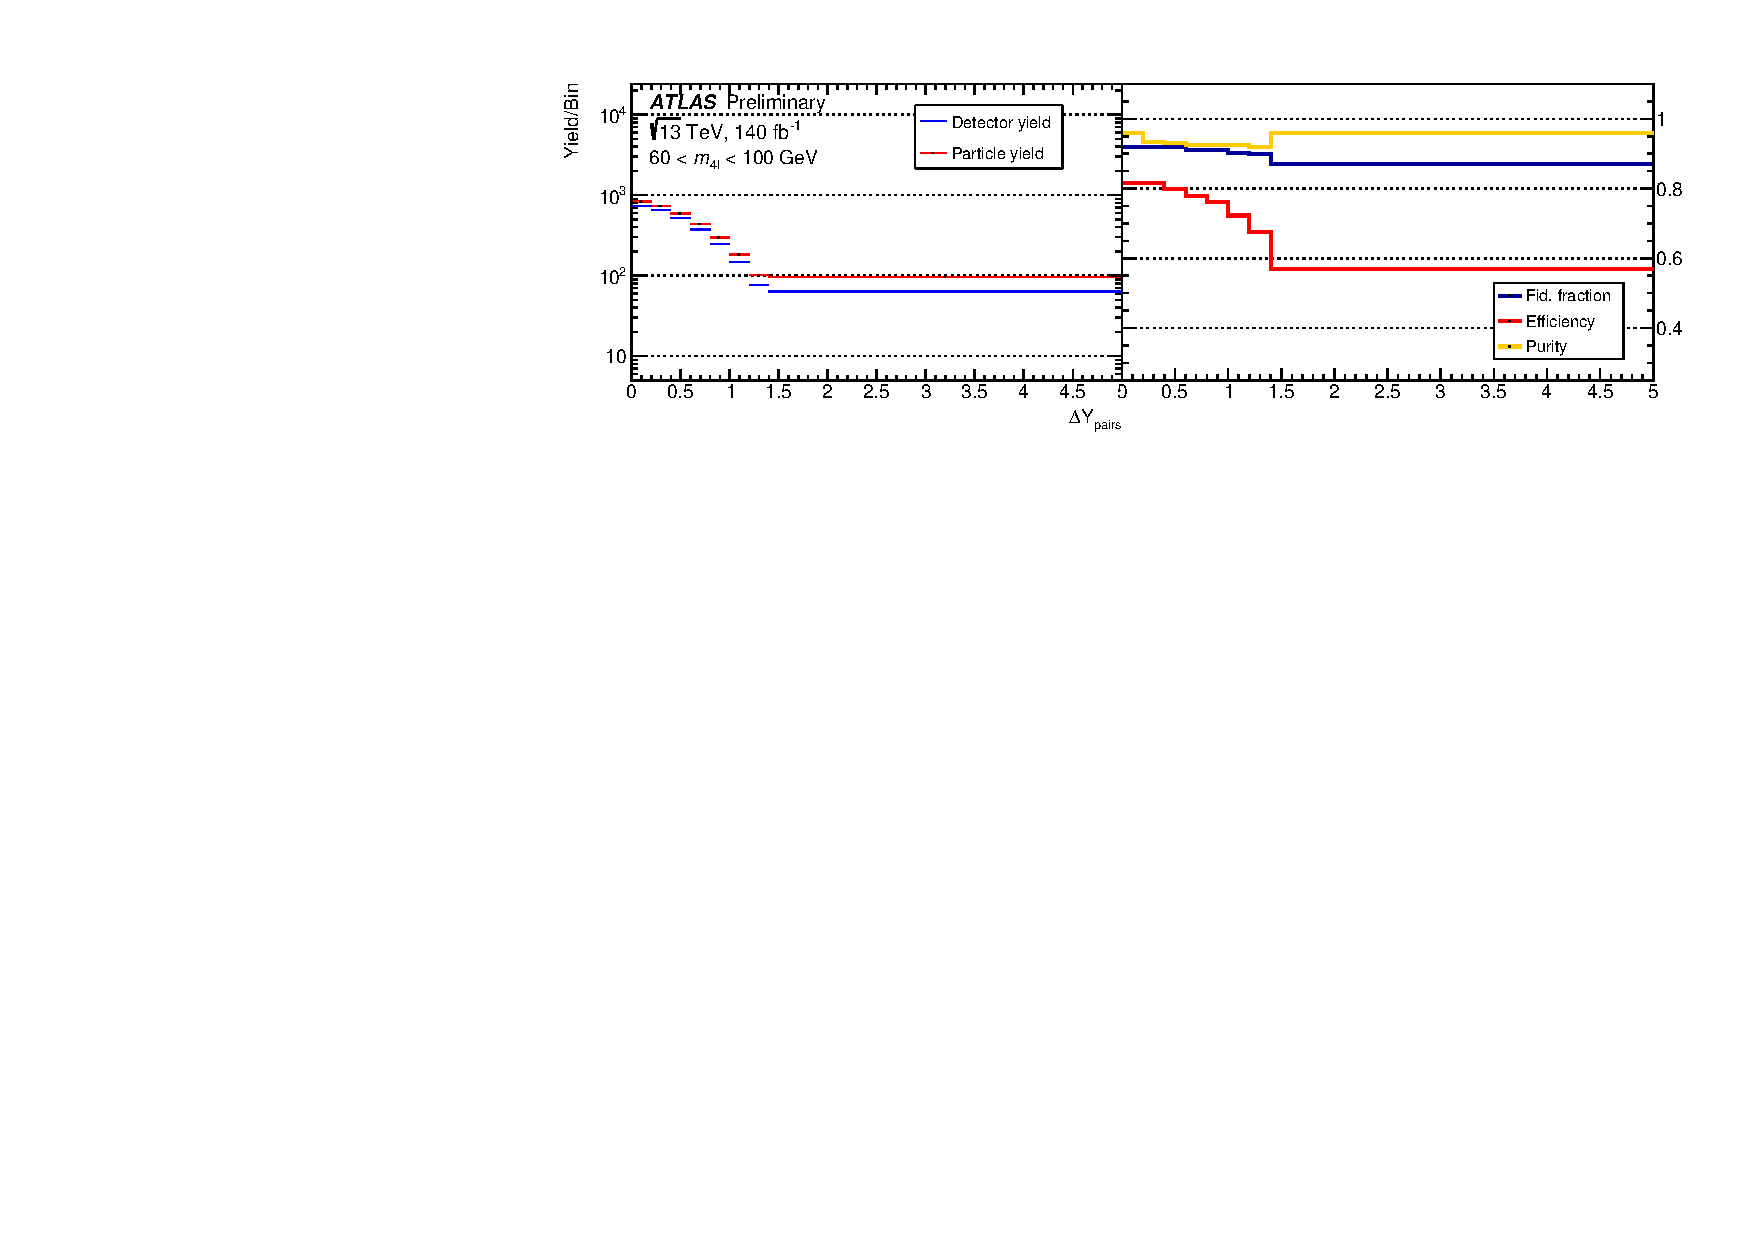
\includegraphics[width = 0.75\textwidth]{Figures/m4l/UnfoldingStudies/v014_inputs/deltaYPairs_m4l60-100inputs.pdf}
    \end{subfigure}
    \begin{subfigure}{.99\textwidth}\centering
        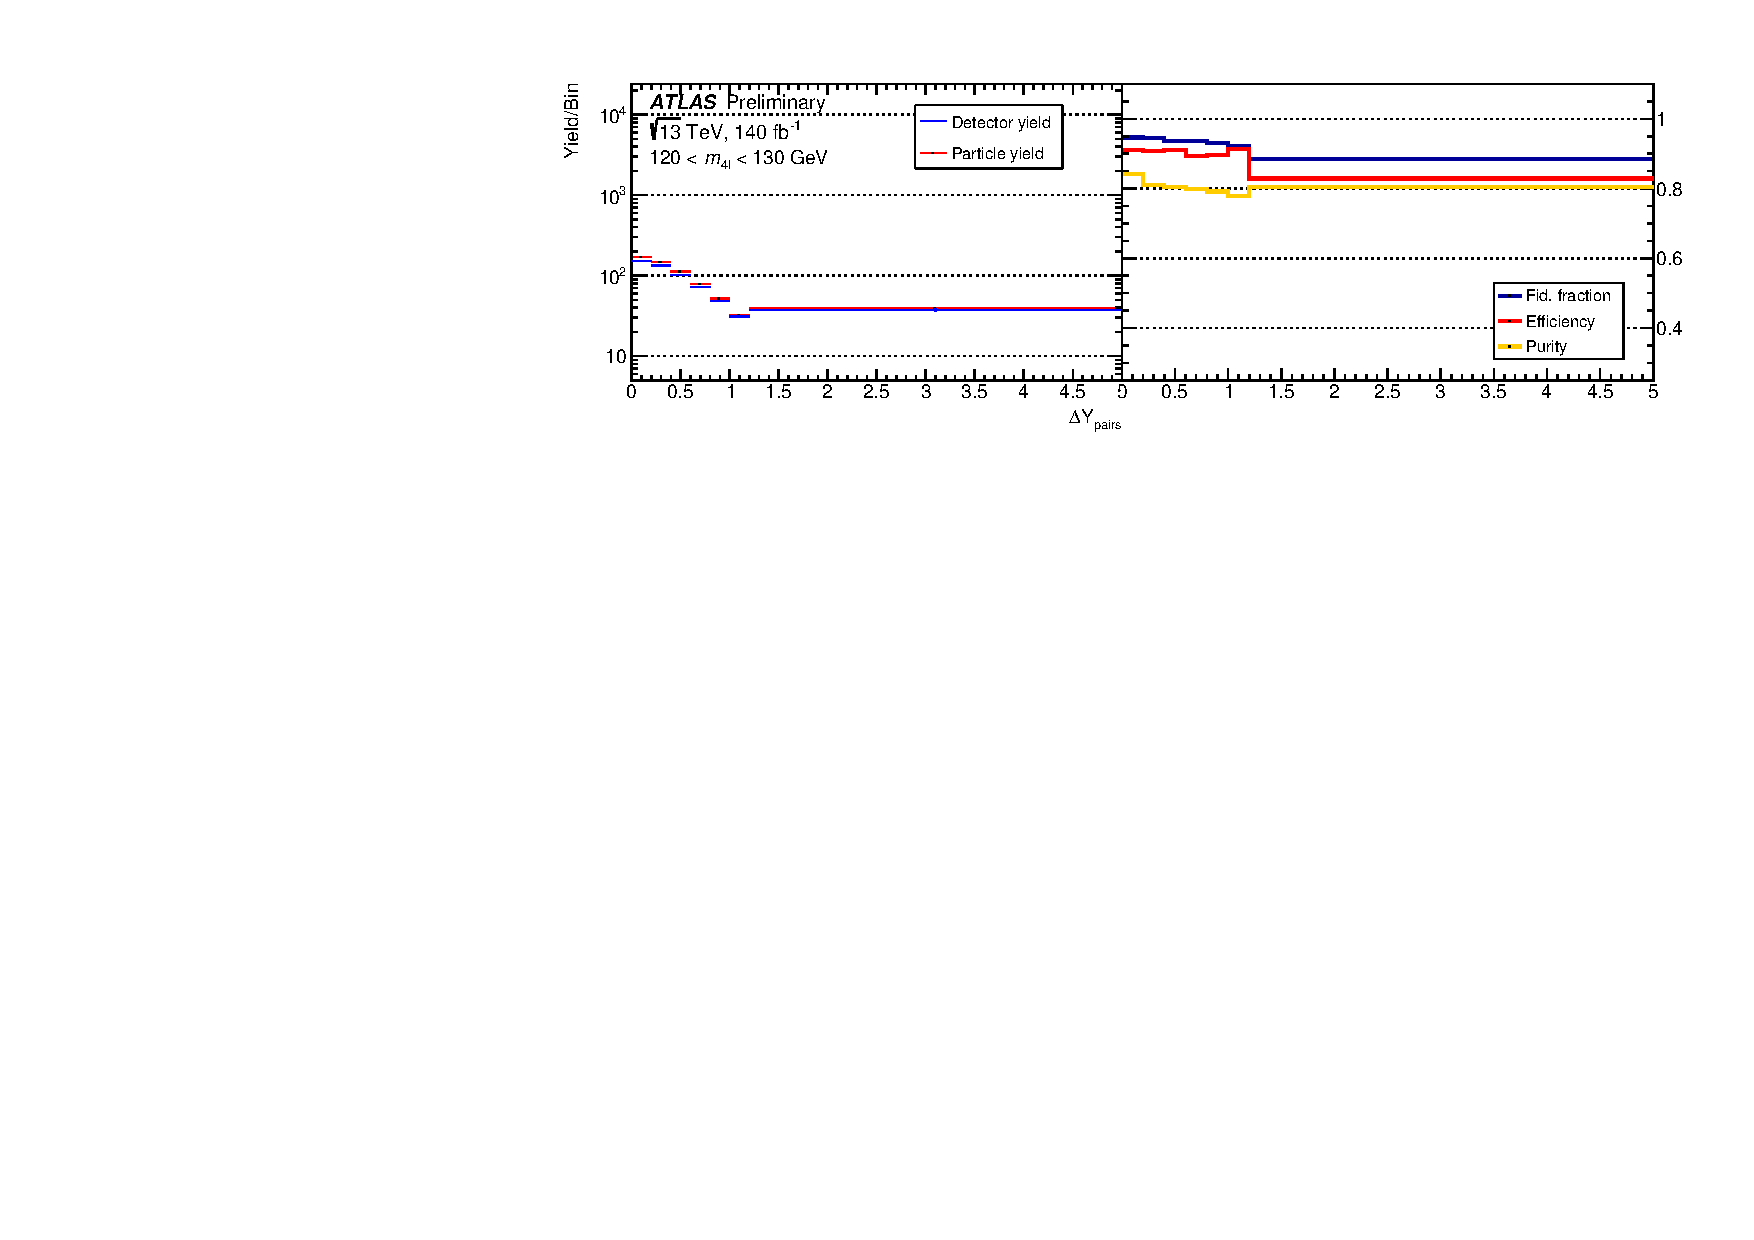
\includegraphics[width = 0.75\textwidth]{Figures/m4l/UnfoldingStudies/v014_inputs/deltaYPairs_m4l120-130inputs.pdf}
    \end{subfigure}
    \begin{subfigure}{.99\textwidth}\centering
        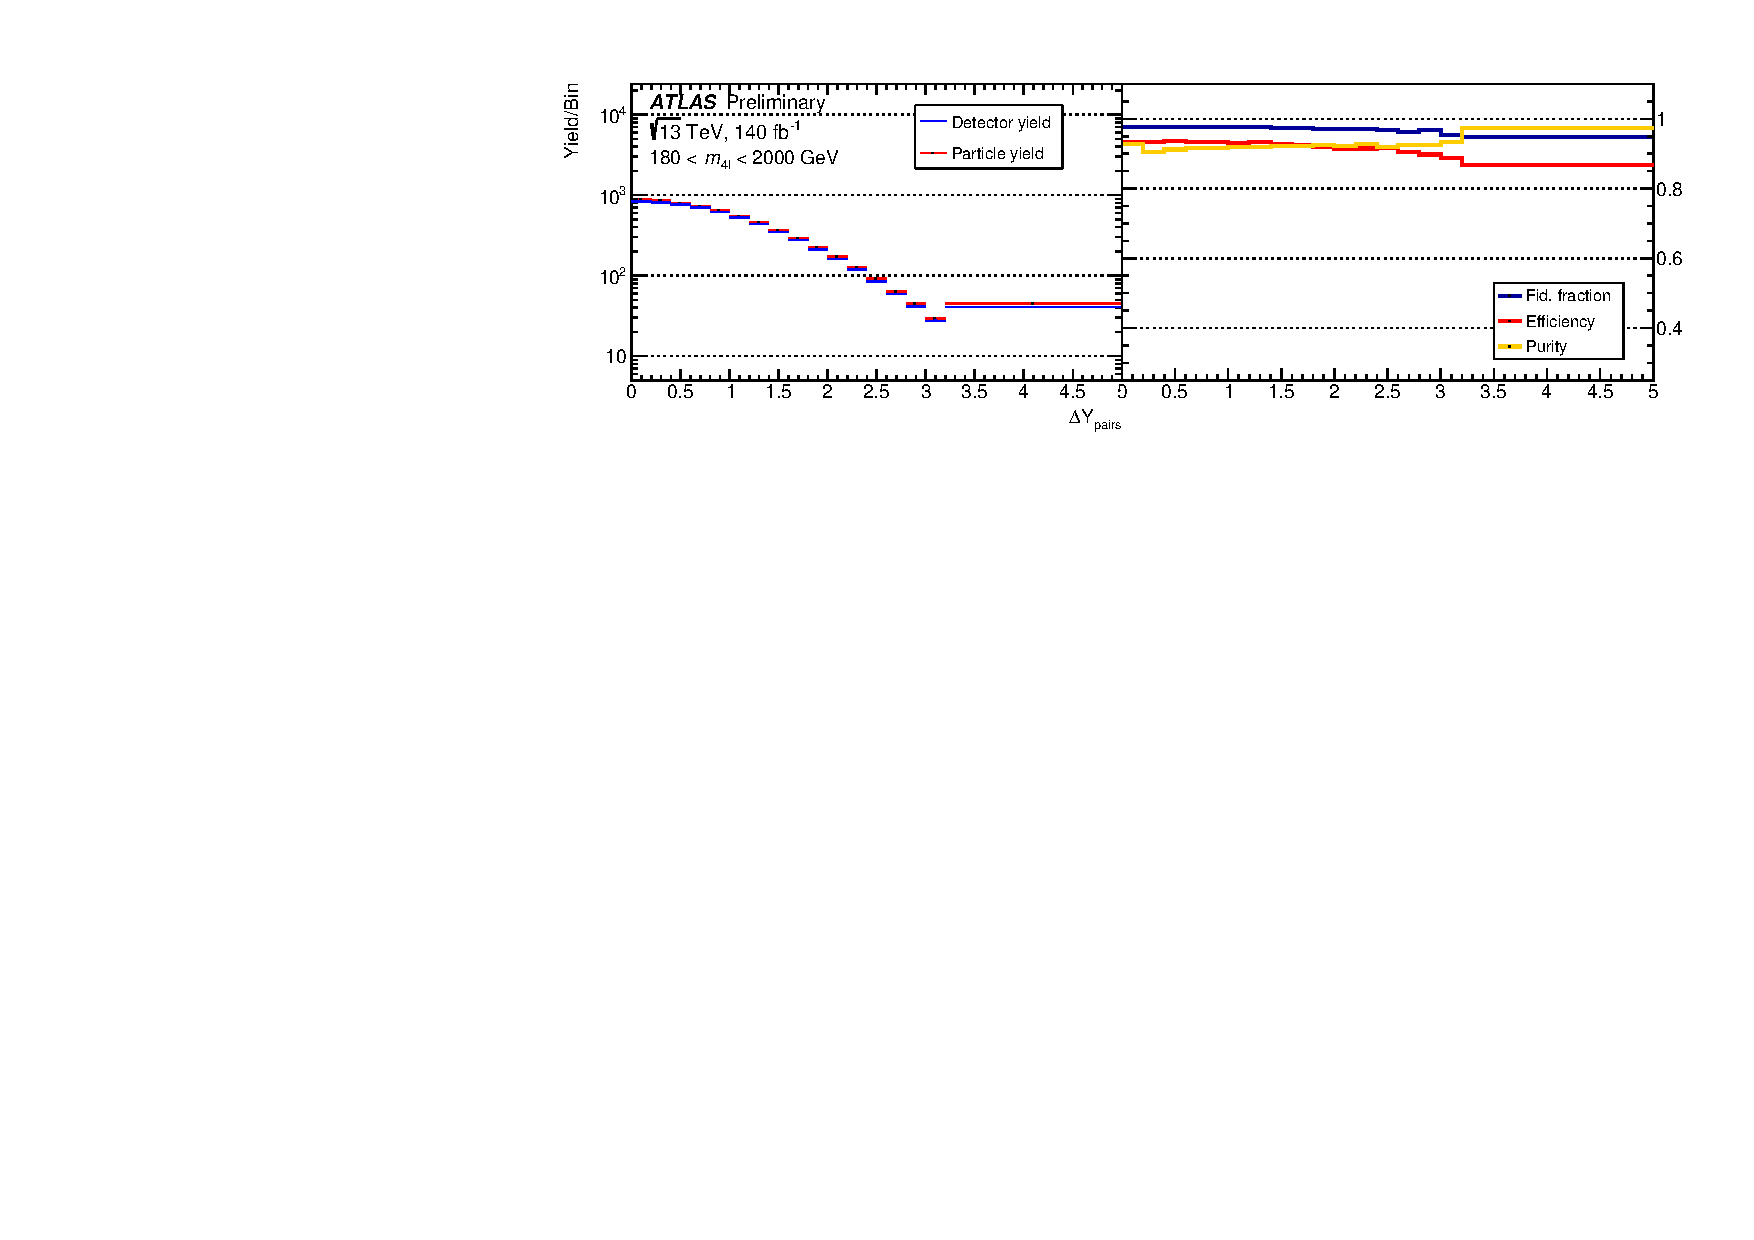
\includegraphics[width = 0.75\textwidth]{Figures/m4l/UnfoldingStudies/v014_inputs/deltaYPairs_m4l180-2000inputs.pdf}
    \end{subfigure}
    \begin{subfigure}{.99\textwidth}\centering
        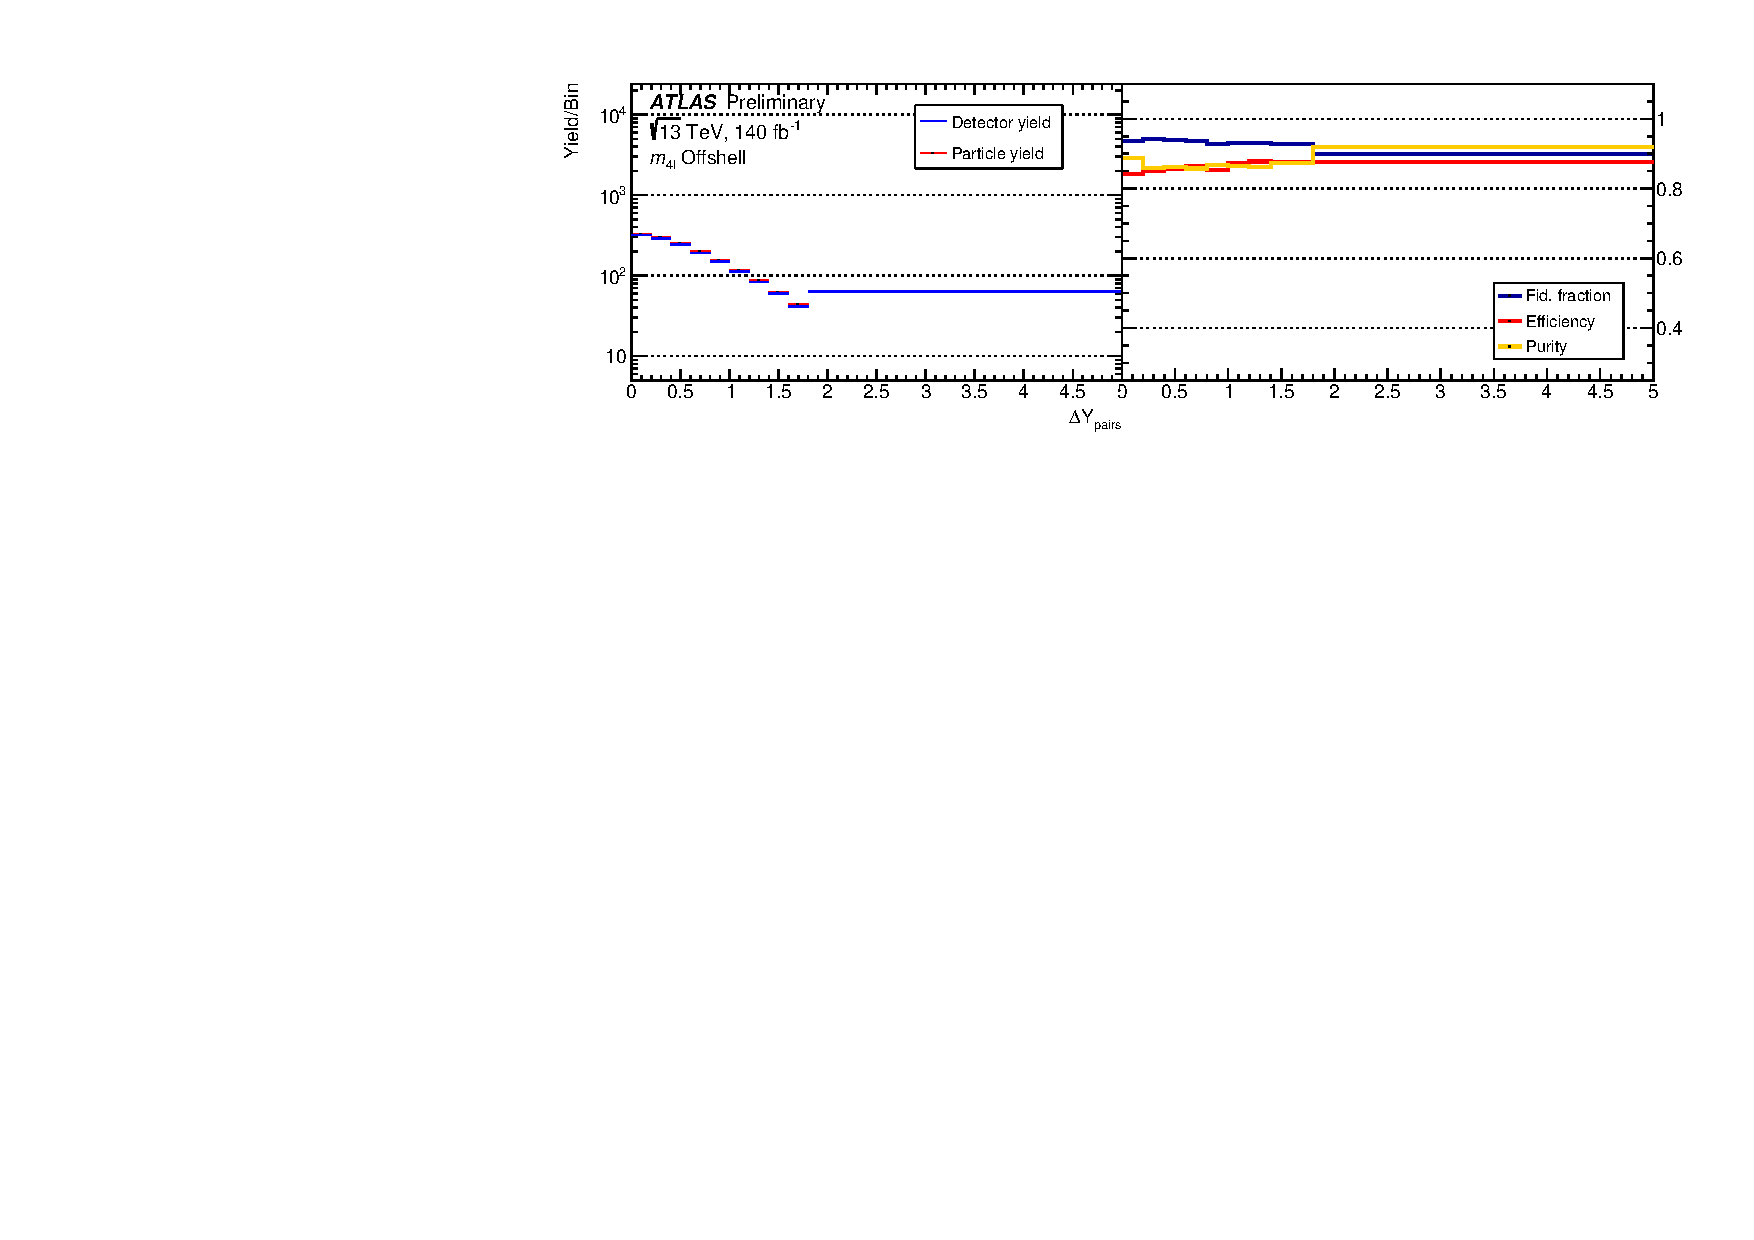
\includegraphics[width = 0.75\textwidth]{Figures/m4l/UnfoldingStudies/v014_inputs/deltaYPairs_m4loffshellinputs.pdf}
    \end{subfigure}
    \caption{In the left-hand panels, the number of predicted events passing the reconstruction- and fiducial- level selections are displayed as the detector yield and particle yield, respectively. The right-hand panel shows the efficiency, fiducial purity and fiducial fraction. All variables are plotted as a function of the \dYPairs bins, in slices of the \mFourL variable which are stacked and labelled with the included \mFourL range.
    \label{fig:dypunf}}
\end{figure}  

\FloatBarrier
\clearpage

\begin{figure}[htb]
    \centering 
    \begin{subfigure}{.99\textwidth}\centering
        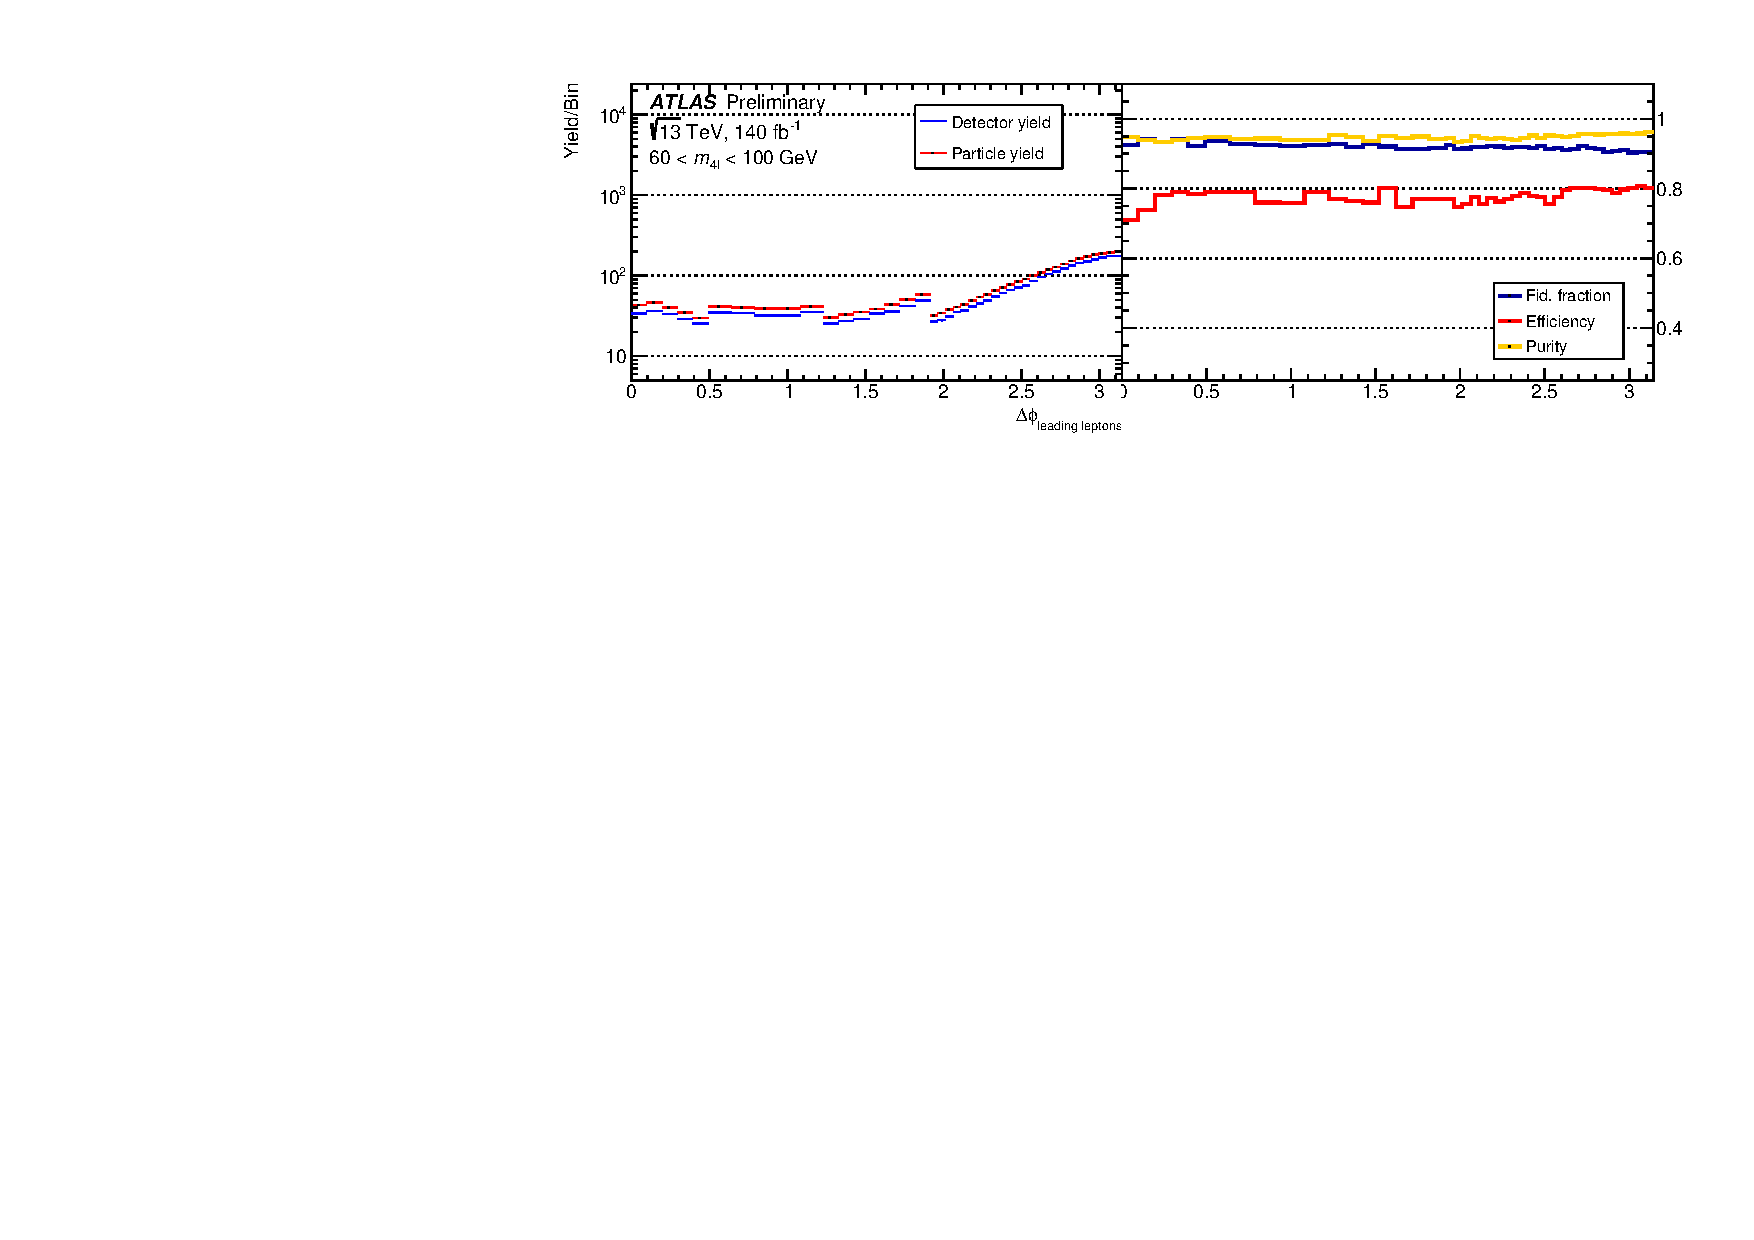
\includegraphics[width = 0.75\textwidth]{Figures/m4l/UnfoldingStudies/v014_inputs/deltaPhiLeadingLeptons_m4l60-100inputs.pdf}
    \end{subfigure}
    \begin{subfigure}{.99\textwidth}\centering
        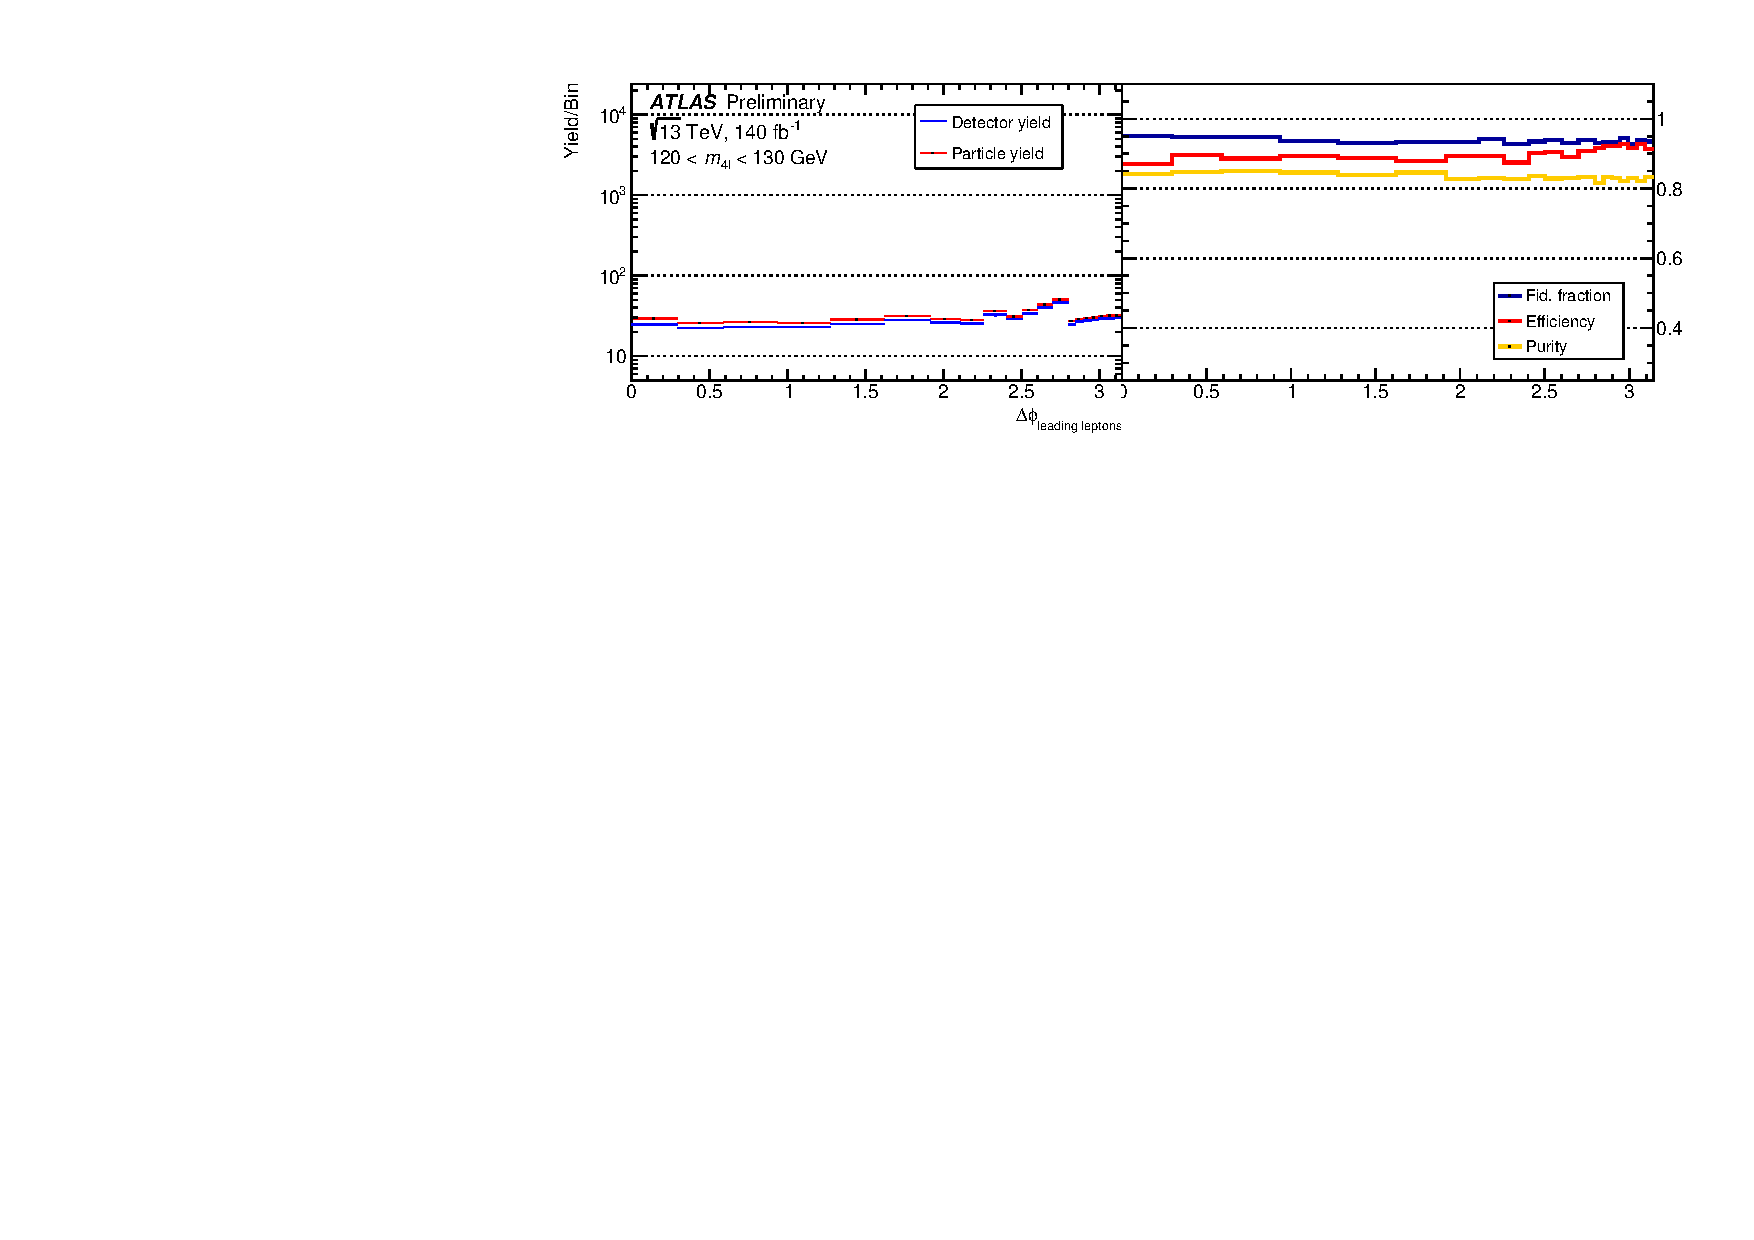
\includegraphics[width = 0.75\textwidth]{Figures/m4l/UnfoldingStudies/v014_inputs/deltaPhiLeadingLeptons_m4l120-130inputs.pdf}
    \end{subfigure}
    \begin{subfigure}{.99\textwidth}\centering
        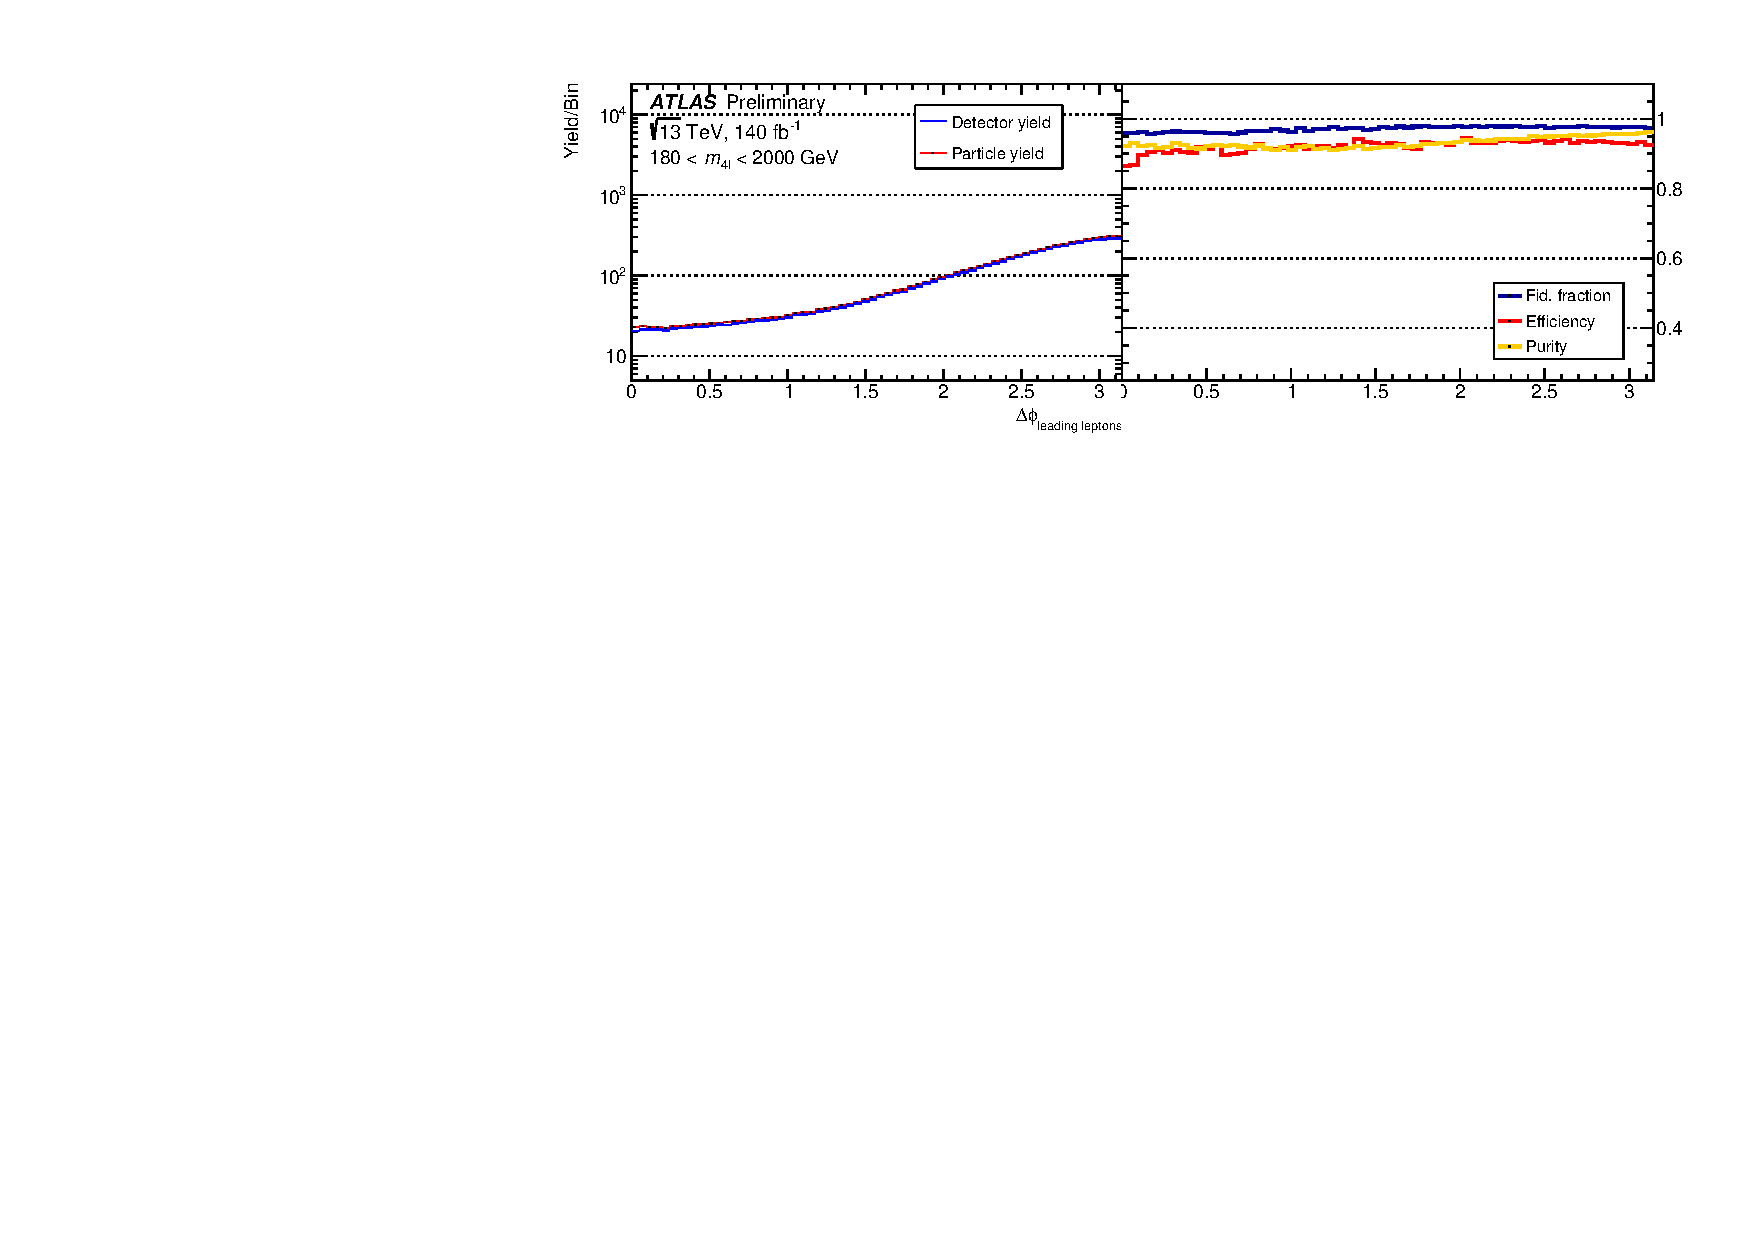
\includegraphics[width = 0.75\textwidth]{Figures/m4l/UnfoldingStudies/v014_inputs/deltaPhiLeadingLeptons_m4l180-2000inputs.pdf}
    \end{subfigure}
    \begin{subfigure}{.99\textwidth}\centering
        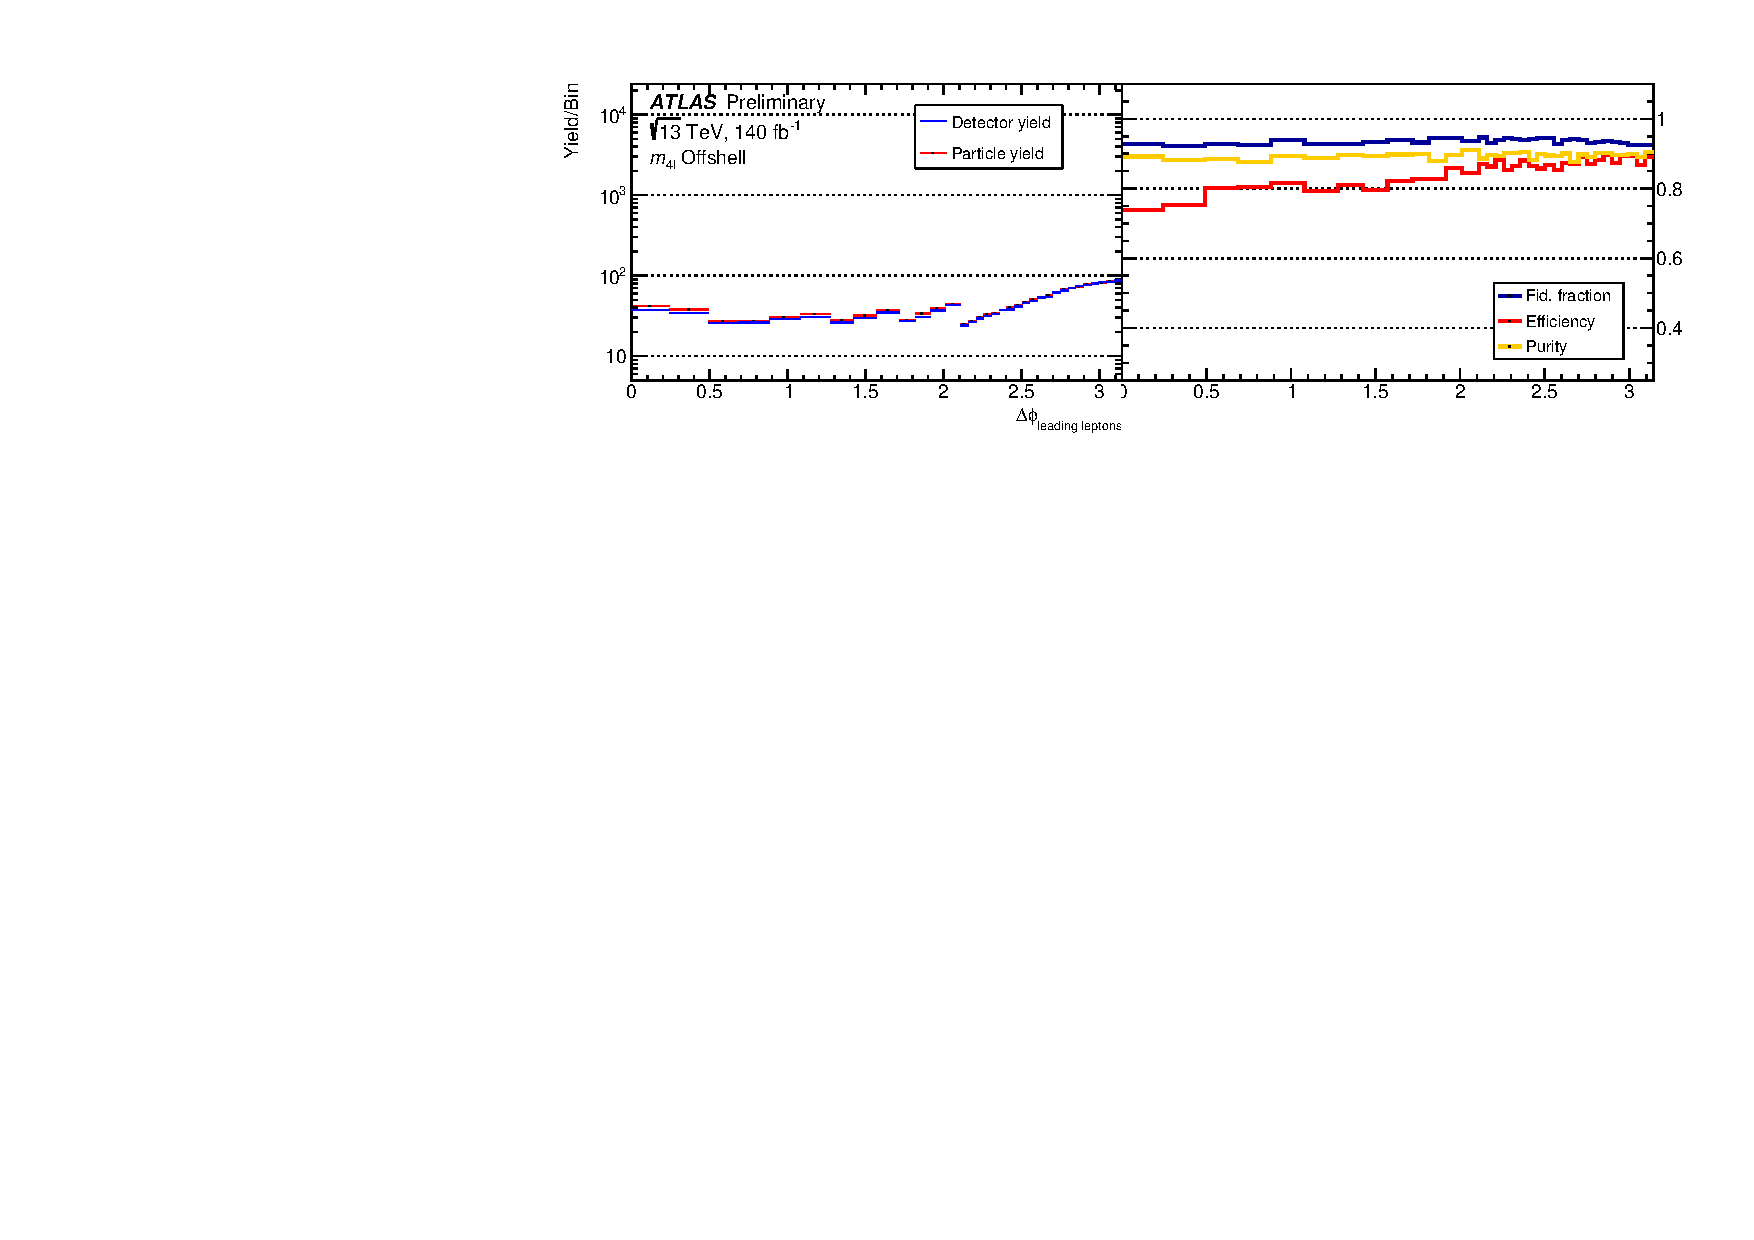
\includegraphics[width = 0.75\textwidth]{Figures/m4l/UnfoldingStudies/v014_inputs/deltaPhiLeadingLeptons_m4loffshellinputs.pdf}
    \end{subfigure}
    \caption{In the left-hand panels, the number of predicted events passing the reconstruction- and fiducial- level selections are displayed as the detector yield and particle yield, respectively. The right-hand panel shows the efficiency, fiducial purity and fiducial fraction. All variables are plotted as a function of the \dPhill bins, in slices of the \mFourL variable which are stacked and labelled with the included \mFourL range.
    \label{fig:dphiunf}}
\end{figure}  

\FloatBarrier
\clearpage

%%%%%%%%%%%%%%%%%%%%Migration matrices %%%%%%%%%%%%%%%%%%%%%%%%%%%%%%%%%%%%%%%
\begin{figure}[htb]
  \centering
  \begin{subfigure}{.65\textwidth}\centering\includegraphics[width = 0.99\textwidth]{Figures/m4l/UnfoldingStudies/v014_matrices/inclusive_vs_m4lMatrix.pdf}\end{subfigure}
 \caption{Migration matrices for the four \mFourL regions between the slices. \label{fig:inclvm4lmat}}
\end{figure}

%%%%%%%%%%%%%%%%%%%%Migration matrices %%%%%%%%%%%%%%%%%%%%%%%%%%%%%%%%%%%%%%%
\begin{figure}[htb]
  \centering
  \begin{subfigure}{.49\textwidth}\centering\includegraphics[width = 0.95\textwidth]{Figures/m4l/UnfoldingStudies/v014_matrices/m4l_pt4l0-10Matrix.pdf}\end{subfigure}
  \begin{subfigure}{.49\textwidth}\centering\includegraphics[width = 0.95\textwidth]{Figures/m4l/UnfoldingStudies/v014_matrices/m4l_pt4l10-20Matrix.pdf}\end{subfigure}
  \begin{subfigure}{.49\textwidth}\centering\includegraphics[width = 0.95\textwidth]{Figures/m4l/UnfoldingStudies/v014_matrices/m4l_pt4l20-50Matrix.pdf}\end{subfigure}
  \begin{subfigure}{.49\textwidth}\centering\includegraphics[width = 0.95\textwidth]{Figures/m4l/UnfoldingStudies/v014_matrices/m4l_pt4l50-100Matrix.pdf}\end{subfigure}
  \begin{subfigure}{.49\textwidth}\centering\includegraphics[width = 0.95\textwidth]{Figures/m4l/UnfoldingStudies/v014_matrices/m4l_pt4l100-600Matrix.pdf}\end{subfigure}
  \begin{subfigure}{.49\textwidth}\centering\includegraphics[width = 0.95\textwidth]{Figures/m4l/UnfoldingStudies/v014_matrices/m4l_pt4lMatrix.pdf}\end{subfigure}
 \caption{Migration matrices for the \mFourL bins in each \ptFourL slice of the \mFourL-\ptFourL distribution and between the slices.\label{fig:pt4lmat}}
\end{figure}

%%%%%%%%%%%%%%%%%%%%Migration matrices %%%%%%%%%%%%%%%%%%%%%%%%%%%%%%%%%%%%%%%

\begin{figure}[htb]
  \centering
  \begin{subfigure}{.49\textwidth}\centering\includegraphics[width = 0.95\textwidth]{Figures/m4l/UnfoldingStudies/v014_matrices/m4l_y4l0-3Matrix.pdf}\end{subfigure}
  \begin{subfigure}{.49\textwidth}\centering\includegraphics[width = 0.95\textwidth]{Figures/m4l/UnfoldingStudies/v014_matrices/m4l_y4l3-6Matrix.pdf}\end{subfigure}
  \begin{subfigure}{.49\textwidth}\centering\includegraphics[width = 0.95\textwidth]{Figures/m4l/UnfoldingStudies/v014_matrices/m4l_y4l6-9Matrix.pdf}\end{subfigure}
  \begin{subfigure}{.49\textwidth}\centering\includegraphics[width = 0.95\textwidth]{Figures/m4l/UnfoldingStudies/v014_matrices/m4l_y4l9-12Matrix.pdf}\end{subfigure}
  \begin{subfigure}{.49\textwidth}\centering\includegraphics[width = 0.95\textwidth]{Figures/m4l/UnfoldingStudies/v014_matrices/m4l_y4l12-25Matrix.pdf}\end{subfigure}
 \begin{subfigure}{.49\textwidth}\centering\includegraphics[width = 0.95\textwidth]{Figures/m4l/UnfoldingStudies/v014_matrices/m4l_y4lMatrix.pdf}\end{subfigure}
\caption{Migration matrices for the \mFourL bins in each \yFourL slice of the \mFourL-\yFourL distribution and between the slices.}
 \end{figure}

\FloatBarrier
\clearpage
%flavours

\begin{figure}[htb]
  \centering
  \begin{subfigure}{.49\textwidth}\centering\includegraphics[width = 0.95\textwidth]{Figures/m4l/UnfoldingStudies/v014_matrices/m4l_event_type0-1Matrix.pdf}\end{subfigure}
  \begin{subfigure}{.49\textwidth}\centering\includegraphics[width = 0.95\textwidth]{Figures/m4l/UnfoldingStudies/v014_matrices/m4l_event_type0-0Matrix.pdf}\end{subfigure}
  \begin{subfigure}{.49\textwidth}\centering\includegraphics[width = 0.95\textwidth]{Figures/m4l/UnfoldingStudies/v014_matrices/m4l_event_type1-3Matrix.pdf}\end{subfigure}
 \begin{subfigure}{.49\textwidth}\centering\includegraphics[width = 0.95\textwidth]{Figures/m4l/UnfoldingStudies/v014_matrices/m4l_event_typeMatrix.pdf}\end{subfigure}
\caption{Migration matrices for the \mFourL bins in each flavour slice and  between the flavour slices of the \mFourL-lepton flavour distribution (where no migration is seen, as expected).}
 \end{figure}

%%%%%%%%%%%%%%%%%%%%Migration matrices %%%%%%%%%%%%%%%%%%%%%%%%%%%%%%%%%%%%%%%

\begin{figure}[htb]
  \centering
  \begin{subfigure}{.49\textwidth}\centering\includegraphics[width = 0.95\textwidth]{Figures/m4l/UnfoldingStudies/v014_matrices/m12_m4l60-100Matrix.pdf}\end{subfigure}
  \begin{subfigure}{.49\textwidth}\centering\includegraphics[width = 0.95\textwidth]{Figures/m4l/UnfoldingStudies/v014_matrices/m12_m4l120-130Matrix.pdf}\end{subfigure}
  \begin{subfigure}{.49\textwidth}\centering\includegraphics[width = 0.95\textwidth]{Figures/m4l/UnfoldingStudies/v014_matrices/m12_m4l180-2000Matrix.pdf}\end{subfigure}
  \begin{subfigure}{.49\textwidth}\centering\includegraphics[width = 0.95\textwidth]{Figures/m4l/UnfoldingStudies/v014_matrices/m12_m4loffshellMatrix.pdf}\end{subfigure}
 \begin{subfigure}{.49\textwidth}\centering\includegraphics[width = 0.95\textwidth]{Figures/m4l/UnfoldingStudies/v014_matrices/m12_m4lMatrix.pdf}\end{subfigure}
\caption{Migration matrices for the \mZOne bins in each of the \mFourL slices of the \mZOne-\mFourL distribution and between the slices.}
 \end{figure}


%%%%%%%%%%%%%%%%%%%%Migration matrices %%%%%%%%%%%%%%%%%%%%%%%%%%%%%%%%%%%%%%%

\begin{figure}[htb]
  \centering
  \begin{subfigure}{.49\textwidth}\centering\includegraphics[width = 0.95\textwidth]{Figures/m4l/UnfoldingStudies/v014_matrices/m34_m4l60-100Matrix.pdf}\end{subfigure}
  \begin{subfigure}{.49\textwidth}\centering\includegraphics[width = 0.95\textwidth]{Figures/m4l/UnfoldingStudies/v014_matrices/m34_m4l120-130Matrix.pdf}\end{subfigure}
  \begin{subfigure}{.49\textwidth}\centering\includegraphics[width = 0.95\textwidth]{Figures/m4l/UnfoldingStudies/v014_matrices/m34_m4l180-2000Matrix.pdf}\end{subfigure}
  \begin{subfigure}{.49\textwidth}\centering\includegraphics[width = 0.95\textwidth]{Figures/m4l/UnfoldingStudies/v014_matrices/m34_m4loffshellMatrix.pdf}\end{subfigure}
  \begin{subfigure}{.49\textwidth}\centering\includegraphics[width = 0.95\textwidth]{Figures/m4l/UnfoldingStudies/v014_matrices/m34_m4lMatrix.pdf}\end{subfigure}
\caption{Migration matrices for the \mZTwo bins in each of the \mFourL slices of the \mZTwo-\mFourL distribution and between the slices.}
 \end{figure}


%%%%%%%%%%%%%%%%%%%%Migration matrices %%%%%%%%%%%%%%%%%%%%%%%%%%%%%%%%%%%%%%%

\begin{figure}[htb]
  \centering
  \begin{subfigure}{.49\textwidth}\centering\includegraphics[width = 0.95\textwidth]{Figures/m4l/UnfoldingStudies/v014_matrices/pt12_m4l60-100Matrix.pdf}\end{subfigure}
  \begin{subfigure}{.49\textwidth}\centering\includegraphics[width = 0.95\textwidth]{Figures/m4l/UnfoldingStudies/v014_matrices/pt12_m4l120-130Matrix.pdf}\end{subfigure}
  \begin{subfigure}{.49\textwidth}\centering\includegraphics[width = 0.95\textwidth]{Figures/m4l/UnfoldingStudies/v014_matrices/pt12_m4l180-2000Matrix.pdf}\end{subfigure}
  \begin{subfigure}{.49\textwidth}\centering\includegraphics[width = 0.95\textwidth]{Figures/m4l/UnfoldingStudies/v014_matrices/pt12_m4loffshellMatrix.pdf}\end{subfigure}
  \begin{subfigure}{.49\textwidth}\centering\includegraphics[width = 0.95\textwidth]{Figures/m4l/UnfoldingStudies/v014_matrices/pt12_m4lMatrix.pdf}\end{subfigure}
\caption{Migration matrices for the \ptZOne bins in each of the \mFourL slices of the \ptZOne-\mFourL distribution and between the slices.}
 \end{figure}

\FloatBarrier
\clearpage

%%%%%%%%%%%%%%%%%%%%Migration matrices %%%%%%%%%%%%%%%%%%%%%%%%%%%%%%%%%%%%%%%

\begin{figure}[htb]
  \centering
  \begin{subfigure}{.49\textwidth}\centering\includegraphics[width = 0.95\textwidth]{Figures/m4l/UnfoldingStudies/v014_matrices/pt34_m4l60-100Matrix.pdf}\end{subfigure}
  \begin{subfigure}{.49\textwidth}\centering\includegraphics[width = 0.95\textwidth]{Figures/m4l/UnfoldingStudies/v014_matrices/pt34_m4l120-130Matrix.pdf}\end{subfigure}
  \begin{subfigure}{.49\textwidth}\centering\includegraphics[width = 0.95\textwidth]{Figures/m4l/UnfoldingStudies/v014_matrices/pt34_m4l180-2000Matrix.pdf}\end{subfigure}
  \begin{subfigure}{.49\textwidth}\centering\includegraphics[width = 0.95\textwidth]{Figures/m4l/UnfoldingStudies/v014_matrices/pt34_m4loffshellMatrix.pdf}\end{subfigure}
  \begin{subfigure}{.49\textwidth}\centering\includegraphics[width = 0.95\textwidth]{Figures/m4l/UnfoldingStudies/v014_matrices/pt34_m4lMatrix.pdf}\end{subfigure}
\caption{Migration matrices of the \ptZTwo bins in each of the \mFourL slices of the \ptZTwo-\mFourL distribution and between the slices.}
 \end{figure}


%%%%%%%%%%%%%%%%%%%%Migration matrices %%%%%%%%%%%%%%%%%%%%%%%%%%%%%%%%%%%%%%%

\begin{figure}[htb]
  \centering
  \begin{subfigure}{.49\textwidth}\centering\includegraphics[width = 0.95\textwidth]{Figures/m4l/UnfoldingStudies/v014_matrices/cosThetaStar1_m4l60-100Matrix.pdf}\end{subfigure}
  \begin{subfigure}{.49\textwidth}\centering\includegraphics[width = 0.95\textwidth]{Figures/m4l/UnfoldingStudies/v014_matrices/cosThetaStar1_m4l120-130Matrix.pdf}\end{subfigure}
  \begin{subfigure}{.49\textwidth}\centering\includegraphics[width = 0.95\textwidth]{Figures/m4l/UnfoldingStudies/v014_matrices/cosThetaStar1_m4l180-2000Matrix.pdf}\end{subfigure}
  \begin{subfigure}{.49\textwidth}\centering\includegraphics[width = 0.95\textwidth]{Figures/m4l/UnfoldingStudies/v014_matrices/cosThetaStar1_m4loffshellMatrix.pdf}\end{subfigure}
  \begin{subfigure}{.49\textwidth}\centering\includegraphics[width = 0.95\textwidth]{Figures/m4l/UnfoldingStudies/v014_matrices/cosThetaStar1_m4lMatrix.pdf}\end{subfigure}
\caption{Migration matrices for the $\thetastar_{1}$ bins in each of the \mFourL slices of the $\thetastar_{1}$-\mFourL distribution and between the slices.}
 \end{figure}


%%%%%%%%%%%%%%%%%%%%Migration matrices %%%%%%%%%%%%%%%%%%%%%%%%%%%%%%%%%%%%%%%

\begin{figure}[htb]
  \centering
  \begin{subfigure}{.49\textwidth}\centering\includegraphics[width = 0.95\textwidth]{Figures/m4l/UnfoldingStudies/v014_matrices/cosThetaStar3_m4l60-100Matrix.pdf}\end{subfigure}
  \begin{subfigure}{.49\textwidth}\centering\includegraphics[width = 0.95\textwidth]{Figures/m4l/UnfoldingStudies/v014_matrices/cosThetaStar3_m4l120-130Matrix.pdf}\end{subfigure}
  \begin{subfigure}{.49\textwidth}\centering\includegraphics[width = 0.95\textwidth]{Figures/m4l/UnfoldingStudies/v014_matrices/cosThetaStar3_m4l180-2000Matrix.pdf}\end{subfigure}
  \begin{subfigure}{.49\textwidth}\centering\includegraphics[width = 0.95\textwidth]{Figures/m4l/UnfoldingStudies/v014_matrices/cosThetaStar3_m4loffshellMatrix.pdf}\end{subfigure}
  \begin{subfigure}{.49\textwidth}\centering\includegraphics[width = 0.95\textwidth]{Figures/m4l/UnfoldingStudies/v014_matrices/cosThetaStar3_m4lMatrix.pdf}\end{subfigure}
\caption{Migration matrices for the $\thetastar_{2}$ bins in each of the \mFourL slices of the $\thetastar_{2}$-\mFourL distribution and between the slices.}
 \end{figure}

\FloatBarrier

%%%%%%%%%%%%%%%%%%%%Migration matrices %%%%%%%%%%%%%%%%%%%%%%%%%%%%%%%%%%%%%%%

\begin{figure}[htb]
  \centering
  \begin{subfigure}{.49\textwidth}\centering\includegraphics[width = 0.95\textwidth]{Figures/m4l/UnfoldingStudies/v014_matrices/deltaPhiPairs_m4l60-100Matrix.pdf}\end{subfigure}
  \begin{subfigure}{.49\textwidth}\centering\includegraphics[width = 0.95\textwidth]{Figures/m4l/UnfoldingStudies/v014_matrices/deltaPhiPairs_m4l120-130Matrix.pdf}\end{subfigure}
  \begin{subfigure}{.49\textwidth}\centering\includegraphics[width = 0.95\textwidth]{Figures/m4l/UnfoldingStudies/v014_matrices/deltaPhiPairs_m4l180-2000Matrix.pdf}\end{subfigure}
  \begin{subfigure}{.49\textwidth}\centering\includegraphics[width = 0.95\textwidth]{Figures/m4l/UnfoldingStudies/v014_matrices/deltaPhiPairs_m4loffshellMatrix.pdf}\end{subfigure}
   \begin{subfigure}{.49\textwidth}\centering\includegraphics[width = 0.95\textwidth]{Figures/m4l/UnfoldingStudies/v014_matrices/deltaPhiPairs_m4lMatrix.pdf}\end{subfigure}
%  \begin{subfigure}{.49\textwidth}\centering\includegraphics[width = 0.95\textwidth]{Figures/m4l/UnfoldingStudies/v011_matrices/deltaPhiPairs_m4lMatrix.pdf}\end{subfigure}
\caption{Migration matrix for the \dPhiPairs bins in each of the \mFourL slices of the \dPhiPairs-\mFourL distribution and between the slices.}
 \end{figure}


%%%%%%%%%%%%%%%%%%%%Migration matrices %%%%%%%%%%%%%%%%%%%%%%%%%%%%%%%%%%%%%%%

\begin{figure}[htb]
    \centering
    \begin{subfigure}{.49\textwidth}\centering\includegraphics[width = 0.95\textwidth]{Figures/m4l/UnfoldingStudies/v014_matrices/deltaYPairs_m4l60-100Matrix.pdf}\end{subfigure}
    \begin{subfigure}{.49\textwidth}\centering\includegraphics[width = 0.95\textwidth]{Figures/m4l/UnfoldingStudies/v014_matrices/deltaYPairs_m4l120-130Matrix.pdf}\end{subfigure}
    \begin{subfigure}{.49\textwidth}\centering\includegraphics[width = 0.95\textwidth]{Figures/m4l/UnfoldingStudies/v014_matrices/deltaYPairs_m4l180-2000Matrix.pdf}\end{subfigure}
    \begin{subfigure}{.49\textwidth}\centering\includegraphics[width = 0.95\textwidth]{Figures/m4l/UnfoldingStudies/v014_matrices/deltaYPairs_m4loffshellMatrix.pdf}\end{subfigure}
    \begin{subfigure}{.49\textwidth}\centering\includegraphics[width = 0.95\textwidth]{Figures/m4l/UnfoldingStudies/v014_matrices/deltaYPairs_m4lMatrix.pdf}\end{subfigure}
    %  \begin{subfigure}{.49\textwidth}\centering\includegraphics[width = 0.95\textwidth]{Figures/m4l/UnfoldingStudies/v011_matrices/deltaYPairs_m4lMatrix.pdf}\end{subfigure}
    \caption{Migration matrices for the \dYPairs bins in each of the \mFourL slices of the \dYPairs-\mFourL distribution and between the slices.}
\end{figure}


%%%migration matrices %%%%%%%%%%%%%%%%%%%%%%%%%%%%%%%%%%%%%%%%%%%5

\begin{figure}[htb]
  \centering
  \begin{subfigure}{.49\textwidth}\centering\includegraphics[width = 0.95\textwidth]{Figures/m4l/UnfoldingStudies/v014_matrices/deltaPhiLeadingLeptons_m4l60-100Matrix.pdf}\end{subfigure}
  \begin{subfigure}{.49\textwidth}\centering\includegraphics[width = 0.95\textwidth]{Figures/m4l/UnfoldingStudies/v014_matrices/deltaPhiLeadingLeptons_m4l120-130Matrix.pdf}\end{subfigure}
  \begin{subfigure}{.49\textwidth}\centering\includegraphics[width = 0.95\textwidth]{Figures/m4l/UnfoldingStudies/v014_matrices/deltaPhiLeadingLeptons_m4l180-2000Matrix.pdf}\end{subfigure}
  \begin{subfigure}{.49\textwidth}\centering\includegraphics[width = 0.95\textwidth]{Figures/m4l/UnfoldingStudies/v014_matrices/deltaPhiLeadingLeptons_m4loffshellMatrix.pdf}\end{subfigure}
  \begin{subfigure}{.49\textwidth}\centering\includegraphics[width = 0.95\textwidth]{Figures/m4l/UnfoldingStudies/v014_matrices/deltaPhiLeadingLeptons_m4lMatrix.pdf}\end{subfigure}
%  \begin{subfigure}{.49\textwidth}\centering\includegraphics[width = 0.95\textwidth]{Figures/m4l/UnfoldingStudies/v011_matrices/deltaPhiLeadingLeptons_m4lMatrix.pdf}\end{subfigure}
\caption{Migration matrices for the \dPhill bins in each of the \mFourL slices of the \dPhill-\mFourL distribution and between the slices.\label{fig:dphimat}}
 \end{figure}
%%

%%%%%%%%%%%%%%%%%%%%%%%%%%%%Full MC closure test %%%%%%%%%%%%%%%%%%%%%%%%%%%%%%%%%%%%%%%%%%%%%%%%%%%%%%%%%%
\FloatBarrier
\begin{figure}[htb]
  \centering
  \begin{subfigure}{.65\textwidth}\centering\includegraphics[width = 0.99\textwidth]{Figures/m4l/UnfoldingStudies/v014_closure/FullMCClosure_m4l_pt4l.pdf}\end{subfigure}
\caption{MC cross-check closure test for all bins of the inclusive \mFourL-\ptFourL distribution.\label{fig:pt4lclos}}
 \end{figure}

\begin{figure}[htb]
  \centering
  \begin{subfigure}{.65\textwidth}\centering\includegraphics[width = 0.99\textwidth]{Figures/m4l/UnfoldingStudies/v014_closure/FullMCClosure_m4l_y4l.pdf}\end{subfigure}
\caption{MC cross-check closure test for all bins of the inclusive \mFourL-\yFourL distribution.}
 \end{figure}

\begin{figure}[htb]
  \centering
  \begin{subfigure}{.65\textwidth}\centering\includegraphics[width = 0.99\textwidth]{Figures/m4l/UnfoldingStudies/v014_closure/FullMCClosure_m4l_event_type.pdf}\end{subfigure}
\caption{MC cross-check closure test for all bins of the inclusive \mFourL-channel distribution.}
 \end{figure}

\begin{figure}[htb]
  \centering
  \begin{subfigure}{.65\textwidth}\centering\includegraphics[width = 0.99\textwidth]{Figures/m4l/UnfoldingStudies/v014_closure/FullMCClosure_m12_m4l.pdf}\end{subfigure}
\caption{MC cross-check closure test for all bins of the inclusive \mZOne-\mFourL distribution.}
 \end{figure}

\begin{figure}[htb]
  \centering
  \begin{subfigure}{.65\textwidth}\centering\includegraphics[width = 0.99\textwidth]{Figures/m4l/UnfoldingStudies/v014_closure/FullMCClosure_m34_m4l.pdf}\end{subfigure}
\caption{MC cross-check closure test for all bins of the inclusive \mZTwo-\mFourL distribution.}
 \end{figure}

\begin{figure}[htb]
  \centering
  \begin{subfigure}{.65\textwidth}\centering\includegraphics[width = 0.99\textwidth]{Figures/m4l/UnfoldingStudies/v014_closure/FullMCClosure_pt12_m4l.pdf}\end{subfigure}
\caption{MC cross-check closure test for all bins of the inclusive \ptZOne-\mFourL distribution.}
 \end{figure}

\begin{figure}[htb]
  \centering
  \begin{subfigure}{.65\textwidth}\centering\includegraphics[width = 0.99\textwidth]{Figures/m4l/UnfoldingStudies/v014_closure/FullMCClosure_pt34_m4l.pdf}\end{subfigure}
\caption{MC cross-check closure test for all bins of the inclusive \ptZTwo-\mFourL distribution.}
 \end{figure}

\begin{figure}[htb]
  \centering
  \begin{subfigure}{.65\textwidth}\centering\includegraphics[width = 0.99\textwidth]{Figures/m4l/UnfoldingStudies/v014_closure/FullMCClosure_cosThetaStar1_m4l.pdf}\end{subfigure}
\caption{MC cross-check closure test for all bins of the inclusive \costhetastar-\mFourL distribution.}
 \end{figure}

\begin{figure}[htb]
  \centering
  \begin{subfigure}{.65\textwidth}\centering\includegraphics[width = 0.99\textwidth]{Figures/m4l/UnfoldingStudies/v014_closure/FullMCClosure_cosThetaStar3_m4l.pdf}\end{subfigure}
\caption{MC cross-check closure test for all bins of the inclusive \costhetastar-\mFourL distribution.}
 \end{figure}

\begin{figure}[htb]
  \centering
  \begin{subfigure}{.65\textwidth}\centering\includegraphics[width = 0.99\textwidth]{Figures/m4l/UnfoldingStudies/v014_closure/FullMCClosure_deltaPhiPairs_m4l.pdf}\end{subfigure}
\caption{MC cross-check closure test for all bins of the inclusive \dPhiPairs-\mFourL distribution.}
 \end{figure}

\begin{figure}[htb]
  \centering
  \begin{subfigure}{.65\textwidth}\centering\includegraphics[width = 0.99\textwidth]{Figures/m4l/UnfoldingStudies/v014_closure/FullMCClosure_deltaYPairs_m4l.pdf}\end{subfigure}
\caption{MC cross-check closure test for all bins of the inclusive \dYPairs-\mFourL distribution.}
 \end{figure}

\begin{figure}[htb]
  \centering
  \begin{subfigure}{.65\textwidth}\centering\includegraphics[width = 0.99\textwidth]{Figures/m4l/UnfoldingStudies/v014_closure/FullMCClosure_deltaPhiLeadingLeptons_m4l.pdf}\end{subfigure}
\caption{MC cross-check closure test for all bins of the inclusive \dPhill-\mFourL distribution.\label{fig:dphiclos}}
 \end{figure}
%%%%%%%%%%%%%%%%%%%%%%%%%%%%50/50 closure %%%%%%%%%%%%%%%%%%%%%%%%%%%%%%%%%%%%%%%%%%%%%%%%%%%%%%%%%%%%%%%%%%%%%%%%%%%%5

\begin{figure}[htb]
  \centering
  \begin{subfigure}{.65\textwidth}\centering\includegraphics[width = 0.99\textwidth]{Figures/m4l/UnfoldingStudies/v014_closure/HalfMCClosure_withPull_m4l_pt4l.pdf}\end{subfigure}
\caption{MC closure test for all bins of the inclusive \mFourL-\ptFourL distribution.\label{fig:pt4lhalf}}
 \end{figure}

\begin{figure}[htb]
  \centering
  \begin{subfigure}{.65\textwidth}\centering\includegraphics[width = 0.99\textwidth]{Figures/m4l/UnfoldingStudies/v014_closure/HalfMCClosure_withPull_m4l_y4l.pdf}\end{subfigure}
\caption{MC closure test for all bins of the inclusive \mFourL-\yFourL distribution.}
 \end{figure}

\begin{figure}[htb]
  \centering
  \begin{subfigure}{.65\textwidth}\centering\includegraphics[width = 0.99\textwidth]{Figures/m4l/UnfoldingStudies/v014_closure/HalfMCClosure_withPull_m4l_event_type.pdf}\end{subfigure}
\caption{MC closure test for all bins of the inclusive \mFourL-channel distribution.}
 \end{figure}

\begin{figure}[htb]
  \centering
  \begin{subfigure}{.65\textwidth}\centering\includegraphics[width = 0.99\textwidth]{Figures/m4l/UnfoldingStudies/v014_closure/HalfMCClosure_withPull_m12_m4l.pdf}\end{subfigure}
\caption{MC closure test for all bins of the inclusive \mZOne-\mFourL distribution.}
 \end{figure}

\begin{figure}[htb]
  \centering
  \begin{subfigure}{.65\textwidth}\centering\includegraphics[width = 0.99\textwidth]{Figures/m4l/UnfoldingStudies/v014_closure/HalfMCClosure_withPull_m34_m4l.pdf}\end{subfigure}
\caption{MC closure test for all bins of the inclusive \mZTwo-\mFourL distribution.}
 \end{figure}

\begin{figure}[htb]
  \centering
  \begin{subfigure}{.65\textwidth}\centering\includegraphics[width = 0.99\textwidth]{Figures/m4l/UnfoldingStudies/v014_closure/HalfMCClosure_withPull_pt12_m4l.pdf}\end{subfigure}
\caption{MC closure test for all bins of the inclusive \ptZOne-\mFourL distribution.}
 \end{figure}

\begin{figure}[htb]
  \centering
  \begin{subfigure}{.65\textwidth}\centering\includegraphics[width = 0.99\textwidth]{Figures/m4l/UnfoldingStudies/v014_closure/HalfMCClosure_withPull_pt34_m4l.pdf}\end{subfigure}
\caption{MC closure test for all bins of the inclusive \ptZTwo-\mFourL distribution.}
 \end{figure}

\begin{figure}[htb]
  \centering
  \begin{subfigure}{.65\textwidth}\centering\includegraphics[width = 0.99\textwidth]{Figures/m4l/UnfoldingStudies/v014_closure/HalfMCClosure_withPull_cosThetaStar1_m4l.pdf}\end{subfigure}
\caption{MC closure test for all bins of the inclusive \costhetastar-\mFourL distribution.}
 \end{figure}

\begin{figure}[htb]
  \centering
  \begin{subfigure}{.65\textwidth}\centering\includegraphics[width = 0.99\textwidth]{Figures/m4l/UnfoldingStudies/v014_closure/HalfMCClosure_withPull_cosThetaStar3_m4l.pdf}\end{subfigure}
\caption{MC closure test for all bins of the inclusive \costhetastar-\mFourL distribution.}
 \end{figure}

\begin{figure}[htb]
  \centering
  \begin{subfigure}{.65\textwidth}\centering\includegraphics[width = 0.99\textwidth]{Figures/m4l/UnfoldingStudies/v014_closure/HalfMCClosure_withPull_deltaPhiPairs_m4l.pdf}\end{subfigure}
\caption{MC closure test for all bins of the inclusive \dPhiPairs-\mFourL distribution.}
 \end{figure}

\begin{figure}[htb]
  \centering
  \begin{subfigure}{.65\textwidth}\centering\includegraphics[width = 0.99\textwidth]{Figures/m4l/UnfoldingStudies/v014_closure/HalfMCClosure_withPull_deltaYPairs_m4l.pdf}\end{subfigure}
\caption{MC closure test for all bins of the inclusive \dYPairs-\mFourL distribution.}
 \end{figure}

\begin{figure}[htb]
  \centering
  \begin{subfigure}{.65\textwidth}\centering\includegraphics[width = 0.99\textwidth]{Figures/m4l/UnfoldingStudies/v014_closure/HalfMCClosure_withPull_deltaPhiLeadingLeptons_m4l.pdf}\end{subfigure}
\caption{MC closure test for all bins of the inclusive \dPhill-\mFourL distribution.\label{fig:dphihalf}}
 \end{figure}

